\documentclass[letterpaper]{article}
\usepackage[margin=10mm]{geometry}
\usepackage{tikz}
\usetikzlibrary{decorations.text}
\usepackage{graphicx}
\usepackage{fontspec}
\usepackage{romanbar}

% Preview card dimensions (scaled to fit 3 per row on A4)
\newlength{\cardwidth}
\newlength{\cardheight}
\setlength{\cardwidth}{60mm}
\setlength{\cardheight}{102.86mm}  % 60 * 120/70 to keep tarot proportions

% Max width for card name (card width minus room for corner elements)
\newlength{\namewidth}
\setlength{\namewidth}{\cardwidth}
\addtolength{\namewidth}{-20mm}

% Fit text to max width: keeps height, squeezes width if needed
\newlength{\fitwidth}
\newcommand{\fittext}[2]{%  #1 = max width, #2 = content
  \settowidth{\fitwidth}{#2}%
  \ifdim\fitwidth>#1\relax
    \resizebox{#1}{\height}{#2}%
  \else
    #2%
  \fi
}

% Copperplate-like small caps font
\newfontface\cardfont{EB Garamond SC}[LetterSpace=8]
\newfontface\cardfontplain{EB Garamond}
\newfontface\rankfont{cardcharacters.ttf}[Path=/home/jes/tarot/]

% Hebrew font
\newfontface\hebrewfont{Noto Serif Hebrew}

% CJK fonts
\newfontface\cjkfont{AR PL KaitiM Big5}
\newfontface\cjkfontgb{AR PL KaitiM GB}
\newfontface\cjkfallback{Droid Sans Fallback}

% Devanagari font
\newfontface\devfont{Noto Serif Devanagari}[BoldFont=Noto Serif Devanagari Bold]

% Playing card index font (bold serif like Bicycle cards)
\newfontface\indexfont{URW Bookman}

% Symbol fonts for planet/zodiac glyphs
\newfontface\symbfont{DejaVu Sans}
\newfontface\symbserif{FreeSerif}
\newfontface\cuneiform{Noto Sans Cuneiform}
\newfontface\arabfont{Noto Naskh Arabic}[Script=Arabic]
\newfontface\greekfont{GFS Theokritos}
\TeXXeTstate=1


% Small inline alchemical symbols for zodiac cards
% Sulfur: upward triangle above a cross (matches \alcsulfur)
\newcommand{\tinysulfur}{\raisebox{-1.5mm}{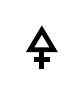
\begin{tikzpicture}[baseline=0mm, line width=0.6mm, line cap=butt]
  \draw (0,-2mm) -- (0,0.5mm);
  \draw (-1mm,-0.75mm) -- (1mm,-0.75mm);
  \draw (-1.5mm,0.5mm) -- (0,3mm) -- (1.5mm,0.5mm) -- cycle;
\end{tikzpicture}}}
% Salt: circle with horizontal line through middle (matches \alcsalt)
\newcommand{\tinysalt}{\raisebox{-1mm}{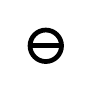
\begin{tikzpicture}[baseline=0mm, line width=0.6mm]
  \draw (0,0) circle (2mm);
  \draw (-2mm,0) -- (2mm,0);
\end{tikzpicture}}}
% Mercury: cross below, U-arc on top (matches \alcmercury)
\newcommand{\tinymercury}{\raisebox{-2mm}{
\begin{tikzpicture}[baseline=0mm, line width=0.6mm, line cap=butt]
  \draw (0,-2.75mm) -- (0,-0.5mm);
  \draw (-1mm,-1.5mm) -- (1mm,-1.5mm);
  \draw (-1mm,1.8mm) -- (-1mm,0.5mm) arc (180:360:1mm) -- (1mm,1.8mm);
\end{tikzpicture}}}
% Elemental triangles
\newcommand{\tinyfire}{\raisebox{-0.5mm}{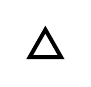
\begin{tikzpicture}[baseline=0mm, line width=0.5mm]
  \draw (-2mm,0) -- (0,3.5mm) -- (2mm,0) -- cycle;
\end{tikzpicture}}}
\newcommand{\tinywater}{\raisebox{-0.5mm}{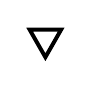
\begin{tikzpicture}[baseline=0mm, line width=0.5mm]
  \draw (-2mm,3.5mm) -- (0,0) -- (2mm,3.5mm) -- cycle;
\end{tikzpicture}}}
\newcommand{\tinyair}{\raisebox{-0.5mm}{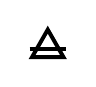
\begin{tikzpicture}[baseline=0mm, line width=0.5mm]
  \draw (-2mm,0) -- (0,3.5mm) -- (2mm,0) -- cycle;
  \draw (-2.3mm,1.1mm) -- (2.3mm,1.1mm);
\end{tikzpicture}}}
\newcommand{\tinyearth}{\raisebox{-0.5mm}{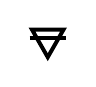
\begin{tikzpicture}[baseline=0mm, line width=0.5mm]
  \draw (-2mm,3.5mm) -- (0,0) -- (2mm,3.5mm) -- cycle;
  \draw (-2.3mm,2.4mm) -- (2.3mm,2.4mm);
\end{tikzpicture}}}

% Alchemical Sulfur: upward triangle above a cross
\newcommand{\alcsulfur}{%
  % Li trigram (Fire) — left side: solid (red top), broken, solid
  \begin{scope}[shift={(0.5\cardwidth-23mm,0.52\cardheight)}, line width=2mm, line cap=butt]
    % Top line — solid, red
    \draw[red] (-4mm,5mm) -- (4mm,5mm);
    % Middle line — broken
    \draw (-4mm,0mm) -- (-1mm,0mm);
    \draw (1mm,0mm) -- (4mm,0mm);
    % Bottom line — solid
    \draw (-4mm,-5mm) -- (4mm,-5mm);
    % Labels
    \node[above, font=\cardfont\fontsize{14}{16}\selectfont] at (0,6mm) {Lí};
    \node[below, font=\cardfont\fontsize{10}{12}\selectfont] at (0,-6mm) {Fire};
  \end{scope}%
  % Qian trigram (Heaven) — right side: all solid (yellow top)
  \begin{scope}[shift={(0.5\cardwidth+23mm,0.52\cardheight)}, line width=2mm, line cap=butt]
    % Top line — solid, yellow
    \draw[yellow!70!orange] (-4mm,5mm) -- (4mm,5mm);
    % Middle line — solid
    \draw (-4mm,0mm) -- (4mm,0mm);
    % Bottom line — solid
    \draw (-4mm,-5mm) -- (4mm,-5mm);
    % Labels
    \node[above, font=\cardfont\fontsize{14}{16}\selectfont] at (0,6mm) {Qián};
    \node[below, font=\cardfont\fontsize{10}{12}\selectfont] at (0,-6mm) {Heaven};
  \end{scope}%
  \begin{scope}[shift={(0.5\cardwidth,0.52\cardheight)}, magenta, line width=3.5mm]
    % Cross — vertical bar from bottom up to where triangle begins
    \draw (0,-24mm) -- (0,3mm);
    \draw (-12mm,-12mm) -- (12mm,-12mm); % horizontal bar
    % Upward-pointing triangle
    \draw (-14mm,3mm) -- (0,28mm) -- (14mm,3mm) -- cycle;
  \end{scope}%
  % 〇并 below Shin (vertical)
  \node[anchor=north east, text=black, font=\cjkfallback\fontsize{14}{16}\selectfont,
    inner sep=1.5mm] at (\cardwidth, \cardheight-6mm) {〇};
  \node[anchor=north east, text=black, font=\cjkfontgb\fontsize{14}{16}\selectfont,
    inner sep=1.5mm] at (\cardwidth, \cardheight-11mm) {并};
  % Sulfur
  \node[anchor=north, text=black, font=\cardfont\fontsize{17}{19}\selectfont]
    at (0.5\cardwidth, 0.52\cardheight-24mm) {Sulfur};
  % c a r d i n a l
  \node[anchor=north, text=black, font=\cardfont\fontsize{9}{11}\selectfont]
    at (0.5\cardwidth, 0.52\cardheight-31mm) {c\enspace a\enspace r\enspace d\enspace i\enspace n\enspace a\enspace l};
  % Spirit
  \node[anchor=north, text=black, font=\cardfont\fontsize{17}{19}\selectfont]
    at (0.5\cardwidth, 0.52\cardheight-34mm) {Spirit};
  % נשמה above neshama
  \node[anchor=base, text=black, font=\hebrewfont\fontsize{14}{16}\selectfont]
    at (0.5\cardwidth-21mm, 0.52\cardheight-40.5mm) {נשמה};
  \node[anchor=base, text=black, font=\cardfont\fontsize{10}{12}\selectfont]
    at (0.5\cardwidth-21mm, 0.52\cardheight-43mm) {neshama};
  % pitta with पित्त below
  \node[anchor=base, text=black, font=\cardfont\fontsize{10}{12}\selectfont]
    at (0.5\cardwidth, 0.52\cardheight-43mm) {pitta};
  \node[anchor=north, text=black, font=\devfont\fontsize{14}{16}\selectfont]
    at (0.5\cardwidth, 0.52\cardheight-42.5mm) {पित्त};
  % 神 above shén
  \node[anchor=base, text=black, font=\cjkfont\fontsize{18}{20}\selectfont]
    at (0.5\cardwidth+21mm, 0.52\cardheight-40.5mm) {神};
  \node[anchor=base, text=black, font=\cardfont\fontsize{10}{12}\selectfont]
    at (0.5\cardwidth+21mm, 0.52\cardheight-43mm) {shén};
  % fire & water
  \node[anchor=base east, text=black, font=\cardfont\fontsize{10}{12}\selectfont]
    at (0.5\cardwidth-1mm, 0.52\cardheight-52mm) {fire};
  \node[anchor=base, text=black, font=\cardfont\fontsize{10}{12}\selectfont]
    at (0.5\cardwidth, 0.52\cardheight-52mm) {\&};
  \node[anchor=base west, text=black, font=\cardfont\fontsize{10}{12}\selectfont]
    at (0.5\cardwidth+1mm, 0.52\cardheight-52mm) {water};
  % Lot of Spirit — circle pierced by vertical line (phi-like), bottom left
  \begin{scope}[shift={(7mm,4mm)}]
    \draw[thick] (0,0) circle (2.5mm);
    \draw[thick] (0,-3.2mm) -- (0,3.2mm);
    % "Lot of Spirit" curved above
    \path[postaction={decorate, decoration={text along path,
      text={|\cardfont\fontsize{5}{6}\selectfont|Lot of Spirit},
      text align=center, raise=0pt}}]
      (190:3.5mm) arc (190:-10:3.5mm);
  \end{scope}%
  % Red dragon 中 — bottom right
  \begin{scope}[shift={(\cardwidth-7mm,5mm)}]
    \node[anchor=center, text=red, font=\cjkfont\fontsize{18}{20}\selectfont]
      at (0,0) {中};
    % "hóng zhōng" curved above
    \path[postaction={decorate, decoration={text along path,
      text={|\cardfont\fontsize{5}{6}\selectfont\color{red}|hóng zhōng},
      text align=center, raise=0pt}}]
      (170:3mm) arc (170:10:3mm);
    % "bullseye" curved below
    \path[postaction={decorate, decoration={text along path,
      text={|\cardfont\fontsize{5}{6}\selectfont\color{red}|bullseye},
      text align=center, raise=1pt, reverse path}}]
      (-10:4.5mm) arc (-10:-170:4.5mm);
  \end{scope}%
}

% Alchemical Salt: circle with horizontal line through middle
\newcommand{\alcsalt}{%
  \begin{scope}[shift={(0.5\cardwidth,0.52\cardheight)}, cyan, line width=3.5mm]
    \draw (0,0) circle (14mm);
    \draw (-14mm,0) -- (14mm,0);
  \end{scope}%
  % Kan trigram (Water) — left side: broken, solid, broken (bottom line blue)
  \begin{scope}[shift={(0.5\cardwidth-23mm,0.52\cardheight)}, line width=2mm, line cap=butt]
    % Top line — broken
    \draw (-4mm,5mm) -- (-1mm,5mm);
    \draw (1mm,5mm) -- (4mm,5mm);
    % Middle line — solid
    \draw (-4mm,0mm) -- (4mm,0mm);
    % Bottom line — broken, blue
    \draw[blue] (-4mm,-5mm) -- (-1mm,-5mm);
    \draw[blue] (1mm,-5mm) -- (4mm,-5mm);
    % Labels
    \node[above, font=\cardfont\fontsize{14}{16}\selectfont] at (0,6mm) {Kǎn};
    \node[below, font=\cardfont\fontsize{10}{12}\selectfont] at (0,-6mm) {Water};
  \end{scope}%
  % Kun trigram (Earth) — right side: all broken (bottom line green)
  \begin{scope}[shift={(0.5\cardwidth+23mm,0.52\cardheight)}, line width=2mm, line cap=butt]
    % Top line — broken
    \draw (-4mm,5mm) -- (-1mm,5mm);
    \draw (1mm,5mm) -- (4mm,5mm);
    % Middle line — broken
    \draw (-4mm,0mm) -- (-1mm,0mm);
    \draw (1mm,0mm) -- (4mm,0mm);
    % Bottom line — broken, green
    \draw[green!50!black] (-4mm,-5mm) -- (-1mm,-5mm);
    \draw[green!50!black] (1mm,-5mm) -- (4mm,-5mm);
    % Labels
    \node[above, font=\cardfont\fontsize{14}{16}\selectfont] at (0,6mm) {Kūn};
    \node[below, font=\cardfont\fontsize{10}{12}\selectfont] at (0,-6mm) {Earth};
  \end{scope}%
  % 半并 below Mem (vertical)
  \node[anchor=north east, text=black, font=\cjkfontgb\fontsize{14}{16}\selectfont,
    inner sep=1.5mm] at (\cardwidth, \cardheight-6mm) {半};
  \node[anchor=north east, text=black, font=\cjkfontgb\fontsize{14}{16}\selectfont,
    inner sep=1.5mm] at (\cardwidth, \cardheight-11mm) {并};
  % Salt
  \node[anchor=north, text=black, font=\cardfont\fontsize{17}{19}\selectfont]
    at (0.5\cardwidth, 0.52\cardheight-24mm) {Salt};
  % f i x e d
  \node[anchor=north, text=black, font=\cardfont\fontsize{9}{11}\selectfont]
    at (0.5\cardwidth, 0.52\cardheight-31mm) {f\enspace i\enspace x\enspace e\enspace d};
  % Essence
  \node[anchor=north, text=black, font=\cardfont\fontsize{17}{19}\selectfont]
    at (0.5\cardwidth, 0.52\cardheight-34mm) {Essence};
  % נפש above nefesh
  \node[anchor=base, text=black, font=\hebrewfont\fontsize{14}{16}\selectfont]
    at (0.5\cardwidth-21mm, 0.52\cardheight-40.5mm) {נפש};
  \node[anchor=base, text=black, font=\cardfont\fontsize{10}{12}\selectfont]
    at (0.5\cardwidth-21mm, 0.52\cardheight-43mm) {nefesh};
  % kapha
  \node[anchor=base, text=black, font=\cardfont\fontsize{10}{12}\selectfont]
    at (0.5\cardwidth, 0.52\cardheight-43mm) {kapha};
  % कफ below kapha
  \node[anchor=north, text=black, font=\devfont\fontsize{14}{16}\selectfont]
    at (0.5\cardwidth, 0.52\cardheight-42.5mm) {कफ};
  % 精 above jīng
  \node[anchor=base, text=black, font=\cjkfont\fontsize{18}{20}\selectfont]
    at (0.5\cardwidth+21mm, 0.52\cardheight-40.5mm) {精};
  \node[anchor=base, text=black, font=\cardfont\fontsize{10}{12}\selectfont]
    at (0.5\cardwidth+21mm, 0.52\cardheight-43mm) {jīng};
  % Lot of Fortune — circle with X inside, bottom left
  \begin{scope}[shift={(7mm,4mm)}]
    \draw[thick] (0,0) circle (2.5mm);
    \draw[thick] (-1.7mm,1.7mm) -- (1.7mm,-1.7mm);
    \draw[thick] (-1.7mm,-1.7mm) -- (1.7mm,1.7mm);
    % "Lot of Fortune" curved above
    \path[postaction={decorate, decoration={text along path,
      text={|\cardfont\fontsize{5}{6}\selectfont|Lot of Fortune},
      text align=center, raise=0pt}}]
      (190:3.5mm) arc (190:-10:3.5mm);
  \end{scope}%
  % Blank mahjong tile — bottom right
  \begin{scope}[shift={(\cardwidth-7mm,5mm)}]
    \draw[thick, rounded corners=0.3mm] (-2mm,-2.5mm) rectangle (2mm,2.5mm);
    \draw[thin, rounded corners=0.2mm] (-1.4mm,-1.8mm) rectangle (1.4mm,1.8mm);
    % Corner diagonals inside inner frame
    \draw[thin] (-1.4mm,1.4mm) -- (-0.8mm,1.8mm);
    \draw[thin] (1.4mm,1.4mm) -- (0.8mm,1.8mm);
    \draw[thin] (-1.4mm,-1.4mm) -- (-0.8mm,-1.8mm);
    \draw[thin] (1.4mm,-1.4mm) -- (0.8mm,-1.8mm);
    % "bái bǎu" curved above
    \path[postaction={decorate, decoration={text along path,
      text={|\cardfont\fontsize{5}{6}\selectfont|bái bǎu},
      text align=center, raise=0pt}}]
      (170:3.5mm) arc (170:10:3.5mm);
    % "clean slate" curved below
    \path[postaction={decorate, decoration={text along path,
      text={|\cardfont\fontsize{5}{6}\selectfont|clean slate},
      text align=center, raise=1pt, reverse path}}]
      (-10:4.5mm) arc (-10:-170:4.5mm);
  \end{scope}%
  % water & earth
  \node[anchor=base east, text=black, font=\cardfont\fontsize{10}{12}\selectfont]
    at (0.5\cardwidth-1mm, 0.52\cardheight-52mm) {water};
  \node[anchor=base, text=black, font=\cardfont\fontsize{10}{12}\selectfont]
    at (0.5\cardwidth, 0.52\cardheight-52mm) {\&};
  \node[anchor=base west, text=black, font=\cardfont\fontsize{10}{12}\selectfont]
    at (0.5\cardwidth+1mm, 0.52\cardheight-52mm) {earth};
}

% Alchemical Mercury variant: U (crescent) directly above a cross, no circle
\newcommand{\alcmercury}{%
  \begin{scope}[shift={(0.5\cardwidth,0.52\cardheight)}, yellow!80!orange, line width=3.5mm]
    % Cross — vertical bar from bottom up to where U begins
    \draw (0,-24mm) -- (0,0mm);
    \draw (-12mm,-12mm) -- (12mm,-12mm); % horizontal bar
    % U (open arc) sitting on top of the cross
    \draw (-14mm,28mm) -- (-14mm,14mm) arc (180:360:14mm) -- (14mm,28mm);
  \end{scope}%
  % 万千 below Aleph (vertical)
  \node[anchor=north east, text=black, font=\cjkfontgb\fontsize{14}{16}\selectfont,
    inner sep=1.5mm] at (\cardwidth, \cardheight-6mm) {千};
  \node[anchor=north east, text=black, font=\cjkfontgb\fontsize{14}{16}\selectfont,
    inner sep=1.5mm] at (\cardwidth, \cardheight-11mm) {万};
  % QUICKSILVER label below Mercury symbol
  \node[anchor=north, text=black, font=\cardfont\fontsize{17}{19}\selectfont]
    at (0.5\cardwidth, 0.52\cardheight-24mm) {Quicksilver};
  \node[anchor=north, text=black, font=\cardfont\fontsize{9}{11}\selectfont]
    at (0.5\cardwidth, 0.52\cardheight-31mm) {m\enspace u\enspace t\enspace a\enspace b\enspace l\enspace e};
  \node[anchor=north, text=black, font=\cardfont\fontsize{17}{19}\selectfont]
    at (0.5\cardwidth, 0.52\cardheight-34mm) {Breath};
  \node[anchor=base, text=black, font=\hebrewfont\fontsize{14}{16}\selectfont]
    at (0.5\cardwidth-21mm, 0.52\cardheight-40.5mm) {רוח};
  \node[anchor=base, text=black, font=\cardfont\fontsize{10}{12}\selectfont]
    at (0.5\cardwidth-21mm, 0.52\cardheight-43mm) {ruach};
  \node[anchor=base, text=black, font=\cardfont\fontsize{10}{12}\selectfont]
    at (0.5\cardwidth, 0.52\cardheight-43mm) {vāta};
  \node[anchor=north, text=black, font=\devfont\fontsize{14}{16}\selectfont]
    at (0.5\cardwidth, 0.52\cardheight-42.5mm) {वात};
  \node[anchor=base east, text=black, font=\cardfont\fontsize{10}{12}\selectfont]
    at (0.5\cardwidth-1mm, 0.52\cardheight-52mm) {air};
  \node[anchor=base, text=black, font=\cardfont\fontsize{10}{12}\selectfont]
    at (0.5\cardwidth, 0.52\cardheight-52mm) {\&};
  \node[anchor=base west, text=black, font=\cardfont\fontsize{10}{12}\selectfont]
    at (0.5\cardwidth+1mm, 0.52\cardheight-52mm) {void};
  \node[anchor=base, text=black, font=\cjkfont\fontsize{18}{20}\selectfont]
    at (0.5\cardwidth+21mm, 0.52\cardheight-40.5mm) {氣};
  \node[anchor=base, text=black, font=\cardfont\fontsize{10}{12}\selectfont]
    at (0.5\cardwidth+21mm, 0.52\cardheight-43mm) {qi};
  % Kan trigram (Water) — left side: broken, solid (blue), broken
  \begin{scope}[shift={(0.5\cardwidth-23mm,0.52\cardheight)}, line width=2mm, line cap=butt]
    % Top line — broken
    \draw (-4mm,5mm) -- (-1mm,5mm);
    \draw (1mm,5mm) -- (4mm,5mm);
    % Middle line — solid, blue
    \draw[blue] (-4mm,0mm) -- (4mm,0mm);
    % Bottom line — broken
    \draw (-4mm,-5mm) -- (-1mm,-5mm);
    \draw (1mm,-5mm) -- (4mm,-5mm);
    % Labels
    \node[above, font=\cardfont\fontsize{14}{16}\selectfont] at (0,6mm) {Kǎn};
    \node[below, font=\cardfont\fontsize{10}{12}\selectfont] at (0,-6mm) {Water};
  \end{scope}%
  % Li trigram (Fire) — right side: solid, broken (red), solid
  \begin{scope}[shift={(0.5\cardwidth+23mm,0.52\cardheight)}, line width=2mm, line cap=butt]
    % Top line — solid
    \draw (-4mm,5mm) -- (4mm,5mm);
    % Middle line — broken, red
    \draw[red] (-4mm,0mm) -- (-1mm,0mm);
    \draw[red] (1mm,0mm) -- (4mm,0mm);
    % Bottom line — solid
    \draw (-4mm,-5mm) -- (4mm,-5mm);
    % Labels
    \node[above, font=\cardfont\fontsize{14}{16}\selectfont] at (0,6mm) {Lí};
    \node[below, font=\cardfont\fontsize{10}{12}\selectfont] at (0,-6mm) {Fire};
  \end{scope}%
  % Lot of Eros — heart in circle with curved text, bottom left
  \begin{scope}[shift={(7mm,4mm)}]
    \draw[thick] (0,0) circle (2.5mm);
    % Heart
    \draw[thick] (0,0.7mm)
      .. controls (-0.8mm,2.1mm) and (-2mm,1.3mm) .. (-2mm,0.5mm)
      .. controls (-2mm,-0.3mm) and (0,-1.5mm) .. (0,-1.8mm)
      .. controls (0,-1.5mm) and (2mm,-0.3mm) .. (2mm,0.5mm)
      .. controls (2mm,1.3mm) and (0.8mm,2.1mm) .. (0,0.7mm);
    % "Lot of" curved above
    \path[postaction={decorate, decoration={text along path,
      text={|\cardfont\fontsize{5}{6}\selectfont|Lot of Eros},
      text align=center, raise=0pt}}]
      (170:3.5mm) arc (170:10:3.5mm);
  \end{scope}%
  % 發 (hatsu/green dragon) — bottom right
  \begin{scope}[shift={(\cardwidth-7mm,5mm)}]
    \node[anchor=center, text=green!50!black, font=\cjkfont\fontsize{18}{20}\selectfont]
      at (0,0) {發};
    % "fa cái" curved above
    \path[postaction={decorate, decoration={text along path,
      text={|\cardfont\fontsize{5}{6}\selectfont\color{green!50!black}|fā cái},
      text align=center, raise=0pt}}]
      (170:3mm) arc (170:10:3mm);
    % "strike it rich" curved below
    \path[postaction={decorate, decoration={text along path,
      text={|\cardfont\fontsize{5}{6}\selectfont\color{green!50!black}|strike  it  rich},
      text align=center, raise=1pt, reverse path}}]
      (-10:4.5mm) arc (-10:-170:4.5mm);
  \end{scope}%
  \jokertext{black}
}

% Vertical JOKER on both sides, parameterized by color
\newcommand{\jokertext}[1]{%
  \foreach \letter/\i in {J/0,O/1,K/2,E/3,R/4} {
    \node[anchor=center, text=#1, font=\rankfont\fontsize{12}{14}\selectfont]
      at (2.5mm, \cardheight-11mm-\i*5mm) {\letter};
  }
  \foreach \letter/\i in {J/0,O/1,K/2,E/3,R/4} {
    \node[anchor=center, rotate=180, text=#1, font=\rankfont\fontsize{12}{14}\selectfont]
      at (\cardwidth-2.5mm, 11mm+\i*5mm) {\letter};
  }
}

% Traditional Mercury symbol (Unicode glyph, orange)
\newcommand{\alcmercurytrad}{%
  \node[anchor=center, text=orange, font=\symbserif\fontsize{160}{170}\selectfont]
    at (0.5\cardwidth, 0.52\cardheight) {☿};
  % Kǎn trigram (Water) — left side: broken, solid, broken
  \begin{scope}[shift={(0.5\cardwidth-23mm,0.52\cardheight)}, line width=2mm, line cap=butt]
    \draw (-4mm,5mm) -- (-1mm,5mm); \draw (1mm,5mm) -- (4mm,5mm);
    \draw (-4mm,0mm) -- (4mm,0mm);
    \draw (-4mm,-5mm) -- (-1mm,-5mm); \draw (1mm,-5mm) -- (4mm,-5mm);
    \node[above, font=\cardfont\fontsize{14}{16}\selectfont] at (0,6mm) {Kǎn};
    \node[below, font=\cardfont\fontsize{10}{12}\selectfont] at (0,-6mm) {Water};
  \end{scope}%
  % Kǎn trigram (Water) — right side
  \begin{scope}[shift={(0.5\cardwidth+23mm,0.52\cardheight)}, line width=2mm, line cap=butt]
    \draw (-4mm,5mm) -- (-1mm,5mm); \draw (1mm,5mm) -- (4mm,5mm);
    \draw (-4mm,0mm) -- (4mm,0mm);
    \draw (-4mm,-5mm) -- (-1mm,-5mm); \draw (1mm,-5mm) -- (4mm,-5mm);
    \node[above, font=\cardfont\fontsize{14}{16}\selectfont] at (0,6mm) {Kǎn};
    \node[below, font=\cardfont\fontsize{10}{12}\selectfont] at (0,-6mm) {Water};
  \end{scope}%
  % Mercury
  \node[anchor=north, text=black, font=\cardfont\fontsize{17}{19}\selectfont]
    at (0.5\cardwidth, 0.52\cardheight-24mm) {Mercury};
  \node[anchor=north, text=black, font=\cardfont\fontsize{9}{11}\selectfont]
    at (0.5\cardwidth, \cardheight-6mm) {Benefic/Malefic of Day \& Night};
  \node[anchor=base east, text=black, font=\cardfont\fontsize{9}{11}\selectfont, inner xsep=3mm]
    at (0.5\cardwidth, \cardheight-13mm) {\resizebox{12mm}{\height}{exalted in}};
  \node[anchor=base, text=black, font=\symbserif\fontsize{12}{14}\selectfont]
    at (0.5\cardwidth, \cardheight-13mm) {♍};
  \node[anchor=base west, text=black, font=\cardfont\fontsize{9}{11}\selectfont, inner xsep=3mm]
    at (0.5\cardwidth, \cardheight-13mm) {Virgo};
  \node[anchor=north, text=black, font=\cardfont\fontsize{9}{11}\selectfont]
    at (0.5\cardwidth, 0.52\cardheight-30mm) {Joy in 1\textsuperscript{st} House of Self};
  \node[anchor=north, text=black, font=\cardfont\fontsize{17}{19}\selectfont]
    at (0.5\cardwidth, 0.52\cardheight-34mm) {Brilliance};
  % Wuxing Water
  \node[anchor=base, text=black, font=\cardfont\fontsize{10}{12}\selectfont]
    at (0.5\cardwidth, 0.52\cardheight-43mm) {shuǐ};
  \foreach \dx/\dy in {0.3/0,-0.3/0,0/0.3,0/-0.3,0.2/0.2,-0.2/0.2,0.2/-0.2,-0.2/-0.2} {
    \node[anchor=north, text=black!50, opacity=0.5, font=\cjkfont\fontsize{18}{20}\selectfont]
      at ([xshift=\dx mm, yshift=\dy mm]0.5\cardwidth, 0.52\cardheight-42.5mm) {水};
  }
  \node[anchor=north, text=black, font=\cjkfont\fontsize{18}{20}\selectfont]
    at (0.5\cardwidth, 0.52\cardheight-42.5mm) {水};
  \node[anchor=north, text=black, font=\cardfont\fontsize{10}{12}\selectfont]
    at (0.5\cardwidth, 0.52\cardheight-49mm) {water};
  % Heavenly stems — Water: 壬 rén (9 Yang), 癸 guǐ (10 Yin)
  \node[anchor=base, text=black, font=\cardfont\fontsize{7}{8}\selectfont]
    at (0.5\cardwidth-9mm, 0.52\cardheight-43mm) {rén};
  \node[anchor=north, text=black, font=\cjkfont\fontsize{10}{11}\selectfont]
    at (0.5\cardwidth-9mm, 0.52\cardheight-42.5mm) {壬};
  \node[anchor=north, text=black, font=\cardfont\fontsize{7}{8}\selectfont]
    at (0.5\cardwidth-9mm, 0.52\cardheight-46mm) {9};
  \node[anchor=base, text=black, font=\cardfont\fontsize{7}{8}\selectfont]
    at (0.5\cardwidth+9mm, 0.52\cardheight-43mm) {guǐ};
  \node[anchor=north, text=black, font=\cjkfont\fontsize{10}{11}\selectfont]
    at (0.5\cardwidth+9mm, 0.52\cardheight-42.5mm) {癸};
  \node[anchor=north, text=black, font=\cardfont\fontsize{7}{8}\selectfont]
    at (0.5\cardwidth+9mm, 0.52\cardheight-46mm) {10};
  \node[anchor=center, text=black, font=\greekfont\fontsize{18}{20}\selectfont]
    at (7mm, 5mm) {Ε};
  \begin{scope}[shift={(\cardwidth-11mm,5mm)}]
    \node[anchor=center, inner sep=0pt] at (0,0) {\includegraphics[width=14mm]{images/chakra6}};
    \path[postaction={decorate, decoration={text along path,
      text={|\cardfont\fontsize{7}{8}\selectfont\color{blue!50!violet}|Third Eye},
      text align=center, raise=0pt}}]
      (170:6mm) arc (170:10:6mm);
  \end{scope}%
  \jokertext{red}
}

% Venus (Empress) — green
\newcommand{\plvenus}{%
  \node[anchor=center, text=green!50!black, font=\symbserif\fontsize{160}{170}\selectfont]
    at (0.5\cardwidth, 0.52\cardheight) {♀};
  % Qián trigram (Heaven) — left side: all solid
  \begin{scope}[shift={(0.5\cardwidth-23mm,0.52\cardheight)}, line width=2mm, line cap=butt]
    \draw (-4mm,5mm) -- (4mm,5mm);
    \draw (-4mm,0mm) -- (4mm,0mm);
    \draw (-4mm,-5mm) -- (4mm,-5mm);
    \node[above, font=\cardfont\fontsize{14}{16}\selectfont] at (0,6mm) {Qián};
    \node[below, font=\cardfont\fontsize{10}{12}\selectfont] at (0,-6mm) {Heaven};
  \end{scope}%
  % Duì trigram (Lake) — right side: broken top, solid, solid
  \begin{scope}[shift={(0.5\cardwidth+23mm,0.52\cardheight)}, line width=2mm, line cap=butt]
    \draw (-4mm,5mm) -- (-1mm,5mm); \draw (1mm,5mm) -- (4mm,5mm);
    \draw (-4mm,0mm) -- (4mm,0mm);
    \draw (-4mm,-5mm) -- (4mm,-5mm);
    \node[above, font=\cardfont\fontsize{14}{16}\selectfont] at (0,6mm) {Duì};
    \node[below, font=\cardfont\fontsize{10}{12}\selectfont] at (0,-6mm) {Lake};
  \end{scope}%
  \node[anchor=north, text=black, font=\cardfont\fontsize{17}{19}\selectfont]
    at (0.5\cardwidth, 0.52\cardheight-24mm) {Venus};
  \node[anchor=north, text=black, font=\cardfont\fontsize{9}{11}\selectfont]
    at (0.5\cardwidth, \cardheight-6mm) {Benefic of Night};
  \node[anchor=base east, text=black, font=\cardfont\fontsize{9}{11}\selectfont, inner xsep=3mm]
    at (0.5\cardwidth, \cardheight-13mm) {\resizebox{12mm}{\height}{exalted in}};
  \node[anchor=base, text=black, font=\symbserif\fontsize{12}{14}\selectfont]
    at (0.5\cardwidth, \cardheight-13mm) {♓};
  \node[anchor=base west, text=black, font=\cardfont\fontsize{9}{11}\selectfont, inner xsep=3mm]
    at (0.5\cardwidth, \cardheight-13mm) {Pisces};
  \node[anchor=north, text=black, font=\cardfont\fontsize{9}{11}\selectfont]
    at (0.5\cardwidth, 0.52\cardheight-30mm) {Joy in 5\textsuperscript{th} H. of Good Fortune};
  \node[anchor=north, text=black, font=\cardfont\fontsize{17}{19}\selectfont]
    at (0.5\cardwidth, 0.52\cardheight-34mm) {Beauty};
  % Wuxing Metal
  \node[anchor=base, text=black, font=\cardfont\fontsize{10}{12}\selectfont]
    at (0.5\cardwidth, 0.52\cardheight-43mm) {jīn};
  \foreach \dx/\dy in {0.6/0,-0.6/0,0/0.6,0/-0.6,0.4/0.4,-0.4/0.4,0.4/-0.4,-0.4/-0.4,0.3/0,-0.3/0,0/0.3,0/-0.3,0.2/0.2,-0.2/0.2,0.2/-0.2,-0.2/-0.2} {
    \node[anchor=north, text=white, opacity=0.4, font=\cjkfont\fontsize{18}{20}\selectfont]
      at ([xshift=\dx mm, yshift=\dy mm]0.5\cardwidth, 0.52\cardheight-42.5mm) {金};
  }
  \node[anchor=north, text=black, font=\cjkfont\fontsize{18}{20}\selectfont]
    at (0.5\cardwidth, 0.52\cardheight-42.5mm) {金};
  \node[anchor=north, text=black, font=\cardfont\fontsize{10}{12}\selectfont]
    at (0.5\cardwidth, 0.52\cardheight-49mm) {metal};
  % Heavenly stems — Metal: 庚 gēng (7 Yang), 辛 xīn (8 Yin)
  \node[anchor=base, text=black, font=\cardfont\fontsize{7}{8}\selectfont]
    at (0.5\cardwidth-9mm, 0.52\cardheight-43mm) {gēng};
  \node[anchor=north, text=black, font=\cjkfont\fontsize{10}{11}\selectfont]
    at (0.5\cardwidth-9mm, 0.52\cardheight-42.5mm) {庚};
  \node[anchor=north, text=black, font=\cardfont\fontsize{7}{8}\selectfont]
    at (0.5\cardwidth-9mm, 0.52\cardheight-46mm) {7};
  \node[anchor=base, text=black, font=\cardfont\fontsize{7}{8}\selectfont]
    at (0.5\cardwidth+9mm, 0.52\cardheight-43mm) {xīn};
  \node[anchor=north, text=black, font=\cjkfont\fontsize{10}{11}\selectfont]
    at (0.5\cardwidth+9mm, 0.52\cardheight-42.5mm) {辛};
  \node[anchor=north, text=black, font=\cardfont\fontsize{7}{8}\selectfont]
    at (0.5\cardwidth+9mm, 0.52\cardheight-46mm) {8};
  \node[anchor=center, text=black, font=\greekfont\fontsize{18}{20}\selectfont]
    at (7mm, 5mm) {Η};
  \begin{scope}[shift={(\cardwidth-9mm,7mm)}]
    \node[anchor=center, inner sep=0pt] at (0,0) {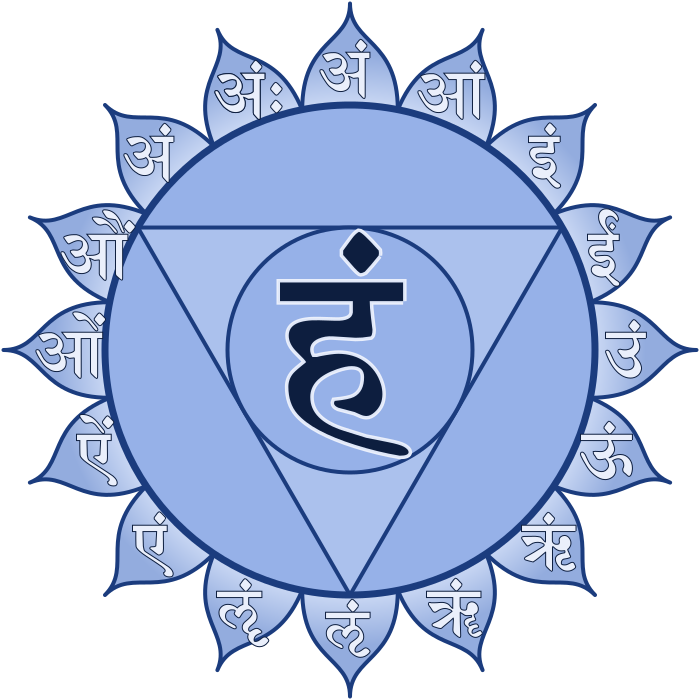
\includegraphics[width=14mm]{images/chakra5}};
    \path[postaction={decorate, decoration={text along path,
      text={|\cardfont\fontsize{7}{8}\selectfont\color{blue}|Voice},
      text align=center, raise=0pt}}]
      (170:8mm) arc (170:10:8mm);
  \end{scope}%
}

% Sun — yellow
\newcommand{\plsun}{%
  \node[anchor=center, text=yellow!80!orange, font=\symbfont\fontsize{160}{170}\selectfont]
    at (0.5\cardwidth, 0.52\cardheight) {☉};
  \node[anchor=north, text=black, font=\cardfont\fontsize{17}{19}\selectfont]
    at (0.5\cardwidth, 0.52\cardheight-24mm) {Sun};
  \node[anchor=north, text=black, font=\cardfont\fontsize{9}{11}\selectfont]
    at (0.5\cardwidth, \cardheight-6mm) {Luminary of Day};
  \node[anchor=base east, text=black, font=\cardfont\fontsize{9}{11}\selectfont, inner xsep=3mm]
    at (0.5\cardwidth, \cardheight-13mm) {\resizebox{12mm}{\height}{exalted in}};
  \node[anchor=base, text=black, font=\symbserif\fontsize{12}{14}\selectfont]
    at (0.5\cardwidth, \cardheight-13mm) {♈};
  \node[anchor=base west, text=black, font=\cardfont\fontsize{9}{11}\selectfont, inner xsep=3mm]
    at (0.5\cardwidth, \cardheight-13mm) {Aries};
  \node[anchor=north, text=black, font=\cardfont\fontsize{9}{11}\selectfont]
    at (0.5\cardwidth, 0.52\cardheight-30mm) {Joy in 9\textsuperscript{th} House of God};
  \node[anchor=north, text=black, font=\cardfont\fontsize{17}{19}\selectfont]
    at (0.5\cardwidth, 0.52\cardheight-34mm) {Glory};
  % 日 Sun / Yang
  \node[anchor=base, text=black, font=\cardfont\fontsize{10}{12}\selectfont]
    at (0.5\cardwidth, 0.52\cardheight-43mm) {rì};
  \node[anchor=north, text=black, font=\cjkfont\fontsize{18}{20}\selectfont]
    at (0.5\cardwidth, 0.52\cardheight-42.5mm) {日};
  \node[anchor=north, text=black, font=\cardfont\fontsize{10}{12}\selectfont]
    at (0.5\cardwidth, 0.52\cardheight-49mm) {yang};
  \node[anchor=center, text=black, font=\greekfont\fontsize{18}{20}\selectfont]
    at (7mm, 5mm) {Ι};
  \begin{scope}[shift={(\cardwidth-9mm,7mm)}]
    \node[anchor=center, inner sep=0pt] at (0,0) {\includegraphics[width=14mm]{images/chakra4}};
    \path[postaction={decorate, decoration={text along path,
      text={|\cardfont\fontsize{7}{8}\selectfont\color{green!50!black}|Heart},
      text align=center, raise=0pt}}]
      (170:8mm) arc (170:10:8mm);
  \end{scope}%
}

% Mars (Tower) — red
\newcommand{\plmars}{%
  \node[anchor=center, text=red, font=\symbserif\fontsize{160}{170}\selectfont]
    at (0.5\cardwidth, 0.52\cardheight) {♂};
  % Lí trigram (Fire) — left side: solid, broken, solid
  \begin{scope}[shift={(0.5\cardwidth-23mm,0.52\cardheight)}, line width=2mm, line cap=butt]
    \draw (-4mm,5mm) -- (4mm,5mm);
    \draw (-4mm,0mm) -- (-1mm,0mm); \draw (1mm,0mm) -- (4mm,0mm);
    \draw (-4mm,-5mm) -- (4mm,-5mm);
    \node[above, font=\cardfont\fontsize{14}{16}\selectfont] at (0,6mm) {Lí};
    \node[below, font=\cardfont\fontsize{10}{12}\selectfont] at (0,-6mm) {Fire};
  \end{scope}%
  % Lí trigram (Fire) — right side
  \begin{scope}[shift={(0.5\cardwidth+23mm,0.52\cardheight)}, line width=2mm, line cap=butt]
    \draw (-4mm,5mm) -- (4mm,5mm);
    \draw (-4mm,0mm) -- (-1mm,0mm); \draw (1mm,0mm) -- (4mm,0mm);
    \draw (-4mm,-5mm) -- (4mm,-5mm);
    \node[above, font=\cardfont\fontsize{14}{16}\selectfont] at (0,6mm) {Lí};
    \node[below, font=\cardfont\fontsize{10}{12}\selectfont] at (0,-6mm) {Fire};
  \end{scope}%
  \node[anchor=north, text=black, font=\cardfont\fontsize{17}{19}\selectfont]
    at (0.5\cardwidth, 0.52\cardheight-24mm) {Mars};
  \node[anchor=north, text=black, font=\cardfont\fontsize{9}{11}\selectfont]
    at (0.5\cardwidth, \cardheight-6mm) {Malefic of Night};
  \node[anchor=base east, text=black, font=\cardfont\fontsize{9}{11}\selectfont, inner xsep=3mm]
    at (0.5\cardwidth, \cardheight-13mm) {\resizebox{12mm}{\height}{exalted in}};
  \node[anchor=base, text=black, font=\symbserif\fontsize{12}{14}\selectfont]
    at (0.5\cardwidth, \cardheight-13mm) {♑};
  \node[anchor=base west, text=black, font=\cardfont\fontsize{9}{11}\selectfont, inner xsep=3mm]
    at (0.5\cardwidth, \cardheight-13mm) {Capricorn};
  \node[anchor=north, text=black, font=\cardfont\fontsize{9}{11}\selectfont]
    at (0.5\cardwidth, 0.52\cardheight-30mm) {Joy in 6\textsuperscript{th} H. of Bad Fortune};
  \node[anchor=north, text=black, font=\cardfont\fontsize{17}{19}\selectfont]
    at (0.5\cardwidth, 0.52\cardheight-34mm) {Power};
  % Wuxing Fire
  \node[anchor=base, text=black, font=\cardfont\fontsize{10}{12}\selectfont]
    at (0.5\cardwidth, 0.52\cardheight-43mm) {huǒ};
  \foreach \dx/\dy in {0.3/0,-0.3/0,0/0.3,0/-0.3,0.2/0.2,-0.2/0.2,0.2/-0.2,-0.2/-0.2} {
    \node[anchor=north, text=red, opacity=0.5, font=\cjkfont\fontsize{18}{20}\selectfont]
      at ([xshift=\dx mm, yshift=\dy mm]0.5\cardwidth, 0.52\cardheight-42.5mm) {火};
  }
  \node[anchor=north, text=black, font=\cjkfont\fontsize{18}{20}\selectfont]
    at (0.5\cardwidth, 0.52\cardheight-42.5mm) {火};
  \node[anchor=north, text=black, font=\cardfont\fontsize{10}{12}\selectfont]
    at (0.5\cardwidth, 0.52\cardheight-49mm) {fire};
  % Heavenly stems — Fire: 丙 bǐng (3 Yang), 丁 dīng (4 Yin)
  \node[anchor=base, text=black, font=\cardfont\fontsize{7}{8}\selectfont]
    at (0.5\cardwidth-9mm, 0.52\cardheight-43mm) {bǐng};
  \node[anchor=north, text=black, font=\cjkfont\fontsize{10}{11}\selectfont]
    at (0.5\cardwidth-9mm, 0.52\cardheight-42.5mm) {丙};
  \node[anchor=north, text=black, font=\cardfont\fontsize{7}{8}\selectfont]
    at (0.5\cardwidth-9mm, 0.52\cardheight-46mm) {3};
  \node[anchor=base, text=black, font=\cardfont\fontsize{7}{8}\selectfont]
    at (0.5\cardwidth+9mm, 0.52\cardheight-43mm) {dīng};
  \node[anchor=north, text=black, font=\cjkfont\fontsize{10}{11}\selectfont]
    at (0.5\cardwidth+9mm, 0.52\cardheight-42.5mm) {丁};
  \node[anchor=north, text=black, font=\cardfont\fontsize{7}{8}\selectfont]
    at (0.5\cardwidth+9mm, 0.52\cardheight-46mm) {4};
  \node[anchor=center, text=black, font=\greekfont\fontsize{18}{20}\selectfont]
    at (7mm, 5mm) {Ο};
  \begin{scope}[shift={(\cardwidth-9mm,7mm)}]
    \node[anchor=center, inner sep=0pt] at (0,0) {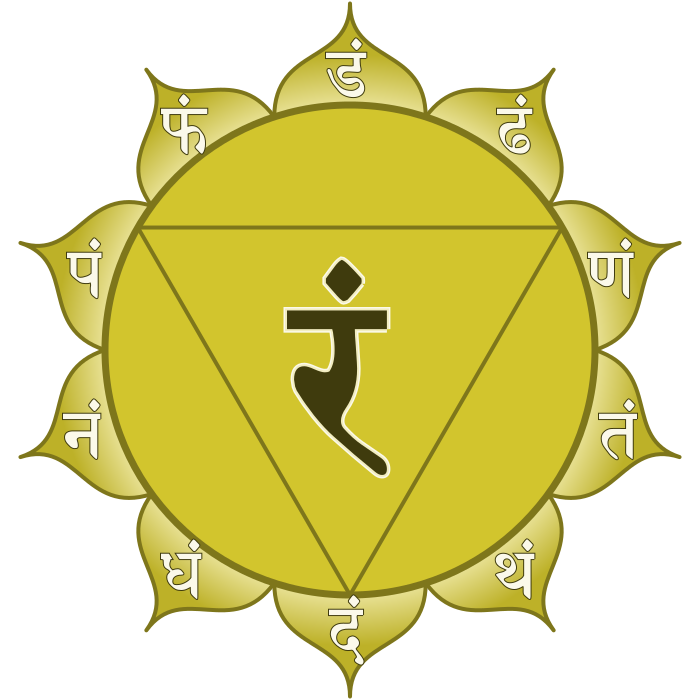
\includegraphics[width=14mm]{images/chakra3}};
    \path[postaction={decorate, decoration={text along path,
      text={|\cardfont\fontsize{7}{8}\selectfont\color{yellow!50!orange}|Solar Plexus},
      text align=center, raise=0pt}}]
      (170:8mm) arc (170:10:8mm);
  \end{scope}%
}

% Jupiter (Wheel of Fortune) — blue
\newcommand{\pljupiter}{%
  \node[anchor=center, text=blue, font=\symbserif\fontsize{160}{170}\selectfont]
    at (0.5\cardwidth, 0.52\cardheight) {♃};
  % Zhèn trigram (Thunder) — left side: broken, broken, solid
  \begin{scope}[shift={(0.5\cardwidth-23mm,0.52\cardheight)}, line width=2mm, line cap=butt]
    \draw (-4mm,5mm) -- (-1mm,5mm); \draw (1mm,5mm) -- (4mm,5mm);
    \draw (-4mm,0mm) -- (-1mm,0mm); \draw (1mm,0mm) -- (4mm,0mm);
    \draw (-4mm,-5mm) -- (4mm,-5mm);
    \node[above, font=\cardfont\fontsize{14}{16}\selectfont] at (0,6mm) {Zhèn};
    \node[below, font=\cardfont\fontsize{10}{12}\selectfont] at (0,-6mm) {\resizebox{12mm}{\height}{Thunder}};
  \end{scope}%
  % Xùn trigram (Wind) — right side: solid, solid, broken
  \begin{scope}[shift={(0.5\cardwidth+23mm,0.52\cardheight)}, line width=2mm, line cap=butt]
    \draw (-4mm,5mm) -- (4mm,5mm);
    \draw (-4mm,0mm) -- (4mm,0mm);
    \draw (-4mm,-5mm) -- (-1mm,-5mm); \draw (1mm,-5mm) -- (4mm,-5mm);
    \node[above, font=\cardfont\fontsize{14}{16}\selectfont] at (0,6mm) {Xùn};
    \node[below, font=\cardfont\fontsize{10}{12}\selectfont] at (0,-6mm) {Wind};
  \end{scope}%
  \node[anchor=north, text=black, font=\cardfont\fontsize{17}{19}\selectfont]
    at (0.5\cardwidth, 0.52\cardheight-24mm) {Jupiter};
  \node[anchor=north, text=black, font=\cardfont\fontsize{9}{11}\selectfont]
    at (0.5\cardwidth, \cardheight-6mm) {Benefic of Day};
  \node[anchor=base east, text=black, font=\cardfont\fontsize{9}{11}\selectfont, inner xsep=3mm]
    at (0.5\cardwidth, \cardheight-13mm) {\resizebox{12mm}{\height}{exalted in}};
  \node[anchor=base, text=black, font=\symbserif\fontsize{12}{14}\selectfont]
    at (0.5\cardwidth, \cardheight-13mm) {♋};
  \node[anchor=base west, text=black, font=\cardfont\fontsize{9}{11}\selectfont, inner xsep=3mm]
    at (0.5\cardwidth, \cardheight-13mm) {Cancer};
  \node[anchor=north, text=black, font=\cardfont\fontsize{9}{11}\selectfont]
    at (0.5\cardwidth, 0.52\cardheight-30mm) {Joy in 11\textsuperscript{th} H. of Good Spirit};
  \node[anchor=north, text=black, font=\cardfont\fontsize{17}{19}\selectfont]
    at (0.5\cardwidth, 0.52\cardheight-34mm) {Abundance};
  % Wuxing Wood
  \node[anchor=base, text=black, font=\cardfont\fontsize{10}{12}\selectfont]
    at (0.5\cardwidth, 0.52\cardheight-43mm) {mù};
  \foreach \dx/\dy in {0.3/0,-0.3/0,0/0.3,0/-0.3,0.2/0.2,-0.2/0.2,0.2/-0.2,-0.2/-0.2} {
    \node[anchor=north, text=green!50!black, opacity=0.5, font=\cjkfont\fontsize{18}{20}\selectfont]
      at ([xshift=\dx mm, yshift=\dy mm]0.5\cardwidth, 0.52\cardheight-42.5mm) {木};
  }
  \node[anchor=north, text=black, font=\cjkfont\fontsize{18}{20}\selectfont]
    at (0.5\cardwidth, 0.52\cardheight-42.5mm) {木};
  \node[anchor=north, text=black, font=\cardfont\fontsize{10}{12}\selectfont]
    at (0.5\cardwidth, 0.52\cardheight-49mm) {wood};
  % Heavenly stems — Wood: 甲 jiǎ (1 Yang), 乙 yǐ (2 Yin)
  \node[anchor=base, text=black, font=\cardfont\fontsize{7}{8}\selectfont]
    at (0.5\cardwidth-9mm, 0.52\cardheight-43mm) {jiǎ};
  \node[anchor=north, text=black, font=\cjkfont\fontsize{10}{11}\selectfont]
    at (0.5\cardwidth-9mm, 0.52\cardheight-42.5mm) {甲};
  \node[anchor=north, text=black, font=\cardfont\fontsize{7}{8}\selectfont]
    at (0.5\cardwidth-9mm, 0.52\cardheight-46mm) {1};
  \node[anchor=base, text=black, font=\cardfont\fontsize{7}{8}\selectfont]
    at (0.5\cardwidth+9mm, 0.52\cardheight-43mm) {yǐ};
  \node[anchor=north, text=black, font=\cjkfont\fontsize{10}{11}\selectfont]
    at (0.5\cardwidth+9mm, 0.52\cardheight-42.5mm) {乙};
  \node[anchor=north, text=black, font=\cardfont\fontsize{7}{8}\selectfont]
    at (0.5\cardwidth+9mm, 0.52\cardheight-46mm) {2};
  \node[anchor=center, text=black, font=\greekfont\fontsize{18}{20}\selectfont]
    at (7mm, 5mm) {Υ};
  \begin{scope}[shift={(\cardwidth-9mm,7mm)}]
    \node[anchor=center, inner sep=0pt] at (0,0) {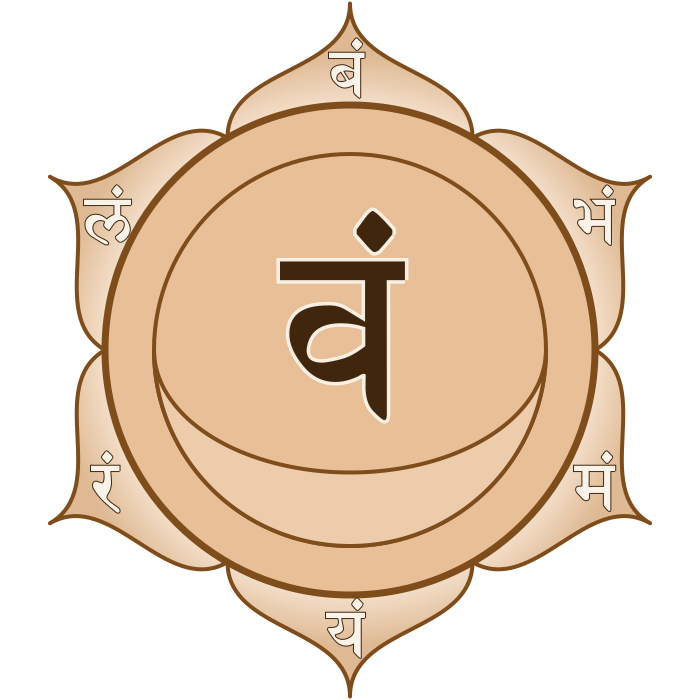
\includegraphics[width=14mm]{images/chakra2}};
    \path[postaction={decorate, decoration={text along path,
      text={|\cardfont\fontsize{7}{8}\selectfont\color{orange}|Sacral},
      text align=center, raise=0pt}}]
      (170:8mm) arc (170:10:8mm);
  \end{scope}%
}

% Saturn (World) — black
\newcommand{\plsaturn}{%
  \node[anchor=center, text=black, font=\symbserif\fontsize{160}{170}\selectfont]
    at (0.5\cardwidth, 0.52\cardheight) {♄};
  % Kūn trigram (Earth) — left side: all broken
  \begin{scope}[shift={(0.5\cardwidth-23mm,0.52\cardheight)}, line width=2mm, line cap=butt]
    \draw (-4mm,5mm) -- (-1mm,5mm); \draw (1mm,5mm) -- (4mm,5mm);
    \draw (-4mm,0mm) -- (-1mm,0mm); \draw (1mm,0mm) -- (4mm,0mm);
    \draw (-4mm,-5mm) -- (-1mm,-5mm); \draw (1mm,-5mm) -- (4mm,-5mm);
    \node[above, font=\cardfont\fontsize{14}{16}\selectfont] at (0,6mm) {Kūn};
    \node[below, font=\cardfont\fontsize{10}{12}\selectfont] at (0,-6mm) {Earth};
  \end{scope}%
  % Gèn trigram (Mountain) — right side: solid top, broken, broken
  \begin{scope}[shift={(0.5\cardwidth+23mm,0.52\cardheight)}, line width=2mm, line cap=butt]
    \draw (-4mm,5mm) -- (4mm,5mm);
    \draw (-4mm,0mm) -- (-1mm,0mm); \draw (1mm,0mm) -- (4mm,0mm);
    \draw (-4mm,-5mm) -- (-1mm,-5mm); \draw (1mm,-5mm) -- (4mm,-5mm);
    \node[above, font=\cardfont\fontsize{14}{16}\selectfont] at (0,6mm) {Gèn};
    \node[below, font=\cardfont\fontsize{10}{12}\selectfont] at (0,-6mm) {\resizebox{12mm}{\height}{Mountain}};
  \end{scope}%
  % Sect and Exaltation — under title
  \node[anchor=north, text=black, font=\cardfont\fontsize{9}{11}\selectfont]
    at (0.5\cardwidth, \cardheight-6mm) {Malefic of Day};
  \node[anchor=base east, text=black, font=\cardfont\fontsize{9}{11}\selectfont, inner xsep=3mm]
    at (0.5\cardwidth, \cardheight-13mm) {\resizebox{12mm}{\height}{exalted in}};
  \node[anchor=base, text=black, font=\symbserif\fontsize{12}{14}\selectfont]
    at (0.5\cardwidth, \cardheight-13mm) {♎};
  \node[anchor=base west, text=black, font=\cardfont\fontsize{9}{11}\selectfont, inner xsep=3mm]
    at (0.5\cardwidth, \cardheight-13mm) {Libra};
  \node[anchor=north, text=black, font=\cardfont\fontsize{17}{19}\selectfont]
    at (0.5\cardwidth, 0.52\cardheight-24mm) {Saturn};
  \node[anchor=north, text=black, font=\cardfont\fontsize{9}{11}\selectfont]
    at (0.5\cardwidth, 0.52\cardheight-30mm) {Joy in 12\textsuperscript{th} H. of Bad Spirit};
  \node[anchor=north, text=black, font=\cardfont\fontsize{17}{19}\selectfont]
    at (0.5\cardwidth, 0.52\cardheight-34mm) {Discipline};
  % Wuxing Earth
  \node[anchor=base, text=black, font=\cardfont\fontsize{10}{12}\selectfont]
    at (0.5\cardwidth, 0.52\cardheight-43mm) {tǔ};
  \foreach \dx/\dy in {0.3/0,-0.3/0,0/0.3,0/-0.3,0.2/0.2,-0.2/0.2,0.2/-0.2,-0.2/-0.2} {
    \node[anchor=north, text=yellow!50!orange, opacity=0.5, font=\cjkfont\fontsize{18}{20}\selectfont]
      at ([xshift=\dx mm, yshift=\dy mm]0.5\cardwidth, 0.52\cardheight-42.5mm) {土};
  }
  \node[anchor=north, text=black, font=\cjkfont\fontsize{18}{20}\selectfont]
    at (0.5\cardwidth, 0.52\cardheight-42.5mm) {土};
  \node[anchor=north, text=black, font=\cardfont\fontsize{10}{12}\selectfont]
    at (0.5\cardwidth, 0.52\cardheight-49mm) {earth};
  % Heavenly stems — Earth: 戊 wù (5 Yang), 己 jǐ (6 Yin)
  \node[anchor=base, text=black, font=\cardfont\fontsize{7}{8}\selectfont]
    at (0.5\cardwidth-9mm, 0.52\cardheight-43mm) {wù};
  \node[anchor=north, text=black, font=\cjkfont\fontsize{10}{11}\selectfont]
    at (0.5\cardwidth-9mm, 0.52\cardheight-42.5mm) {戊};
  \node[anchor=north, text=black, font=\cardfont\fontsize{7}{8}\selectfont]
    at (0.5\cardwidth-9mm, 0.52\cardheight-46mm) {5};
  \node[anchor=base, text=black, font=\cardfont\fontsize{7}{8}\selectfont]
    at (0.5\cardwidth+9mm, 0.52\cardheight-43mm) {jǐ};
  \node[anchor=north, text=black, font=\cjkfont\fontsize{10}{11}\selectfont]
    at (0.5\cardwidth+9mm, 0.52\cardheight-42.5mm) {己};
  \node[anchor=north, text=black, font=\cardfont\fontsize{7}{8}\selectfont]
    at (0.5\cardwidth+9mm, 0.52\cardheight-46mm) {6};
  \node[anchor=center, text=black, font=\greekfont\fontsize{18}{20}\selectfont]
    at (7mm, 5mm) {Ω};
  \begin{scope}[shift={(\cardwidth-9mm,7mm)}]
    \node[anchor=center, inner sep=0pt] at (0,0) {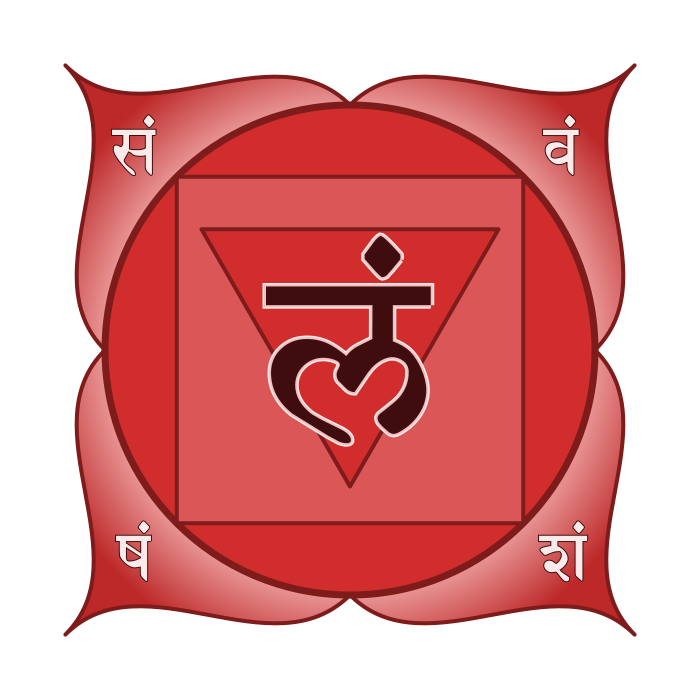
\includegraphics[width=14mm]{images/chakra1}};
    \path[postaction={decorate, decoration={text along path,
      text={|\cardfont\fontsize{7}{8}\selectfont\color{red}|Root},
      text align=center, raise=0pt}}]
      (170:8mm) arc (170:10:8mm);
  \end{scope}%
}

% Moon — purple
\newcommand{\plmoon}{%
  \node[anchor=center, text=purple, font=\symbfont\fontsize{160}{170}\selectfont]
    at (0.5\cardwidth, 0.52\cardheight) {☽};
  \node[anchor=north, text=black, font=\cardfont\fontsize{17}{19}\selectfont]
    at (0.5\cardwidth, 0.52\cardheight-24mm) {Moon};
  \node[anchor=north, text=black, font=\cardfont\fontsize{9}{11}\selectfont]
    at (0.5\cardwidth, \cardheight-6mm) {Luminary of Night};
  \node[anchor=base east, text=black, font=\cardfont\fontsize{9}{11}\selectfont, inner xsep=3mm]
    at (0.5\cardwidth, \cardheight-13mm) {\resizebox{12mm}{\height}{exalted in}};
  \node[anchor=base, text=black, font=\symbserif\fontsize{12}{14}\selectfont]
    at (0.5\cardwidth, \cardheight-13mm) {♉};
  \node[anchor=base west, text=black, font=\cardfont\fontsize{9}{11}\selectfont, inner xsep=3mm]
    at (0.5\cardwidth, \cardheight-13mm) {Taurus};
  \node[anchor=north, text=black, font=\cardfont\fontsize{9}{11}\selectfont]
    at (0.5\cardwidth, 0.52\cardheight-30mm) {Joy in 2\textsuperscript{nd} H. of the Goddess};
  \node[anchor=north, text=black, font=\cardfont\fontsize{17}{19}\selectfont]
    at (0.5\cardwidth, 0.52\cardheight-34mm) {Mystery};
  % 月 Moon / Yin
  \node[anchor=base, text=black, font=\cardfont\fontsize{10}{12}\selectfont]
    at (0.5\cardwidth, 0.52\cardheight-43mm) {yuè};
  \node[anchor=north, text=black, font=\cjkfont\fontsize{18}{20}\selectfont]
    at (0.5\cardwidth, 0.52\cardheight-42.5mm) {月};
  \node[anchor=north, text=black, font=\cardfont\fontsize{10}{12}\selectfont]
    at (0.5\cardwidth, 0.52\cardheight-49mm) {yin};
  \node[anchor=center, text=black, font=\greekfont\fontsize{18}{20}\selectfont]
    at (7mm, 5mm) {Α};
  \begin{scope}[shift={(\cardwidth-9mm,7mm)}]
    \node[anchor=center, inner sep=0pt] at (0,0) {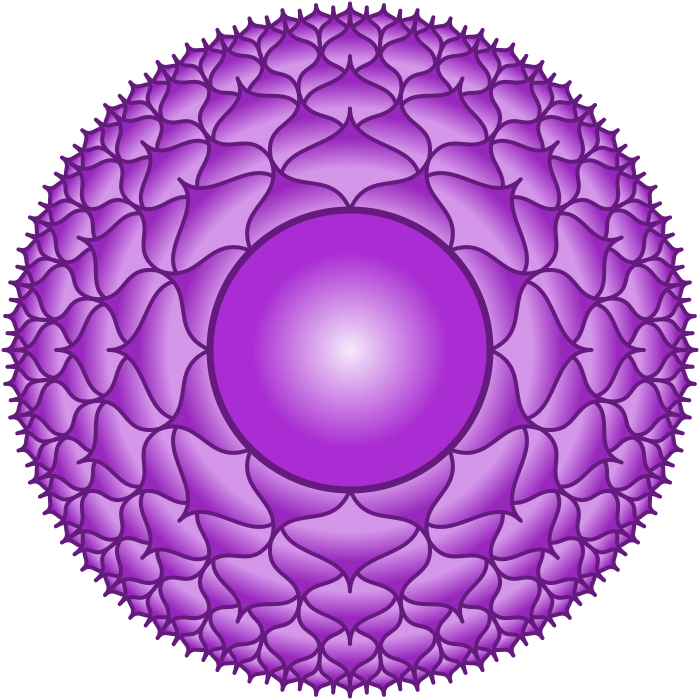
\includegraphics[width=14mm]{images/chakra7}};
    \path[postaction={decorate, decoration={text along path,
      text={|\cardfont\fontsize{7}{8}\selectfont\color{violet}|Crown},
      text align=center, raise=0pt}}]
      (170:8mm) arc (170:10:8mm);
  \end{scope}%
}

% Triplicity rulers: day ruler, night ruler, participating ruler
% Curved "day" and "night" labels above the first two symbols
\newcommand{\triplicityrulers}[3]{%
  % #1=day ruler (font+glyph), #2=night ruler, #3=participating ruler
  \begin{scope}[shift={(0.5\cardwidth, 0.52\cardheight-35.5mm)}]
    % Day ruler
    \node[anchor=center, text=black] at (-10mm, 0) {#1};
    \path[postaction={decorate, decoration={text along path,
      text={|\cardfont\fontsize{7}{8}\selectfont|day},
      text align=center, raise=0pt}}]
      (-14.33mm, 0.5mm) arc (150:30:5mm);
    % Night ruler
    \node[anchor=center, text=black] at (0, 0) {#2};
    \path[postaction={decorate, decoration={text along path,
      text={|\cardfont\fontsize{7}{8}\selectfont|night},
      text align=center, raise=0pt}}]
      (-4.33mm, 0.5mm) arc (150:30:5mm);
    % Participating ruler
    \node[anchor=center, text=black] at (10mm, 0) {#3};
  \end{scope}%
}
% Element-specific triplicity ruler sets (Dorothean)
\newcommand{\firerulers}{\triplicityrulers{{\symbfont\fontsize{14}{16}\selectfont ☉}}{{\symbserif\fontsize{14}{16}\selectfont ♃}}{{\symbserif\fontsize{14}{16}\selectfont ♄}}}
\newcommand{\earthrulers}{\triplicityrulers{{\symbserif\fontsize{14}{16}\selectfont ♀}}{{\symbfont\fontsize{14}{16}\selectfont ☽}}{{\symbserif\fontsize{14}{16}\selectfont ♂}}}
\newcommand{\airrulers}{\triplicityrulers{{\symbserif\fontsize{14}{16}\selectfont ♄}}{{\symbserif\fontsize{14}{16}\selectfont ☿}}{{\symbserif\fontsize{14}{16}\selectfont ♃}}}
\newcommand{\waterrulers}{\triplicityrulers{{\symbserif\fontsize{14}{16}\selectfont ♀}}{{\symbserif\fontsize{14}{16}\selectfont ♂}}{{\symbfont\fontsize{14}{16}\selectfont ☽}}}

% Small planet symbols for ruler rows
\newcommand{\rSun}{{\symbfont\fontsize{14}{16}\selectfont ☉}}
\newcommand{\rMoon}{{\symbfont\fontsize{14}{16}\selectfont ☽}}
\newcommand{\rMercury}{{\symbserif\fontsize{14}{16}\selectfont ☿}}
\newcommand{\rVenus}{{\symbserif\fontsize{14}{16}\selectfont ♀}}
\newcommand{\rMars}{{\symbserif\fontsize{14}{16}\selectfont ♂}}
\newcommand{\rJupiter}{{\symbserif\fontsize{14}{16}\selectfont ♃}}
\newcommand{\rSaturn}{{\symbserif\fontsize{14}{16}\selectfont ♄}}

% Decan rulers (Chaldean order): three planet symbols in a row
\newcommand{\decanrulers}[3]{%
  \begin{scope}[shift={(0.5\cardwidth, 0.52\cardheight-41.5mm)}]
    \node[anchor=center, text=black] at (-10mm, 0) {#1};
    \node[anchor=center, text=black] at (0, 0) {#2};
    \node[anchor=center, text=black] at (10mm, 0) {#3};
    % Degree ranges curved below each symbol
    \path[postaction={decorate, decoration={text along path,
      text={|\cardfont\fontsize{7}{8}\selectfont|0-10},
      text align=center, raise=0pt}}]
      (-15.2mm, -1mm) arc (210:330:6mm);
    \path[postaction={decorate, decoration={text along path,
      text={|\cardfont\fontsize{7}{8}\selectfont|10-20},
      text align=center, raise=0pt}}]
      (-5.2mm, -1mm) arc (210:330:6mm);
    \path[postaction={decorate, decoration={text along path,
      text={|\cardfont\fontsize{7}{8}\selectfont|20-30},
      text align=center, raise=0pt}}]
      (4.8mm, -1mm) arc (210:330:6mm);
  \end{scope}%
}

% Tidal hexagram (消息卦) — drawn centered on card edge, clipped to half
% #1=x, #2=y (center), #3=line pattern, #4=phonetic, #5=english
\newcommand{\drawhexagram}[8]{%
  \begin{scope}[shift={(#1, #2)}, line width=1.5mm, line cap=butt]
    \foreach \type [count=\i from 0] in {#3} {
      \ifnum\type=1
        \draw (-6mm, \i*4mm-10mm) -- (6mm, \i*4mm-10mm);
      \else
        \draw (-6mm, \i*4mm-10mm) -- (-2mm, \i*4mm-10mm);
        \draw (2mm, \i*4mm-10mm) -- (6mm, \i*4mm-10mm);
      \fi
    }
    \node[anchor=south, text=black, font=\cardfont\fontsize{8}{9}\selectfont]
      at (0, 13mm) {#4};
    \node[anchor=north, text=black, font=\cardfont\fontsize{8}{9}\selectfont]
      at (0, -13mm) {#5};
    % Earthly branch
    \node[anchor=base, text=black, font=\cardfont\fontsize{7}{8}\selectfont]
      at (0, -21mm) {#6};
    \node[anchor=north, text=black, font=\cjkfont\fontsize{11}{13}\selectfont]
      at (0, -21.5mm) {#7};
    \node[anchor=north, text=black, font=\cardfont\fontsize{7}{8}\selectfont]
      at (0, -26mm) {#8};
  \end{scope}%
}

% 24 Solar Terms (二十四节气) — two per zodiac sign
% #1=left kanji, #2=left pinyin, #3=left english
% #4=right kanji, #5=right pinyin, #6=right english
% #7=left animal color, #8=right animal color
\newcommand{\solarterms}[8]{%
  % Season animal indicator line at bottom
  \fill[#7] (0, 0) rectangle (0.5\cardwidth, 0.75mm);
  \fill[#8] (0.5\cardwidth, 0) rectangle (\cardwidth, 0.75mm);
  % Left solar term (0°)
  \node[anchor=base west, text=black, font=\cjkfont\fontsize{9}{11}\selectfont]
    at (0.5mm, 7.5mm) {#1};
  \node[anchor=base west, text=black, font=\cardfont\fontsize{7}{8}\selectfont]
    at (0.5mm, 4.5mm) {#2};
  \node[anchor=base west, text=black, font=\cardfont\fontsize{7}{8}\selectfont]
    at (0.5mm, 1.5mm) {#3};
  % Right solar term (15°)
  \node[anchor=base east, text=black, font=\cjkfont\fontsize{9}{11}\selectfont]
    at (\cardwidth-0.5mm, 7.5mm) {#4};
  \node[anchor=base east, text=black, font=\cardfont\fontsize{7}{8}\selectfont]
    at (\cardwidth-0.5mm, 4.5mm) {#5};
  \node[anchor=base east, text=black, font=\cardfont\fontsize{7}{8}\selectfont]
    at (\cardwidth-0.5mm, 1.5mm) {#6};
}

% Zodiac sign overlays
% Aries (Emperor) — Red — Domicile of Mars
\newcommand{\zdaries}{%
  \node[anchor=center, text=red, font=\symbserif\fontsize{160}{170}\selectfont]
    at (0.5\cardwidth, 0.52\cardheight) {♈};
  \node[anchor=north, text=black, font=\cardfont\fontsize{17}{19}\selectfont]
    at (0.5\cardwidth, 0.52\cardheight-24mm) {Aries};
  \node[anchor=base east, text=black, font=\cardfont\fontsize{9}{11}\selectfont, inner xsep=3mm]
    at (0.5\cardwidth, \cardheight-10mm) {\resizebox{12mm}{\height}{Domicile of}};
  \node[anchor=base, text=black, font=\symbserif\fontsize{12}{14}\selectfont]
    at (0.5\cardwidth, \cardheight-10mm) {♂};
  \node[anchor=base west, text=black, font=\cardfont\fontsize{9}{11}\selectfont, inner xsep=3mm]
    at (0.5\cardwidth, \cardheight-10mm) {Mars};
  \node[anchor=north, text=black, font=\cardfont\fontsize{9}{11}\selectfont]
    at (0.5\cardwidth, \cardheight-10mm) {cardinal fire};
  \node[anchor=center, text=black] at (0.5\cardwidth-3.5mm, \cardheight-16mm) {\tinysulfur};
  \node[anchor=center, text=black] at (0.5\cardwidth+3.5mm, \cardheight-16mm) {\tinyfire};
  \firerulers
  \decanrulers{\rMars}{\rSun}{\rVenus}
  \solarterms{春分}{Chūnfēn}{Spring Equinox}{清明}{Qīngmíng}{Clear \& Bright}{blue}{blue}
  \drawhexagram{0}{0.5\cardheight}{1,1,1,1,0,0}{Dàzhuàng}{Great Strength}{Mǎo}{卯}{Rabbit}% 大壮 Pisces→Aries
  \drawhexagram{\cardwidth}{0.5\cardheight}{1,1,1,1,1,0}{Guài}{Breakthrough}{Chén}{辰}{Dragon}% 夬 Aries→Taurus
}
% Taurus (Hierophant) — Red-Orange — Domicile of Venus
\newcommand{\zdtaurus}{%
  \node[anchor=center, text=red!50!orange, font=\symbserif\fontsize{160}{170}\selectfont]
    at (0.5\cardwidth, 0.52\cardheight) {♉};
  \node[anchor=north, text=black, font=\cardfont\fontsize{17}{19}\selectfont]
    at (0.5\cardwidth, 0.52\cardheight-24mm) {Taurus};
  \node[anchor=base east, text=black, font=\cardfont\fontsize{9}{11}\selectfont, inner xsep=3mm]
    at (0.5\cardwidth, \cardheight-10mm) {\resizebox{12mm}{\height}{Domicile of}};
  \node[anchor=base, text=black, font=\symbserif\fontsize{12}{14}\selectfont]
    at (0.5\cardwidth, \cardheight-10mm) {♀};
  \node[anchor=base west, text=black, font=\cardfont\fontsize{9}{11}\selectfont, inner xsep=3mm]
    at (0.5\cardwidth, \cardheight-10mm) {Venus};
  \node[anchor=north, text=black, font=\cardfont\fontsize{9}{11}\selectfont]
    at (0.5\cardwidth, \cardheight-10mm) {fixed earth};
  \node[anchor=center, text=black] at (0.5\cardwidth-3.5mm, \cardheight-16mm) {\tinysalt};
  \node[anchor=center, text=black] at (0.5\cardwidth+3.5mm, \cardheight-16mm) {\tinyearth};
  \earthrulers
  \decanrulers{\rMercury}{\rMoon}{\rSaturn}
  \solarterms{谷雨}{Gǔyǔ}{Grain Rain}{立夏}{Lìxià}{Start of Summer}{blue}{red}
  \drawhexagram{0}{0.5\cardheight}{1,1,1,1,1,0}{Guài}{Breakthrough}{Chén}{辰}{Dragon}% 夬 Aries→Taurus
  \drawhexagram{\cardwidth}{0.5\cardheight}{1,1,1,1,1,1}{Qián}{Heaven}{Sì}{巳}{Snake}% 乾 Taurus→Gemini
}
% Gemini (Lovers) — Orange — Domicile of Mercury
\newcommand{\zdgemini}{%
  \node[anchor=center, text=orange, font=\symbserif\fontsize{160}{170}\selectfont]
    at (0.5\cardwidth, 0.52\cardheight) {♊};
  \node[anchor=north, text=black, font=\cardfont\fontsize{17}{19}\selectfont]
    at (0.5\cardwidth, 0.52\cardheight-24mm) {Gemini};
  \node[anchor=base east, text=black, font=\cardfont\fontsize{9}{11}\selectfont, inner xsep=3mm]
    at (0.5\cardwidth, \cardheight-10mm) {\resizebox{12mm}{\height}{Domicile of}};
  \node[anchor=base, text=black, font=\symbserif\fontsize{12}{14}\selectfont]
    at (0.5\cardwidth, \cardheight-10mm) {☿};
  \node[anchor=base west, text=black, font=\cardfont\fontsize{9}{11}\selectfont, inner xsep=3mm]
    at (0.5\cardwidth, \cardheight-10mm) {Mercury};
  \node[anchor=north, text=black, font=\cardfont\fontsize{9}{11}\selectfont]
    at (0.5\cardwidth, \cardheight-10mm) {mutable air};
  \node[anchor=center, text=black] at (0.5\cardwidth-3.5mm, \cardheight-16mm) {\tinymercury};
  \node[anchor=center, text=black] at (0.5\cardwidth+3.5mm, \cardheight-16mm) {\tinyair};
  \airrulers
  \decanrulers{\rJupiter}{\rMars}{\rSun}
  \solarterms{小满}{Xiǎomǎn}{Grain Buds}{芒种}{Mángzhòng}{Grain in Ear}{red}{red}
  \drawhexagram{0}{0.5\cardheight}{1,1,1,1,1,1}{Qián}{Heaven}{Sì}{巳}{Snake}% 乾 Taurus→Gemini
  \drawhexagram{\cardwidth}{0.5\cardheight}{0,1,1,1,1,1}{Gòu}{Encounter}{Wǔ}{午}{Horse}% 姤 Gemini→Cancer
}
% Cancer (Chariot) — Amber — Domicile of Moon
\newcommand{\zdcancer}{%
  \node[anchor=center, text=yellow!50!orange, font=\symbserif\fontsize{160}{170}\selectfont]
    at (0.5\cardwidth, 0.52\cardheight) {♋};
  \node[anchor=north, text=black, font=\cardfont\fontsize{17}{19}\selectfont]
    at (0.5\cardwidth, 0.52\cardheight-24mm) {Cancer};
  \node[anchor=base east, text=black, font=\cardfont\fontsize{9}{11}\selectfont, inner xsep=3mm]
    at (0.5\cardwidth, \cardheight-10mm) {\resizebox{12mm}{\height}{Domicile of}};
  \node[anchor=base, text=black, font=\symbfont\fontsize{12}{14}\selectfont]
    at (0.5\cardwidth, \cardheight-10mm) {☽};
  \node[anchor=base west, text=black, font=\cardfont\fontsize{9}{11}\selectfont, inner xsep=3mm]
    at (0.5\cardwidth, \cardheight-10mm) {Moon};
  \node[anchor=north, text=black, font=\cardfont\fontsize{9}{11}\selectfont]
    at (0.5\cardwidth, \cardheight-10mm) {cardinal water};
  \node[anchor=center, text=black] at (0.5\cardwidth-3.5mm, \cardheight-16mm) {\tinysulfur};
  \node[anchor=center, text=black] at (0.5\cardwidth+3.5mm, \cardheight-16mm) {\tinywater};
  \waterrulers
  \decanrulers{\rVenus}{\rMercury}{\rMoon}
  \solarterms{夏至}{Xiàzhì}{Summer Solstice}{小暑}{Xiǎoshǔ}{Minor Heat}{red}{red}
  \drawhexagram{0}{0.5\cardheight}{0,1,1,1,1,1}{Gòu}{Encounter}{Wǔ}{午}{Horse}% 姤 Gemini→Cancer
  \drawhexagram{\cardwidth}{0.5\cardheight}{0,0,1,1,1,1}{Dùn}{Retreat}{Wèi}{未}{Goat}% 遯 Cancer→Leo
}
% Leo (Strength) — Yellow — Domicile of Sun
\newcommand{\zdleo}{%
  \node[anchor=center, text=yellow!80!orange, font=\symbserif\fontsize{160}{170}\selectfont]
    at (0.5\cardwidth, 0.52\cardheight) {♌};
  \node[anchor=north, text=black, font=\cardfont\fontsize{17}{19}\selectfont]
    at (0.5\cardwidth, 0.52\cardheight-24mm) {Leo};
  \node[anchor=base east, text=black, font=\cardfont\fontsize{9}{11}\selectfont, inner xsep=3mm]
    at (0.5\cardwidth, \cardheight-10mm) {\resizebox{12mm}{\height}{Domicile of}};
  \node[anchor=base, text=black, font=\symbfont\fontsize{12}{14}\selectfont]
    at (0.5\cardwidth, \cardheight-10mm) {☉};
  \node[anchor=base west, text=black, font=\cardfont\fontsize{9}{11}\selectfont, inner xsep=3mm]
    at (0.5\cardwidth, \cardheight-10mm) {Sun};
  \node[anchor=north, text=black, font=\cardfont\fontsize{9}{11}\selectfont]
    at (0.5\cardwidth, \cardheight-10mm) {fixed fire};
  \node[anchor=center, text=black] at (0.5\cardwidth-3.5mm, \cardheight-16mm) {\tinysalt};
  \node[anchor=center, text=black] at (0.5\cardwidth+3.5mm, \cardheight-16mm) {\tinyfire};
  \firerulers
  \decanrulers{\rSaturn}{\rJupiter}{\rMars}
  \solarterms{大暑}{Dàshǔ}{Major Heat}{立秋}{Lìqiū}{Start of Autumn}{red}{white}
  \drawhexagram{0}{0.5\cardheight}{0,0,1,1,1,1}{Dùn}{Retreat}{Wèi}{未}{Goat}% 遯 Cancer→Leo
  \drawhexagram{\cardwidth}{0.5\cardheight}{0,0,0,1,1,1}{Pǐ}{Stagnation}{Shēn}{申}{Monkey}% 否 Leo→Virgo
}
% Virgo (Hermit) — Yellow-Green — Domicile of Mercury
\newcommand{\zdvirgo}{%
  \node[anchor=center, text=yellow!50!green, font=\symbserif\fontsize{160}{170}\selectfont,
    xscale=0.78] at (0.5\cardwidth, 0.52\cardheight) {♍};
  \node[anchor=north, text=black, font=\cardfont\fontsize{17}{19}\selectfont]
    at (0.5\cardwidth, 0.52\cardheight-24mm) {Virgo};
  \node[anchor=base east, text=black, font=\cardfont\fontsize{9}{11}\selectfont, inner xsep=3mm]
    at (0.5\cardwidth, \cardheight-10mm) {\resizebox{12mm}{\height}{Domicile of}};
  \node[anchor=base, text=black, font=\symbserif\fontsize{12}{14}\selectfont]
    at (0.5\cardwidth, \cardheight-10mm) {☿};
  \node[anchor=base west, text=black, font=\cardfont\fontsize{9}{11}\selectfont, inner xsep=3mm]
    at (0.5\cardwidth, \cardheight-10mm) {Mercury};
  \node[anchor=north, text=black, font=\cardfont\fontsize{9}{11}\selectfont]
    at (0.5\cardwidth, \cardheight-10mm) {mutable earth};
  \node[anchor=center, text=black] at (0.5\cardwidth-3.5mm, \cardheight-16mm) {\tinymercury};
  \node[anchor=center, text=black] at (0.5\cardwidth+3.5mm, \cardheight-16mm) {\tinyearth};
  \earthrulers
  \decanrulers{\rSun}{\rVenus}{\rMercury}
  \solarterms{处暑}{Chǔshǔ}{End of Heat}{白露}{Báilù}{White Dew}{white}{white}
  \drawhexagram{0}{0.5\cardheight}{0,0,0,1,1,1}{Pǐ}{Stagnation}{Shēn}{申}{Monkey}% 否 Leo→Virgo
  \drawhexagram{\cardwidth}{0.5\cardheight}{0,0,0,0,1,1}{Guān}{Contemplation}{Yǒu}{酉}{Rooster}% 观 Virgo→Libra
}
% Libra (Justice) — Green — Domicile of Venus
\newcommand{\zdlibra}{%
  \node[anchor=center, text=green!70!black, font=\symbserif\fontsize{160}{170}\selectfont]
    at (0.5\cardwidth, 0.52\cardheight) {♎};
  \node[anchor=north, text=black, font=\cardfont\fontsize{17}{19}\selectfont]
    at (0.5\cardwidth, 0.52\cardheight-24mm) {Libra};
  \node[anchor=base east, text=black, font=\cardfont\fontsize{9}{11}\selectfont, inner xsep=3mm]
    at (0.5\cardwidth, \cardheight-10mm) {\resizebox{12mm}{\height}{Domicile of}};
  \node[anchor=base, text=black, font=\symbserif\fontsize{12}{14}\selectfont]
    at (0.5\cardwidth, \cardheight-10mm) {♀};
  \node[anchor=base west, text=black, font=\cardfont\fontsize{9}{11}\selectfont, inner xsep=3mm]
    at (0.5\cardwidth, \cardheight-10mm) {Venus};
  \node[anchor=north, text=black, font=\cardfont\fontsize{9}{11}\selectfont]
    at (0.5\cardwidth, \cardheight-10mm) {cardinal air};
  \node[anchor=center, text=black] at (0.5\cardwidth-3.5mm, \cardheight-16mm) {\tinysulfur};
  \node[anchor=center, text=black] at (0.5\cardwidth+3.5mm, \cardheight-16mm) {\tinyair};
  \airrulers
  \decanrulers{\rMoon}{\rSaturn}{\rJupiter}
  \solarterms{秋分}{Qiūfēn}{Autumn Equinox}{寒露}{Hánlù}{Cold Dew}{white}{white}
  \drawhexagram{0}{0.5\cardheight}{0,0,0,0,1,1}{Guān}{Contemplation}{Yǒu}{酉}{Rooster}% 观 Virgo→Libra
  \drawhexagram{\cardwidth}{0.5\cardheight}{0,0,0,0,0,1}{Bō}{Splitting\\Apart}{Xū}{戌}{Dog}% 剥 Libra→Scorpio
}
% Scorpio (Death) — Turquoise — Domicile of Mars
\newcommand{\zdscorpio}{%
  \node[anchor=center, text=blue!50!green, font=\symbserif\fontsize{160}{170}\selectfont,
    xscale=0.73] at (0.5\cardwidth, 0.52\cardheight) {♏};
  \node[anchor=north, text=black, font=\cardfont\fontsize{17}{19}\selectfont]
    at (0.5\cardwidth, 0.52\cardheight-24mm) {Scorpio};
  \node[anchor=base east, text=black, font=\cardfont\fontsize{9}{11}\selectfont, inner xsep=3mm]
    at (0.5\cardwidth, \cardheight-10mm) {\resizebox{12mm}{\height}{Domicile of}};
  \node[anchor=base, text=black, font=\symbserif\fontsize{12}{14}\selectfont]
    at (0.5\cardwidth, \cardheight-10mm) {♂};
  \node[anchor=base west, text=black, font=\cardfont\fontsize{9}{11}\selectfont, inner xsep=3mm]
    at (0.5\cardwidth, \cardheight-10mm) {Mars};
  \node[anchor=north, text=black, font=\cardfont\fontsize{9}{11}\selectfont]
    at (0.5\cardwidth, \cardheight-10mm) {fixed water};
  \node[anchor=center, text=black] at (0.5\cardwidth-3.5mm, \cardheight-16mm) {\tinysalt};
  \node[anchor=center, text=black] at (0.5\cardwidth+3.5mm, \cardheight-16mm) {\tinywater};
  \waterrulers
  \decanrulers{\rMars}{\rSun}{\rVenus}
  \solarterms{霜降}{Shuāngjiàng}{Frost's Descent}{立冬}{Lìdōng}{Start of Winter}{white}{black}
  \drawhexagram{0}{0.5\cardheight}{0,0,0,0,0,1}{Bō}{Splitting\\Apart}{Xū}{戌}{Dog}% 剥 Libra→Scorpio
  \drawhexagram{\cardwidth}{0.5\cardheight}{0,0,0,0,0,0}{Kūn}{Earth}{Hài}{亥}{Pig}% 坤 Scorpio→Sagittarius
}
% Sagittarius (Temperance) — Blue — Domicile of Jupiter
\newcommand{\zdsagittarius}{%
  \node[anchor=center, text=blue, font=\symbserif\fontsize{160}{170}\selectfont]
    at (0.5\cardwidth, 0.52\cardheight) {♐};
  \node[anchor=north, text=black, font=\cardfont\fontsize{17}{19}\selectfont]
    at (0.5\cardwidth, 0.52\cardheight-24mm) {Sagittarius};
  \node[anchor=base east, text=black, font=\cardfont\fontsize{9}{11}\selectfont, inner xsep=3mm]
    at (0.5\cardwidth, \cardheight-10mm) {\resizebox{12mm}{\height}{Domicile of}};
  \node[anchor=base, text=black, font=\symbserif\fontsize{12}{14}\selectfont]
    at (0.5\cardwidth, \cardheight-10mm) {♃};
  \node[anchor=base west, text=black, font=\cardfont\fontsize{9}{11}\selectfont, inner xsep=3mm]
    at (0.5\cardwidth, \cardheight-10mm) {Jupiter};
  \node[anchor=north, text=black, font=\cardfont\fontsize{9}{11}\selectfont]
    at (0.5\cardwidth, \cardheight-10mm) {mutable fire};
  \node[anchor=center, text=black] at (0.5\cardwidth-3.5mm, \cardheight-16mm) {\tinymercury};
  \node[anchor=center, text=black] at (0.5\cardwidth+3.5mm, \cardheight-16mm) {\tinyfire};
  \firerulers
  \decanrulers{\rMercury}{\rMoon}{\rSaturn}
  \solarterms{小雪}{Xiǎoxuě}{Minor Snow}{大雪}{Dàxuě}{Major Snow}{black}{black}
  \drawhexagram{0}{0.5\cardheight}{0,0,0,0,0,0}{Kūn}{Earth}{Hài}{亥}{Pig}% 坤 Scorpio→Sagittarius
  \drawhexagram{\cardwidth}{0.5\cardheight}{1,0,0,0,0,0}{Fù}{Return}{Zǐ}{子}{Rat}% 复 Sagittarius→Capricorn
}
% Capricorn (Devil) — Indigo — Domicile of Saturn
\newcommand{\zdcapricorn}{%
  \node[anchor=center, text=blue!50!violet, font=\symbserif\fontsize{160}{170}\selectfont]
    at (0.5\cardwidth, 0.52\cardheight) {♑};
  \node[anchor=north, text=black, font=\cardfont\fontsize{17}{19}\selectfont]
    at (0.5\cardwidth, 0.52\cardheight-24mm) {Capricorn};
  \node[anchor=base east, text=black, font=\cardfont\fontsize{9}{11}\selectfont, inner xsep=3mm]
    at (0.5\cardwidth, \cardheight-10mm) {\resizebox{12mm}{\height}{Domicile of}};
  \node[anchor=base, text=black, font=\symbserif\fontsize{12}{14}\selectfont]
    at (0.5\cardwidth, \cardheight-10mm) {♄};
  \node[anchor=base west, text=black, font=\cardfont\fontsize{9}{11}\selectfont, inner xsep=3mm]
    at (0.5\cardwidth, \cardheight-10mm) {Saturn};
  \node[anchor=north, text=black, font=\cardfont\fontsize{9}{11}\selectfont]
    at (0.5\cardwidth, \cardheight-10mm) {cardinal earth};
  \node[anchor=center, text=black] at (0.5\cardwidth-3.5mm, \cardheight-16mm) {\tinysulfur};
  \node[anchor=center, text=black] at (0.5\cardwidth+3.5mm, \cardheight-16mm) {\tinyearth};
  \earthrulers
  \decanrulers{\rJupiter}{\rMars}{\rSun}
  \solarterms{冬至}{Dōngzhì}{Winter Solstice}{小寒}{Xiǎohán}{Minor Cold}{black}{black}
  \drawhexagram{0}{0.5\cardheight}{1,0,0,0,0,0}{Fù}{Return}{Zǐ}{子}{Rat}% 复 Sagittarius→Capricorn
  \drawhexagram{\cardwidth}{0.5\cardheight}{1,1,0,0,0,0}{Lín}{Approach}{Chǒu}{丑}{Ox}% 临 Capricorn→Aquarius
}
% Aquarius (Star) — Violet — Domicile of Saturn
\newcommand{\zdaquarius}{%
  \node[anchor=center, text=violet, font=\symbserif\fontsize{160}{170}\selectfont]
    at (0.5\cardwidth, 0.52\cardheight) {♒};
  \node[anchor=north, text=black, font=\cardfont\fontsize{17}{19}\selectfont]
    at (0.5\cardwidth, 0.52\cardheight-24mm) {Aquarius};
  \node[anchor=base east, text=black, font=\cardfont\fontsize{9}{11}\selectfont, inner xsep=3mm]
    at (0.5\cardwidth, \cardheight-10mm) {\resizebox{12mm}{\height}{Domicile of}};
  \node[anchor=base, text=black, font=\symbserif\fontsize{12}{14}\selectfont]
    at (0.5\cardwidth, \cardheight-10mm) {♄};
  \node[anchor=base west, text=black, font=\cardfont\fontsize{9}{11}\selectfont, inner xsep=3mm]
    at (0.5\cardwidth, \cardheight-10mm) {Saturn};
  \node[anchor=north, text=black, font=\cardfont\fontsize{9}{11}\selectfont]
    at (0.5\cardwidth, \cardheight-10mm) {fixed air};
  \node[anchor=center, text=black] at (0.5\cardwidth-3.5mm, \cardheight-16mm) {\tinysalt};
  \node[anchor=center, text=black] at (0.5\cardwidth+3.5mm, \cardheight-16mm) {\tinyair};
  \airrulers
  \decanrulers{\rVenus}{\rMercury}{\rMoon}
  \solarterms{大寒}{Dàhán}{Major Cold}{立春}{Lìchūn}{Start of Spring}{black}{blue}
  \drawhexagram{0}{0.5\cardheight}{1,1,0,0,0,0}{Lín}{Approach}{Chǒu}{丑}{Ox}% 临 Capricorn→Aquarius
  \drawhexagram{\cardwidth}{0.5\cardheight}{1,1,1,0,0,0}{Tài}{Peace}{Yín}{寅}{Tiger}% 泰 Aquarius→Pisces
}
% Pisces (Moon XVIII) — Red-Violet — Domicile of Jupiter
\newcommand{\zdpisces}{%
  \node[anchor=center, text=red!50!violet, font=\symbserif\fontsize{160}{170}\selectfont]
    at (0.5\cardwidth, 0.52\cardheight) {♓};
  \node[anchor=north, text=black, font=\cardfont\fontsize{17}{19}\selectfont]
    at (0.5\cardwidth, 0.52\cardheight-24mm) {Pisces};
  \node[anchor=base east, text=black, font=\cardfont\fontsize{9}{11}\selectfont, inner xsep=3mm]
    at (0.5\cardwidth, \cardheight-10mm) {\resizebox{12mm}{\height}{Domicile of}};
  \node[anchor=base, text=black, font=\symbserif\fontsize{12}{14}\selectfont]
    at (0.5\cardwidth, \cardheight-10mm) {♃};
  \node[anchor=base west, text=black, font=\cardfont\fontsize{9}{11}\selectfont, inner xsep=3mm]
    at (0.5\cardwidth, \cardheight-10mm) {Jupiter};
  \node[anchor=north, text=black, font=\cardfont\fontsize{9}{11}\selectfont]
    at (0.5\cardwidth, \cardheight-10mm) {mutable water};
  \node[anchor=center, text=black] at (0.5\cardwidth-3.5mm, \cardheight-16mm) {\tinymercury};
  \node[anchor=center, text=black] at (0.5\cardwidth+3.5mm, \cardheight-16mm) {\tinywater};
  \waterrulers
  \decanrulers{\rSaturn}{\rJupiter}{\rMars}
  \solarterms{雨水}{Yǔshuǐ}{Rain Water}{惊蛰}{Jīngzhé}{Awakening of Insects}{blue}{blue}
  \drawhexagram{0}{0.5\cardheight}{1,1,1,0,0,0}{Tài}{Peace}{Yín}{寅}{Tiger}% 泰 Aquarius→Pisces
  \drawhexagram{\cardwidth}{0.5\cardheight}{1,1,1,1,0,0}{Dàzhuàng}{Great Strength}{Mǎo}{卯}{Rabbit}% 大壮 Pisces→Aries
}

% Small hexagram for ace cards — compact version of \drawhexagram
\newcommand{\drawsmallhexagram}[5]{%
  \begin{scope}[shift={(#1, #2)}, line width=1.2mm, line cap=butt]
    \foreach \type [count=\i from 0] in {#3} {
      \ifnum\type=1
        \draw (-5mm, \i*2.5mm-6.25mm) -- (5mm, \i*2.5mm-6.25mm);
      \else
        \draw (-5mm, \i*2.5mm-6.25mm) -- (-1.5mm, \i*2.5mm-6.25mm);
        \draw (1.5mm, \i*2.5mm-6.25mm) -- (5mm, \i*2.5mm-6.25mm);
      \fi
    }
    \node[anchor=south, text=black, font=\cardfont\fontsize{8}{9}\selectfont]
      at (0, 6mm) {#4};
    \node[anchor=north, text=black, font=\cardfont\fontsize{8}{9}\selectfont]
      at (0, -7mm) {#5};
  \end{scope}%
}

% Geomancy figure — 4 rows of 1 or 2 black diamonds
% Small geomancy figure for Aces
% #1 = x, #2 = y, #3 = comma-separated rows (1 or 2, top to bottom), #4 = label below
\newcommand{\drawsmallgeomancy}[4]{%
  \begin{scope}[shift={(#1, #2)}]
    \foreach \dots [count=\i from 0] in {#3} {
      \ifnum\dots=1
        \node[fill=black, inner sep=0.8mm, rotate=45] at (0, -\i*3.5mm) {};
      \else
        \node[fill=black, inner sep=0.8mm, rotate=45] at (-2mm, -\i*3.5mm) {};
        \node[fill=black, inner sep=0.8mm, rotate=45] at (2mm, -\i*3.5mm) {};
      \fi
    }
    \node[anchor=north, text=black, font=\cardfont\fontsize{7}{9}\selectfont]
      at (0, -3*3.5mm-1mm) {#4};
  \end{scope}%
}

% Geomancy figure for court cards
% #1 = x, #2 = y, #3 = comma-separated rows (1 or 2, top to bottom), #4 = label below
\newcommand{\drawgeomancy}[4]{%
  \begin{scope}[shift={(#1, #2)}]
    \foreach \dots [count=\i from 0] in {#3} {
      \ifnum\dots=1
        \node[fill=black, inner sep=2.5mm, rotate=45] at (0, -\i*11mm) {};
      \else
        \node[fill=black, inner sep=2.5mm, rotate=45] at (-6mm, -\i*11mm) {};
        \node[fill=black, inner sep=2.5mm, rotate=45] at (6mm, -\i*11mm) {};
      \fi
    }
    \node[anchor=north, text=black, font=\cardfont\fontsize{17}{19}\selectfont]
      at (0, 0.52\cardheight-24mm-#2) {#4};
  \end{scope}%
}

% Chakra seed syllable stack — vertical column along left edge
% #1 = which chakra to highlight (1=Root/Saturn .. 7=Crown/Moon)
% Draws bottom-to-top: 1=Root at bottom, 7=Crown at top
\newcommand{\chakrastack}[1]{%
  \foreach \syllable [count=\i from 1] in {लं,वं,रं,यं,हं,ॐ} {
    \ifnum\i=#1
      \node[anchor=center, text=black, font=\devfont\bfseries\fontsize{16}{18}\selectfont]
        at (3mm, 0.3\cardheight+\i*5mm) {\syllable};
    \else
      \node[anchor=center, text=black, font=\devfont\fontsize{10}{12}\selectfont]
        at (3mm, 0.3\cardheight+\i*5mm) {\syllable};
    \fi
  }
  % Crown chakra — Devanagari zero
  \ifnum#1=7
    \node[anchor=center, text=black, font=\devfont\bfseries\fontsize{22}{24}\selectfont]
      at (3mm, 0.3\cardheight+35mm) {०};
  \else
    \node[anchor=center, text=black, font=\devfont\fontsize{10}{12}\selectfont]
      at (3mm, 0.3\cardheight+35mm) {०};
  \fi
  % English chakra label, rotated 90°
  \def\chakraord{\ifcase#1\or 1st\or 2nd\or 3rd\or 4th\or 5th\or 6th\or 7th\fi}%
  \def\chakraname{\ifcase#1\or Root\or Sacral\or Solar Plexus\or Heart\or Throat\or Third Eye\or Crown\fi}%
  \node[anchor=center, text=black, font=\cardfont\fontsize{7}{9}\selectfont, rotate=90]
    at (7mm, 0.3\cardheight+20mm) {\chakraord{} Chakra - \chakraname};
}

% Lunar stack — sun at bottom, 7 crescents above (bright sides toward sun)
% #1 = chakra/gate number (1=root/closest to sun..7=crown/furthest), #2 = "removes" or "reclaims"
\newcommand{\lunarstack}[2]{%
  \newcount\activegate\activegate=#1\relax
  \def\isdescending{removes}\def\direction{#2}%
  % 8 evenly spaced symbols: sun at position 0, moons at positions 1-7
  \node[anchor=center, text=black, font=\symbserif\fontsize{10}{12}\selectfont]
    at (\cardwidth-3mm, 0.3\cardheight+5mm) {☉};
  \foreach \i in {1,...,7} {
    \ifnum\i=\activegate
      \node[anchor=center, text=black, font=\symbserif\fontsize{11}{13}\selectfont, rotate=-90]
        at (\cardwidth-3mm, 0.3\cardheight+5mm+\i*4.3mm) {☽};
    \else
      \node[anchor=center, text=black, font=\symbserif\fontsize{8}{10}\selectfont, rotate=-90]
        at (\cardwidth-3mm, 0.3\cardheight+5mm+\i*4.3mm) {☽};
    \fi
  }
  % Arrow at the active gate — drawn outside loop to avoid expansion issues
  \ifx\direction\isdescending
    \draw[->, thick] (\cardwidth-3mm, 0.3\cardheight+5mm+#1*4.3mm+0.5mm) -- ++(0, -3mm);
  \else
    \draw[->, thick] (\cardwidth-3mm, 0.3\cardheight+5mm+#1*4.3mm-1.5mm) -- ++(0, 3mm);
  \fi
  % Inanna's gate text — removes reads top-to-bottom, reclaims reads bottom-to-top
  \def\inannaitem{\ifcase#1\or robe\or anklet\or ring\or breastplate\or lapis necklace\or royal staff\or crown\fi}%
  \ifx\direction\isdescending
    \node[anchor=center, text=black, font=\cardfont\fontsize{7}{9}\selectfont, rotate=-90]
      at (\cardwidth-7mm, 0.3\cardheight+20mm) {{\cuneiform 𒈹} #2 her \inannaitem};
  \else
    \node[anchor=center, text=black, font=\cardfont\fontsize{7}{9}\selectfont, rotate=90]
      at (\cardwidth-7mm, 0.3\cardheight+20mm) {{\cuneiform 𒈹} #2 her \inannaitem};
  \fi
}

% Moon phase diagram — draws a circle showing the lunar phase
% #1 = x, #2 = y, #3 = phase (0=new, 4=first quarter, 8=full, 12=third quarter)
\newcommand{\drawmoonphase}[3]{%
  \begin{scope}[shift={(#1,#2)}]
    \pgfmathtruncatemacro{\p}{#3}%
    \fill[black!80] (0,0) circle (3mm);
    \ifnum\p=8
      \fill[white] (0,0) circle (3mm);
    \fi
    \ifnum\p>0 \ifnum\p<8
      % Waxing: right side lit
      \pgfmathsetmacro{\tx}{3 * cos(\p * 22.5)}%
      \fill[white] (0, 3mm) arc(90:-90:3mm) arc(-90:90:\tx mm and 3mm);
    \fi\fi
    \ifnum\p>8 \ifnum\p<16
      % Waning: left side lit
      \pgfmathsetmacro{\tx}{-3 * cos(\p * 22.5)}%
      \fill[white] (0, 3mm) arc(90:270:3mm) arc(-90:90:\tx mm and 3mm);
    \fi\fi
    \draw[black!60, thin] (0,0) circle (3mm);
    \node[anchor=north, text=black, font=\cardfont\fontsize{9}{10}\selectfont]
      at (0, -3.2mm) {#3};
  \end{scope}%
}

% Court card planet/sign attribution — two lines centered on symbol
% #1 = y position, #2 = motion word, #3 = planet symbol, #4 = planet name
% #5 = sign symbol (empty to skip second line), #6 = sign name
\newcommand{\courtattrib}[6]{%
  \node[anchor=base east, text=black, font=\cardfont\fontsize{9}{11}\selectfont, inner xsep=2.5mm]
    at (0.5\cardwidth, #1) {#2};
  \node[anchor=base, text=black, font=\symbserif\fontsize{12}{14}\selectfont]
    at (0.5\cardwidth, #1) {#3};
  \node[anchor=base west, text=black, font=\cardfont\fontsize{9}{11}\selectfont, inner xsep=2.5mm]
    at (0.5\cardwidth, #1) {#4};
  \ifx\relax#5\relax\else
    \node[anchor=base east, text=black, font=\cardfont\fontsize{9}{11}\selectfont, inner xsep=2.5mm]
      at (0.5\cardwidth, #1-4mm) {in};
    \node[anchor=base, text=black, font=\symbserif\fontsize{12}{14}\selectfont]
      at (0.5\cardwidth, #1-4mm) {#5};
    \node[anchor=base west, text=black, font=\cardfont\fontsize{9}{11}\selectfont, inner xsep=2.5mm]
      at (0.5\cardwidth, #1-4mm) {#6};
  \fi
}

% Playing card rank/suit marks — top-left upright, bottom-right inverted
% #1 = color, #2 = rank (e.g. A), #3 = suit symbol (e.g. ♣)
% #4 = xscale, #5 = yscale
\newcommand{\playingcardmarks}[5]{%
  % Top left — rank above suit
  \node[anchor=north, text=#1, font=\rankfont\fontsize{24}{26}\selectfont,
    inner sep=0pt, xscale=#4, yscale=#5] at (4.5mm, \cardheight-2mm) {#2};
  \node[anchor=north, text=#1, font=\symbfont\fontsize{24}{26}\selectfont,
    inner sep=0pt] at (4.5mm, \cardheight-11mm) {#3};
  % Bottom right — inverted (rotated 180)
  \node[anchor=north, text=#1, font=\rankfont\fontsize{24}{26}\selectfont,
    inner sep=0pt, xscale=#4, yscale=#5, rotate=180] at (\cardwidth-4.5mm, 2mm) {#2};
  \node[anchor=north, text=#1, font=\symbfont\fontsize{24}{26}\selectfont,
    inner sep=0pt, rotate=180] at (\cardwidth-4.5mm, 11mm) {#3};
}

% Chinese money suit marks — top-right only
% #1 = numeral (e.g. 一), #2 = suit name (e.g. 条), #3 = optional mahjong tile
\newcommand{\chinesecardmarks}[3][]{%
  \node[anchor=north, text=black, font=\cjkfontgb\fontsize{20}{22}\selectfont,
    inner sep=0pt] at (\cardwidth-4.5mm, \cardheight-4mm) {#2};
  \node[anchor=north, text=black, font=\cjkfontgb\fontsize{20}{22}\selectfont,
    inner sep=0pt] at (\cardwidth-4.5mm, \cardheight-9mm) {#3};
  \def\temp{#1}\ifx\temp\empty\else
    \node[anchor=north, text=black, font=\symbserif\fontsize{18}{20}\selectfont,
      inner sep=0pt] at (\cardwidth-4.5mm, \cardheight-16.5mm) {#1};
  \fi
}

% Minor arcana Ace overlays — elemental triangles in Wiccan colors
\newcommand{\acewands}{%
  \begin{scope}[shift={(0.5\cardwidth, 0.52\cardheight)}, line width=2.5mm, line cap=butt]
    \draw[red] (-20mm,-12mm) -- (0,23mm) -- (20mm,-12mm) -- cycle;
  \end{scope}%
  \begin{scope}
    \clip[rounded corners=1mm]
      (0.5\cardwidth-22mm-5.4mm, 0.52\cardheight-24mm-7.5mm)
      rectangle
      (0.5\cardwidth-22mm+5.4mm, 0.52\cardheight-24mm+7.5mm);
    \node[anchor=center, inner sep=0pt]
      at (0.5\cardwidth-22mm, 0.52\cardheight-24mm) {%
        \includegraphics[width=10.8mm]{images/ring-crop.png}%
      };
  \end{scope}
  \draw[black, thick, rounded corners=1mm]
    (0.5\cardwidth-22mm-5.4mm, 0.52\cardheight-24mm-7.5mm)
    rectangle
    (0.5\cardwidth-22mm+5.4mm, 0.52\cardheight-24mm+7.5mm);
  \node[anchor=south east, text=black, font=\cardfont\fontsize{10}{11}\selectfont,
    inner sep=0pt] at (0.5\cardwidth-17mm, 0.52\cardheight-31mm) {25};
  \node[anchor=north, text=black, font=\cardfont\fontsize{17}{19}\selectfont]
    at (0.5\cardwidth, 0.52\cardheight-24mm) {Fire};
  \drawsmallhexagram{0.5\cardwidth}{0.52\cardheight-41mm}{1,0,0,1,0,0}{Zhèn}{Thunder}
  \node[anchor=north, text=black, font=\cardfont\fontsize{11}{13}\selectfont]
    at (0.5\cardwidth, \cardheight-6.5mm) {Spring Equinox};
  \node[anchor=north, text=black, font=\cardfont\fontsize{11}{13}\selectfont]
    at (0.5\cardwidth, \cardheight-11mm) {Seed of Fire};

  \node[anchor=south east, text=black, font=\symbserif\fontsize{36}{38}\selectfont,
    inner sep=2.5mm] at (\cardwidth-7mm, 0) {♈};
  \begin{scope}[shift={(7mm,8mm)}]
    \node[anchor=center, text=black, font=\cjkfont\fontsize{28}{30}\selectfont]
      at (0,0) {東};
    \path[postaction={decorate, decoration={text along path,
      text={|\cardfont\fontsize{7}{8}\selectfont|dōng},
      text align=center, raise=0pt}}]
      (170:5mm) arc (170:10:5mm);
    \path[postaction={decorate, decoration={text along path,
      text={|\cardfont\fontsize{7}{8}\selectfont|east},
      text align=center, raise=1pt, reverse path}}]
      (-10:6.5mm) arc (-10:-170:6.5mm);
  \end{scope}%
  \drawsmallgeomancy{0.5\cardwidth+22mm}{0.52\cardheight-17.5mm}{1,2,2,2}{Laetitia}
  \playingcardmarks{black}{A}{♣}{1.0}{1.0}
  \chinesecardmarks[🀐]{一}{条}
}
\newcommand{\acecups}{%
  \begin{scope}[shift={(0.5\cardwidth, 0.52\cardheight)}, line width=2.5mm, line cap=butt]
    \draw[blue] (-20mm,12mm) -- (0,-23mm) -- (20mm,12mm) -- cycle;
  \end{scope}%
  \begin{scope}
    \clip[rounded corners=1mm]
      (0.5\cardwidth-22mm-5.4mm, 0.52\cardheight-24mm-7.5mm)
      rectangle
      (0.5\cardwidth-22mm+5.4mm, 0.52\cardheight-24mm+7.5mm);
    \node[anchor=center, inner sep=0pt]
      at (0.5\cardwidth-22mm, 0.52\cardheight-24mm) {%
        \includegraphics[width=10.8mm]{images/man-crop.png}%
      };
  \end{scope}
  \draw[black, thick, rounded corners=1mm]
    (0.5\cardwidth-22mm-5.4mm, 0.52\cardheight-24mm-7.5mm)
    rectangle
    (0.5\cardwidth-22mm+5.4mm, 0.52\cardheight-24mm+7.5mm);
  \node[anchor=south east, text=black, font=\cardfont\fontsize{10}{11}\selectfont,
    inner sep=0pt] at (0.5\cardwidth-17mm, 0.52\cardheight-31mm) {28};
  \node[anchor=north, text=black, font=\cardfont\fontsize{17}{19}\selectfont]
    at (0.5\cardwidth, 0.52\cardheight-24mm) {Water};
  \drawsmallhexagram{0.5\cardwidth}{0.52\cardheight-41mm}{1,0,1,1,0,1}{Lí}{Clinging}
  \node[anchor=north, text=black, font=\cardfont\fontsize{11}{13}\selectfont]
    at (0.5\cardwidth, \cardheight-6.5mm) {Summer Solstice};
  \node[anchor=north, text=black, font=\cardfont\fontsize{11}{13}\selectfont]
    at (0.5\cardwidth, \cardheight-11mm) {Seed of Water};

  \node[anchor=south east, text=black, font=\symbserif\fontsize{36}{38}\selectfont,
    inner sep=2.5mm] at (\cardwidth-7mm, 0) {♋};
  \begin{scope}[shift={(7mm,8mm)}]
    \node[anchor=center, text=black, font=\cjkfont\fontsize{28}{30}\selectfont]
      at (0,0) {南};
    \path[postaction={decorate, decoration={text along path,
      text={|\cardfont\fontsize{7}{8}\selectfont|nán},
      text align=center, raise=0pt}}]
      (170:5mm) arc (170:10:5mm);
    \path[postaction={decorate, decoration={text along path,
      text={|\cardfont\fontsize{7}{8}\selectfont|south},
      text align=center, raise=1pt, reverse path}}]
      (-10:6.5mm) arc (-10:-170:6.5mm);
  \end{scope}%
  \drawsmallgeomancy{0.5\cardwidth+22mm}{0.52\cardheight-17.5mm}{2,2,1,2}{Albus}
  \playingcardmarks{red}{A}{♥}{1.0}{1.0}
  \chinesecardmarks[🀇]{一}{万}
}
\newcommand{\aceswords}{%
  \begin{scope}[shift={(0.5\cardwidth, 0.52\cardheight)}, line width=2.5mm, line cap=butt]
    \draw[yellow!80!orange] (-20mm,-12mm) -- (0,23mm) -- (20mm,-12mm) -- cycle;
    \draw[yellow!80!orange] (-23mm,2mm) -- (23mm,2mm);
  \end{scope}%
  \begin{scope}
    \clip[rounded corners=1mm]
      (0.5\cardwidth-22mm-5.4mm, 0.52\cardheight-24mm-7.5mm)
      rectangle
      (0.5\cardwidth-22mm+5.4mm, 0.52\cardheight-24mm+7.5mm);
    \node[anchor=center, inner sep=0pt]
      at (0.5\cardwidth-22mm, 0.52\cardheight-24mm) {%
        \includegraphics[width=10.8mm]{images/lady-crop.png}%
      };
  \end{scope}
  \draw[black, thick, rounded corners=1mm]
    (0.5\cardwidth-22mm-5.4mm, 0.52\cardheight-24mm-7.5mm)
    rectangle
    (0.5\cardwidth-22mm+5.4mm, 0.52\cardheight-24mm+7.5mm);
  \node[anchor=south east, text=white, font=\cardfont\fontsize{10}{11}\selectfont,
    inner sep=0pt] at (0.5\cardwidth-17mm, 0.52\cardheight-31mm) {29};
  \node[anchor=north, text=black, font=\cardfont\fontsize{17}{19}\selectfont]
    at (0.5\cardwidth, 0.52\cardheight-24mm) {Air};
  \drawsmallhexagram{0.5\cardwidth}{0.52\cardheight-41mm}{0,1,1,0,1,1}{Duì}{Joyous}
  \node[anchor=north, text=black, font=\cardfont\fontsize{11}{13}\selectfont]
    at (0.5\cardwidth, \cardheight-6.5mm) {Autumn Equinox};
  \node[anchor=north, text=black, font=\cardfont\fontsize{11}{13}\selectfont]
    at (0.5\cardwidth, \cardheight-11mm) {Seed of Air};

  \node[anchor=south east, text=black, font=\symbserif\fontsize{36}{38}\selectfont,
    inner sep=2.5mm] at (\cardwidth-7mm, 0) {♎};
  \begin{scope}[shift={(7mm,8mm)}]
    \node[anchor=center, text=black, font=\cjkfont\fontsize{28}{30}\selectfont]
      at (0,0) {西};
    \path[postaction={decorate, decoration={text along path,
      text={|\cardfont\fontsize{7}{8}\selectfont|xī},
      text align=center, raise=0pt}}]
      (170:5mm) arc (170:10:5mm);
    \path[postaction={decorate, decoration={text along path,
      text={|\cardfont\fontsize{7}{8}\selectfont|west},
      text align=center, raise=1pt, reverse path}}]
      (-10:6.5mm) arc (-10:-170:6.5mm);
  \end{scope}%
  \drawsmallgeomancy{0.5\cardwidth+22mm}{0.52\cardheight-17.5mm}{2,1,2,2}{Rubeus}
  \playingcardmarks{black}{A}{♠}{1.0}{1.0}
  \chinesecardmarks{一}{十}
}
\newcommand{\acepentacles}{%
  \begin{scope}[shift={(0.5\cardwidth, 0.52\cardheight)}, line width=2.5mm, line cap=butt]
    \draw[green!50!black] (-20mm,12mm) -- (0,-23mm) -- (20mm,12mm) -- cycle;
    \draw[green!50!black] (-23mm,-2mm) -- (23mm,-2mm);
  \end{scope}%
  \begin{scope}
    \clip[rounded corners=1mm]
      (0.5\cardwidth-22mm-5.4mm, 0.52\cardheight-24mm-7.5mm)
      rectangle
      (0.5\cardwidth-22mm+5.4mm, 0.52\cardheight-24mm+7.5mm);
    \node[anchor=center, inner sep=0pt]
      at (0.5\cardwidth-22mm, 0.52\cardheight-24mm) {%
        \includegraphics[height=15mm]{images/sun-crop.png}%
      };
  \end{scope}
  \draw[black, thick, rounded corners=1mm]
    (0.5\cardwidth-22mm-5.4mm, 0.52\cardheight-24mm-7.5mm)
    rectangle
    (0.5\cardwidth-22mm+5.4mm, 0.52\cardheight-24mm+7.5mm);
  \node[anchor=south east, text=white, font=\cardfont\fontsize{10}{11}\selectfont,
    inner sep=0pt] at (0.5\cardwidth-17mm, 0.52\cardheight-31mm) {31};
  \node[anchor=north, text=black, font=\cardfont\fontsize{17}{19}\selectfont]
    at (0.5\cardwidth, 0.52\cardheight-24mm) {Earth};
  \drawsmallhexagram{0.5\cardwidth}{0.52\cardheight-41mm}{0,1,0,0,1,0}{Kǎn}{Abysmal}
  \node[anchor=north, text=black, font=\cardfont\fontsize{11}{13}\selectfont]
    at (0.5\cardwidth, \cardheight-6.5mm) {Winter Solstice};
  \node[anchor=north, text=black, font=\cardfont\fontsize{11}{13}\selectfont]
    at (0.5\cardwidth, \cardheight-11mm) {Seed of Earth};

  \node[anchor=south east, text=black, font=\symbserif\fontsize{36}{38}\selectfont,
    inner sep=2.5mm] at (\cardwidth-7mm, 0) {♑};
  \begin{scope}[shift={(7mm,8mm)}]
    \node[anchor=center, text=black, font=\cjkfont\fontsize{28}{30}\selectfont]
      at (0,0) {北};
    \path[postaction={decorate, decoration={text along path,
      text={|\cardfont\fontsize{7}{8}\selectfont|běi},
      text align=center, raise=0pt}}]
      (170:5mm) arc (170:10:5mm);
    \path[postaction={decorate, decoration={text along path,
      text={|\cardfont\fontsize{7}{8}\selectfont|north},
      text align=center, raise=1pt, reverse path}}]
      (-10:6.5mm) arc (-10:-170:6.5mm);
  \end{scope}%
  \drawsmallgeomancy{0.5\cardwidth+22mm}{0.52\cardheight-17.5mm}{2,2,2,1}{Tristitia}
  \playingcardmarks{red}{A}{♦}{1.0}{1.0}
  \chinesecardmarks[🀙]{一}{并}
}

% Card command: \tarotcard[overlay]{image file}{roman numeral}{card name}{hebrew letter}
\newcommand{\tarotcard}[5][]{%
  \begin{tikzpicture}
    % Card border
    \draw[rounded corners=2.5mm, thick] (0,0) rectangle (\cardwidth,\cardheight);
    \clip[rounded corners=2.5mm] (0,0) rectangle (\cardwidth,\cardheight);
    % Background image - shifted down to crop off Smith's lettering at bottom
    \node[anchor=south west, inner sep=0pt] at (0,-10mm) {%
      \includegraphics[width=\cardwidth]{#2}%
    };
    % Wash out the image
    \fill[white, opacity=0.88] (0,0) rectangle (\cardwidth,\cardheight);
    % Center overlay (if any)
    #1
    % Roman numeral — top left, with vinculum (overline/underline)
    \node[anchor=north west, text=black, font=\cardfont\fontsize{18}{20}\selectfont,
      inner sep=2.5mm]
      at (0,\cardheight+0.7mm) {#3};
    % Hebrew letter — top right
    \node[anchor=north east, text=black, font=\hebrewfont\fontsize{18}{20}\selectfont,
      inner sep=2.5mm]
      at (\cardwidth,\cardheight+1mm) {#5};
    % Card name — centered at top, horizontally squeezed if too wide
    \node[anchor=north, text=black, inner sep=0pt]
      at (0.5\cardwidth, \cardheight-2mm)
      {\fittext{\namewidth}{\cardfont\fontsize{16}{18}\selectfont #4}};
  \end{tikzpicture}%
}

% Chaldean monomoiria: planet ruler for each degree
\newcommand{\chaldeanplanet}[1]{%
  \ifcase#1 ♂\or ☉\or ♀\or ☿\or ☽\or ♄\or ♃\fi}
% Decan tick marks + monomoiria: #1 = starting absolute degree (0-359)
\newcommand{\decanticks}[1]{%
  \def\decantickstart{#1}%
  \draw[black, thin] (0, 0) -- (0, \cardheight-20mm);
  \foreach \d in {0,1,...,10} {
    \pgfmathsetmacro{\ypos}{\d * (\cardheight-20mm)/10}%
    \draw[black, thin] (0, \ypos pt) -- (1mm, \ypos pt);
  }
  \foreach \deg in {0,1,...,9} {
    \pgfmathsetmacro{\ymid}{(\deg + 0.5) * (\cardheight-20mm)/10}%
    \pgfmathtruncatemacro{\idx}{Mod(\decantickstart + \deg, 7)}%
    \node[anchor=west, text=black, inner sep=0pt, font=\symbfont\fontsize{4}{5}\selectfont]
      at (0.5mm, \ymid pt) {\chaldeanplanet{\idx}};
  }
}

% Hexagram command: \hexagram{tick}{line1,line2,...,line6}{outsideBot}{outsideTop}{pinyin}{english}
% Lines are bottom to top. Yang=1 (solid), Yin=0 (broken).
% outsideBot/outsideTop = number of lines outside decan (rendered outlined).
\newcommand{\hexagram}[6]{%
  \pgfmathsetmacro{\hextickpos}{#1 * (\cardheight-20mm)/10}%
  \begin{scope}[shift={(\cardwidth-14mm, \hextickpos pt)}, line cap=butt]
    \foreach \type [count=\i from 0] in {#2} {%
      \pgfmathtruncatemacro{\isout}{(\i < #3) || (\i >= (6 - #4)) ? 1 : 0}%
      \ifnum\isout=1
        \ifnum\type=1
          \fill[white, draw=black, line width=0.2mm]
            (-3mm, \i*1.5mm-3.75mm-0.3mm) rectangle (3mm, \i*1.5mm-3.75mm+0.3mm);
        \else
          \fill[white, draw=black, line width=0.2mm]
            (-3mm, \i*1.5mm-3.75mm-0.3mm) rectangle (-0.5mm, \i*1.5mm-3.75mm+0.3mm);
          \fill[white, draw=black, line width=0.2mm]
            (0.5mm, \i*1.5mm-3.75mm-0.3mm) rectangle (3mm, \i*1.5mm-3.75mm+0.3mm);
        \fi
      \else
        \ifnum\type=1
          \draw[line width=0.6mm] (-3mm, \i*1.5mm-3.75mm) -- (3mm, \i*1.5mm-3.75mm);
        \else
          \draw[line width=0.6mm] (-3mm, \i*1.5mm-3.75mm) -- (-0.5mm, \i*1.5mm-3.75mm);
          \draw[line width=0.6mm] (0.5mm, \i*1.5mm-3.75mm) -- (3mm, \i*1.5mm-3.75mm);
        \fi
      \fi
    }%
    \node[anchor=south, text=black, font=\cardfont\fontsize{4}{5}\selectfont]
      at (0, 4.5mm) {#5};
    \node[anchor=north, text=black, font=\cardfont\fontsize{4}{5}\selectfont, align=center]
      at (0, -4.5mm) {#6};
  \end{scope}
}

% Minor arcana card command: \minorcard[overlay]{image file}{card name}
\newcommand{\minorcardshift}{-2mm}
\newcommand{\minorcard}[3][]{%
  \begin{tikzpicture}
    % Card border
    \draw[rounded corners=2.5mm, thick] (0,0) rectangle (\cardwidth,\cardheight);
    \clip[rounded corners=2.5mm] (0,0) rectangle (\cardwidth,\cardheight);
    % Background image - shifted down to crop off Smith's lettering at bottom
    \node[anchor=south west, inner sep=0pt] at (0,\minorcardshift) {%
      \includegraphics[width=\cardwidth]{#2}%
    };
    % Wash out the image
    \fill[white, opacity=0.88] (0,0) rectangle (\cardwidth,\cardheight);
    % Center overlay (if any)
    #1
    % Card name — centered at top, horizontally squeezed if too wide
    \node[anchor=north, text=black, inner sep=0pt]
      at (0.5\cardwidth, \cardheight-2mm)
      {\fittext{\namewidth}{\cardfont\fontsize{16}{18}\selectfont #3}};
  \end{tikzpicture}%
}

\begin{document}
\pagestyle{empty}
\centering

% Row helper: 4 cards per row
\noindent
\tarotcard[\alcmercury]{images/a-00}{\O}{The Fool}{א}\hfill
\tarotcard[\alcmercurytrad]{images/a-01}{\Romanbar{I}}{The Magician}{ב}\hfill
\tarotcard[\plmoon]{images/a-02}{\Romanbar{II}}{The High Priestess}{ג}

\vspace{4mm}
\noindent
\tarotcard[\plvenus]{images/a-03}{\Romanbar{III}}{The Empress}{ד}\hfill
\tarotcard[\zdaries]{images/a-04}{\Romanbar{IV}}{The Emperor}{ה}\hfill
\tarotcard[\zdtaurus]{images/a-05}{\Romanbar{V}}{The Hierophant}{ו}

\vspace{4mm}
\noindent
\tarotcard[\zdgemini]{images/a-06}{\Romanbar{VI}}{The Lovers}{ז}\hfill
\tarotcard[\zdcancer]{images/a-07}{\Romanbar{VII}}{The Chariot}{ח}\hfill
\tarotcard[\zdleo]{images/a-08}{\Romanbar{VIII}}{Strength}{ט}

\vspace{4mm}
\noindent
\tarotcard[\zdvirgo]{images/a-09}{\Romanbar{IX}}{The Hermit}{י}\hfill
\tarotcard[\pljupiter]{images/a-10}{\Romanbar{X}}{Wheel of Fortune}{כ}\hfill
\tarotcard[\zdlibra]{images/a-11}{\Romanbar{XI}}{Justice}{ל}

\newpage
\noindent
\tarotcard[\alcsalt]{images/a-12}{\Romanbar{XII}}{The Hanged Man}{מ}\hfill
\tarotcard[\zdscorpio]{images/a-13}{\Romanbar{XIII}}{Death}{נ}\hfill
\tarotcard[\zdsagittarius]{images/a-14}{\Romanbar{XIV}}{Temperance}{ס}

\vspace{4mm}
\noindent
\tarotcard[\zdcapricorn]{images/a-15}{\Romanbar{XV}}{The Devil}{ע}\hfill
\tarotcard[\plmars]{images/a-16}{\Romanbar{XVI}}{The Tower}{פ}\hfill
\tarotcard[\zdaquarius]{images/a-17}{\Romanbar{XVII}}{The Star}{צ}

\vspace{4mm}
\noindent
\tarotcard[\zdpisces]{images/a-18}{\Romanbar{XVIII}}{The Moon}{ק}\hfill
\tarotcard[\plsun]{images/a-19}{\Romanbar{XIX}}{The Sun}{ר}\hfill
\tarotcard[\alcsulfur]{images/a-20}{\Romanbar{XX}}{Judgement}{ש}

\vspace{4mm}
\noindent
\tarotcard[\plsaturn]{images/a-21}{\Romanbar{XXI}}{The World}{ת}

\newpage
\noindent
\minorcard[\acewands]{images/w-01}{Ace of Wands}\hfill
\minorcard[\acecups]{images/c-01}{Ace of Cups}\hfill
\minorcard[\aceswords]{images/s-01}{Ace of Swords}

\vspace{4mm}
\noindent
\minorcard[\acepentacles]{images/p-01}{Ace of Pentacles}

% Twos
\newpage
\noindent
\minorcard[{\playingcardmarks{black}{2}{♣}{1.0}{1.0}
  \node[anchor=north, text=black, font=\cardfont\fontsize{11}{13}\selectfont]
    at (0.5\cardwidth, \cardheight-6.5mm) {Choice of Fire};
  \node[anchor=south, text=black, font=\symbserif\fontsize{70}{72}\selectfont]
    at (0.5\cardwidth, 0.52\cardheight+10mm) {♂};
  \node[anchor=north, text=black, font=\symbserif\fontsize{70}{72}\selectfont]
    at (0.5\cardwidth, 0.52\cardheight+6mm) {♈};
  \node[anchor=center, text=black, font=\cardfont\fontsize{10}{12}\selectfont, rotate=90]
    at (\cardwidth-2.5mm, 0.5\cardheight) {First Decan of Aries};
  \decanticks{0}
  \node[anchor=south west, text=black, inner sep=0pt, xscale=0.48]
    at (7mm, 8.3mm) {{\cardfont\fontsize{5}{6}\selectfont Xuánniǎo zhì}};
  \node[anchor=south west, text=black, inner sep=0pt]
    at (2.5mm, 6.5mm) {\makebox[0.6em][c]{\symbfont\fontsize{5}{6}\selectfont ☉}\makebox[0.6em][r]{\cardfont\fontsize{5}{6}\selectfont 10.}\hspace{0.1em}{\cjkfont\fontsize{5}{6}\selectfont 玄鳥至}\hspace{0.1em}{\cardfont\fontsize{5}{6}\selectfont Swallows Arrive}};
  \node[anchor=south west, text=black, inner sep=0pt, xscale=0.48]
    at (7mm, 5.05mm) {{\cardfont\fontsize{5}{6}\selectfont Chūnfēn}};
  \node[anchor=south west, text=black, inner sep=0pt]
    at (2.5mm, 3mm) {\makebox[0.6em][c]{\symbfont\fontsize{5}{6}\selectfont ☉}\makebox[0.6em][r]{\cardfont\fontsize{5}{6}\selectfont 4.}\hspace{0.1em}{\cjkfont\fontsize{5}{6}\selectfont 春分}\hspace{0.1em}{\cardfont\fontsize{5}{6}\selectfont Spring Equinox}};
  \node[anchor=south west, text=black, inner sep=0pt]
    at (2.5mm, 0.5mm) {\makebox[0.6em][c]{\symbfont\fontsize{5}{6}\selectfont ☉}\makebox[0.6em][r]{\cardfont\fontsize{5}{6}\selectfont 1.}\hspace{0.1em}{\cardfont\fontsize{5}{6}\selectfont \scalebox{0.7}[1]{Bounds of} Jupiter}};
  \node[anchor=south west, text=black, inner sep=0pt, xscale=0.48]
    at (7.5mm, 43.55mm) {{\cardfont\fontsize{5}{6}\selectfont Léi nǎi fāshēng}};
  \node[anchor=south west, text=black, inner sep=0pt]
    at (2.5mm, 41.75mm) {\makebox[0.6em][c]{\symbfont\fontsize{5}{6}\selectfont ☉}\makebox[0.6em][r]{\cardfont\fontsize{5}{6}\selectfont 11.}\hspace{0.1em}{\cjkfont\fontsize{5}{6}\selectfont 雷乃發聲}};
  \node[anchor=south west, text=black, inner sep=0pt]
    at (15mm, 43.5mm) {{\cardfont\fontsize{4}{5}\selectfont Thunder}};
  \node[anchor=south west, text=black, inner sep=0pt]
    at (15mm, 42mm) {{\cardfont\fontsize{4}{5}\selectfont Sounds}};
  \pgfmathsetmacro{\venusbounds}{6 * (\cardheight-20mm)/10}%
  \node[anchor=south west, text=black, inner sep=0pt]
    at (2.5mm, \venusbounds pt + 0.5mm) {\makebox[0.6em][c]{\symbfont\fontsize{5}{6}\selectfont ☉}\makebox[0.6em][r]{\cardfont\fontsize{5}{6}\selectfont 2.}\hspace{0.1em}{\cardfont\fontsize{5}{6}\selectfont \scalebox{0.7}[1]{Bounds of} Venus}};
  \draw[black, thin] (2mm, \venusbounds pt) -- (12.5mm, \venusbounds pt);
  \pgfmathsetmacro{\midtick}{5 * (\cardheight-20mm)/10}%
  \draw[black, thin] (2mm, \midtick pt) -- (12.5mm, \midtick pt);
  \pgfmathsetmacro{\wallboundary}{3.4 * (\cardheight-20mm)/10}%
  \node[anchor=south west, text=black, inner sep=0pt, xscale=0.48]
    at (7.5mm, \wallboundary pt + 2.5mm) {{\cardfont\fontsize{5}{6}\selectfont Bì}};
  \node[anchor=south west, text=black, inner sep=0pt]
    at (2.5mm, \wallboundary pt + 0.5mm) {\makebox[0.6em][c]{\symbfont\fontsize{5}{6}\selectfont ☽}\makebox[0.6em][r]{\cardfont\fontsize{5}{6}\selectfont 14.}\hspace{0.1em}{\cjkfont\fontsize{5}{6}\selectfont 壁}\hspace{0.1em}{\cardfont\fontsize{5}{6}\selectfont Wall}};
  \draw[black, thin] (2mm, \wallboundary pt) -- (12.5mm, \wallboundary pt);
  \node[anchor=north west, text=black, inner sep=0pt]
    at (2.5mm, \wallboundary pt - 0.5mm) {\makebox[0.6em][c]{\symbfont\fontsize{5}{6}\selectfont ☽}\makebox[0.6em][r]{\cardfont\fontsize{5}{6}\selectfont 13.}\hspace{0.1em}{\cjkfont\fontsize{5}{6}\selectfont 室}\hspace{0.1em}{\cardfont\fontsize{5}{6}\selectfont Encampment}};
  \node[anchor=north west, text=black, inner sep=0pt, xscale=0.48]
    at (7.5mm, \wallboundary pt - 2.5mm) {{\cardfont\fontsize{5}{6}\selectfont Shì}};
  \pgfmathsetmacro{\algenibpos}{9.583 * (\cardheight-20mm)/10}%
  \node[anchor=south west, text=black, inner sep=0pt]
    at (2.5mm, \algenibpos pt) {{\symbfont\fontsize{5}{6}\selectfont ★}\hspace{0.1em}{\cardfont\fontsize{5}{6}\selectfont Algenib}};
  % Small hexagram 40 (解) centered on 4th tick
  \pgfmathsetmacro{\hextick}{3 * (\cardheight-20mm)/10}%
  \begin{scope}[shift={(\cardwidth-14mm, \hextick pt)}, line width=0.6mm, line cap=butt]
    \foreach \type [count=\i from 0] in {0,1,0,1,0,0} {
      \ifnum\type=1
        \draw (-3mm, \i*1.5mm-3.75mm) -- (3mm, \i*1.5mm-3.75mm);
      \else
        \draw (-3mm, \i*1.5mm-3.75mm) -- (-0.5mm, \i*1.5mm-3.75mm);
        \draw (0.5mm, \i*1.5mm-3.75mm) -- (3mm, \i*1.5mm-3.75mm);
      \fi
    }
    \node[anchor=south, text=black, font=\cardfont\fontsize{4}{5}\selectfont]
      at (0, 4.5mm) {Xiè};
    \node[anchor=north, text=black, font=\cardfont\fontsize{4}{5}\selectfont]
      at (0, -4.5mm) {Deliverance};
  \end{scope}
  % Small hexagram 34 (大壯) centered on 8th tick
  \pgfmathsetmacro{\hextickb}{8 * (\cardheight-20mm)/10}%
  \begin{scope}[shift={(\cardwidth-14mm, \hextickb pt)}, line cap=butt]
    % Bottom 4 lines: solid (yang)
    \foreach \i in {0,1,2,3} {
      \draw[line width=0.6mm] (-3mm, \i*1.5mm-3.75mm) -- (3mm, \i*1.5mm-3.75mm);
    }
    % Top 2 lines: broken (yin) with white fill, black border
    \foreach \i in {4,5} {
      \fill[white, draw=black, line width=0.2mm]
        (-3mm, \i*1.5mm-3.75mm-0.3mm) rectangle (-0.5mm, \i*1.5mm-3.75mm+0.3mm);
      \fill[white, draw=black, line width=0.2mm]
        (0.5mm, \i*1.5mm-3.75mm-0.3mm) rectangle (3mm, \i*1.5mm-3.75mm+0.3mm);
    }
    \node[anchor=south, text=black, font=\cardfont\fontsize{4}{5}\selectfont]
      at (0, 4.5mm) {Dàzhuàng};
    \node[anchor=north, text=black, font=\cardfont\fontsize{4}{5}\selectfont, align=center]
      at (0, -4.5mm) {Great\\Strength};
  \end{scope}
  \chinesecardmarks[🀑]{二}{条}}]{images/w-02}{Two of Wands}\hfill
\minorcard[{\playingcardmarks{red}{2}{♥}{1.0}{1.0}
  \node[anchor=north, text=black, font=\cardfont\fontsize{11}{13}\selectfont]
    at (0.5\cardwidth, \cardheight-6.5mm) {Choice of Water};
  \node[anchor=south, text=black, font=\symbserif\fontsize{70}{72}\selectfont]
    at (0.5\cardwidth, 0.52\cardheight+10mm) {♀};
  \node[anchor=north, text=black, font=\symbserif\fontsize{70}{72}\selectfont]
    at (0.5\cardwidth, 0.52\cardheight+6mm) {♋};
  \node[anchor=center, text=black, font=\cardfont\fontsize{10}{12}\selectfont, rotate=90]
    at (\cardwidth-2.5mm, 0.5\cardheight) {First Decan of Cancer};
  \decanticks{90}
  \hexagram{3}{0,0,1,1,1,0}{0}{0}{Xián}{Influence}
  \hexagram{8}{0,1,1,1,1,1}{0}{2}{Gòu}{Coming\\to Meet}
  \chinesecardmarks[🀈]{二}{万}}]{images/c-02}{Two of Cups}\hfill
\minorcard[{\playingcardmarks{black}{2}{♠}{1.0}{1.0}
  \node[anchor=north, text=black, font=\cardfont\fontsize{11}{13}\selectfont]
    at (0.5\cardwidth, \cardheight-6.5mm) {Choice of Air};
  \node[anchor=south, text=black, font=\symbfont\fontsize{70}{72}\selectfont]
    at (0.5\cardwidth, 0.52\cardheight+10mm) {☽};
  \node[anchor=north, text=black, font=\symbserif\fontsize{70}{72}\selectfont]
    at (0.5\cardwidth, 0.52\cardheight+6mm) {♎};
  \node[anchor=center, text=black, font=\cardfont\fontsize{10}{12}\selectfont, rotate=90]
    at (\cardwidth-2.5mm, 0.5\cardheight) {First Decan of Libra};
  \decanticks{180}
  \hexagram{3}{1,0,1,0,0,1}{0}{0}{Bì}{Grace}
  \hexagram{8}{0,0,0,1,1,0}{0}{2}{Guān}{Contemplation}
  \chinesecardmarks{二}{十}}]{images/s-02}{Two of Swords}

\vspace{4mm}
\noindent
\minorcard[{\playingcardmarks{red}{2}{♦}{1.0}{1.0}
  \node[anchor=north, text=black, font=\cardfont\fontsize{11}{13}\selectfont]
    at (0.5\cardwidth, \cardheight-6.5mm) {Choice of Earth};
  \node[anchor=south, text=black, font=\symbserif\fontsize{70}{72}\selectfont]
    at (0.5\cardwidth, 0.52\cardheight+10mm) {♃};
  \node[anchor=north, text=black, font=\symbserif\fontsize{70}{72}\selectfont]
    at (0.5\cardwidth, 0.52\cardheight+6mm) {♑};
  \node[anchor=center, text=black, font=\cardfont\fontsize{10}{12}\selectfont, rotate=90]
    at (\cardwidth-2.5mm, 0.5\cardheight) {First Decan of Capricorn};
  \decanticks{270}
  \hexagram{3}{1,1,0,0,1,1}{0}{0}{Zhōng Fú}{Inner\\Truth}
  \hexagram{8}{1,0,0,0,0,0}{0}{2}{Fù}{Return}
  \chinesecardmarks[🀚]{二}{并}}]{images/p-02}{Two of Pentacles}

% Threes
\newpage
\noindent
\minorcard[{\playingcardmarks{black}{3}{♣}{1.0}{1.0}
  \chinesecardmarks[🀒]{三}{条}
  \node[anchor=north, text=black, font=\cardfont\fontsize{11}{13}\selectfont]
    at (0.5\cardwidth, \cardheight-6.5mm) {Form of Fire};
  \node[anchor=south, text=black, font=\symbserif\fontsize{70}{72}\selectfont]
    at (0.5\cardwidth, 0.52\cardheight+10mm) {☉};
  \node[anchor=north, text=black, font=\symbserif\fontsize{70}{72}\selectfont]
    at (0.5\cardwidth, 0.52\cardheight+6mm) {♈};
  \node[anchor=center, text=black, font=\cardfont\fontsize{10}{12}\selectfont, rotate=90]
    at (\cardwidth-2.5mm, 0.5\cardheight) {Second Decan of Aries};
  \decanticks{10}
  % Pentad: 始電 Lightning Begins at 10° (tick 0)
  \node[anchor=south west, text=black, inner sep=0pt, xscale=0.48]
    at (7mm, 2.5mm) {{\cardfont\fontsize{5}{6}\selectfont Shǐdiàn}};
  \node[anchor=south west, text=black, inner sep=0pt]
    at (2.5mm, 0.5mm) {\makebox[0.6em][c]{\symbfont\fontsize{5}{6}\selectfont ☉}\makebox[0.6em][r]{\cardfont\fontsize{5}{6}\selectfont 12.}\hspace{0.1em}{\cjkfont\fontsize{5}{6}\selectfont 始電}\hspace{0.1em}{\cardfont\fontsize{5}{6}\selectfont Lightning Begins}};
  % Nakshatra boundary: Uttara Bhādrapadā → Revatī at 10°56' (0.933°)
  \pgfmathsetmacro{\nakshatrabdy}{0.933 * (\cardheight-20mm)/10}%
  \draw[black, thin] (2mm, \nakshatrabdy pt) -- (12.5mm, \nakshatrabdy pt);
  \node[anchor=south west, text=black, inner sep=0pt]
    at (2.5mm, \nakshatrabdy pt + 0.5mm) {\makebox[0.6em][c]{\symbfont\fontsize{5}{6}\selectfont ☽}\makebox[0.6em][r]{\cardfont\fontsize{5}{6}\selectfont 27.}\hspace{0.1em}{\devfont\fontsize{5}{6}\selectfont रेवती}\hspace{0.1em}{\cardfont\fontsize{5}{6}\selectfont The Wealthy}};
  \node[anchor=south west, text=black, inner sep=0pt, xscale=0.48]
    at (7mm, \nakshatrabdy pt + 2.5mm) {{\cardfont\fontsize{5}{6}\selectfont Revatī}};
  \node[anchor=north west, text=black, inner sep=0pt]
    at (2.5mm, \nakshatrabdy pt - 0.5mm) {\makebox[0.6em][c]{\symbfont\fontsize{5}{6}\selectfont ☽}\makebox[0.6em][r]{\cardfont\fontsize{5}{6}\selectfont 26.}\hspace{0.1em}{\devfont\fontsize{5}{6}\selectfont उत्तर भाद्रपद}\hspace{0.1em}{\cardfont\fontsize{5}{6}\selectfont Latter Lucky Feet}};
  \node[anchor=north west, text=black, inner sep=0pt, xscale=0.48]
    at (7mm, \nakshatrabdy pt - 2.25mm) {{\cardfont\fontsize{5}{6}\selectfont Uttara Bhādrapadā}};
  % Bounds boundary: Venus → Mercury at 12° (2.0°)
  \pgfmathsetmacro{\boundsbdy}{2.0 * (\cardheight-20mm)/10}%
  \pgfmathsetmacro{\boundslow}{\boundsbdy - 3.8/25.4*72.27}%
  \draw[black, thin] (2mm, \boundsbdy pt) -- (2.5mm, \boundsbdy pt) -- (6mm, \boundslow pt) -- (25mm, \boundslow pt);
  \node[anchor=south west, text=black, inner sep=0pt]
    at (13mm, \boundslow pt + 0.5mm) {\makebox[0.6em][c]{\symbfont\fontsize{5}{6}\selectfont ☉}\makebox[0.6em][r]{\cardfont\fontsize{5}{6}\selectfont 3.}\hspace{0.1em}{\cardfont\fontsize{5}{6}\selectfont \scalebox{0.7}[1]{Bounds of} Mercury}};
  \node[anchor=north west, text=black, inner sep=0pt]
    at (13mm, \boundslow pt - 0.5mm) {\makebox[0.6em][c]{\symbfont\fontsize{5}{6}\selectfont ☉}\makebox[0.6em][r]{\cardfont\fontsize{5}{6}\selectfont 2.}\hspace{0.1em}{\cardfont\fontsize{5}{6}\selectfont \scalebox{0.7}[1]{Bounds of} Venus}};
  % Manzil boundary: Fargh al-Muʾakhkhar → Baṭn al-Ḥūt at 12°18' (2.3°)
  \pgfmathsetmacro{\manzilbdy}{2.3 * (\cardheight-20mm)/10}%
  \draw[black, thin] (2mm, \manzilbdy pt) -- (12.5mm, \manzilbdy pt);
  \node[anchor=south west, text=black, inner sep=0pt, xscale=0.48]
    at (7mm, \manzilbdy pt + 2.5mm) {{\cardfont\fontsize{5}{6}\selectfont Baṭn al-Ḥūt}};
  \node[anchor=south west, text=black, inner sep=0pt]
    at (2.5mm, \manzilbdy pt + 0.5mm) {\makebox[0.6em][c]{\symbfont\fontsize{5}{6}\selectfont ☽}\makebox[0.6em][r]{\cardfont\fontsize{5}{6}\selectfont 28.}\hspace{0.1em}{\arabfont\fontsize{5}{6}\selectfont \beginR بطن الحوت\endR}\hspace{0.1em}{\cardfont\fontsize{5}{6}\selectfont Belly of the Fish}};
  \node[anchor=north west, text=black, inner sep=0pt]
    at (2.5mm, \manzilbdy pt - 0.5mm) {\makebox[0.6em][c]{\symbfont\fontsize{5}{6}\selectfont ☽}\makebox[0.6em][r]{\cardfont\fontsize{5}{6}\selectfont 27.}\hspace{0.1em}{\arabfont\fontsize{5}{6}\selectfont \beginR فَرْغ المُؤَخَّر\endR}\hspace{0.1em}{\cardfont\fontsize{5}{6}\selectfont Latter Spout}};
  \node[anchor=north west, text=black, inner sep=0pt, xscale=0.48]
    at (7mm, \manzilbdy pt - 2.5mm) {{\cardfont\fontsize{5}{6}\selectfont Fargh al-Mu\kern0.2pt'\kern-0.2ptakhkhar}};
  % Xiù/Cì boundary: Bì → Kuí / Jūzī → Jiànglóu at 13°33' (3.55°)
  \pgfmathsetmacro{\xiubdy}{3.55 * (\cardheight-20mm)/10}%
  \draw[black, thin] (2mm, \xiubdy pt) -- (12.5mm, \xiubdy pt);
  % Cì (Jupiter stations) — left side
  \node[anchor=south west, text=black, inner sep=0pt]
    at (2.5mm, \xiubdy pt + 0.5mm) {\makebox[0.6em][c]{\symbserif\fontsize{5}{6}\selectfont ♃}\makebox[0.6em][r]{\cardfont\fontsize{5}{6}\selectfont 4.}\hspace{0.1em}{\cjkfont\fontsize{5}{6}\selectfont 降婁}\hspace{0.1em}{\cardfont\fontsize{5}{6}\selectfont \scalebox{0.7}[1]{Drawing Downward}}};
  \node[anchor=south west, text=black, inner sep=0pt, xscale=0.48]
    at (7mm, \xiubdy pt + 2.5mm) {{\cardfont\fontsize{5}{6}\selectfont Jiànglóu}};
  \node[anchor=north west, text=black, inner sep=0pt]
    at (2.5mm, \xiubdy pt - 0.5mm) {\makebox[0.6em][c]{\symbserif\fontsize{5}{6}\selectfont ♃}\makebox[0.6em][r]{\cardfont\fontsize{5}{6}\selectfont 3.}\hspace{0.1em}{\cjkfont\fontsize{5}{6}\selectfont 娵訾}\hspace{0.1em}{\cardfont\fontsize{5}{6}\selectfont Jūzī, who sighs}};
  % Xiù (lunar mansions) — right side
  \node[anchor=south west, text=black, inner sep=0pt, xscale=0.48]
    at (28.65mm, \xiubdy pt + 2.5mm) {{\cardfont\fontsize{5}{6}\selectfont Kuí}};
  \node[anchor=south west, text=black, inner sep=0pt]
    at (24mm, \xiubdy pt + 0.5mm) {\makebox[0.6em][c]{\symbfont\fontsize{5}{6}\selectfont ☽}\makebox[0.6em][r]{\cardfont\fontsize{5}{6}\selectfont 15.}\hspace{0.1em}{\cjkfont\fontsize{5}{6}\selectfont 奎}\hspace{0.1em}{\cardfont\fontsize{5}{6}\selectfont Legs}};
  \node[anchor=north west, text=black, inner sep=0pt]
    at (24mm, \xiubdy pt - 0.5mm) {\makebox[0.6em][c]{\symbfont\fontsize{5}{6}\selectfont ☽}\makebox[0.6em][r]{\cardfont\fontsize{5}{6}\selectfont 14.}\hspace{0.1em}{\cjkfont\fontsize{5}{6}\selectfont 壁}\hspace{0.1em}{\cardfont\fontsize{5}{6}\selectfont Wall}};
  \node[anchor=north west, text=black, inner sep=0pt, xscale=0.48]
    at (29.1mm, \xiubdy pt - 2.5mm) {{\cardfont\fontsize{5}{6}\selectfont Bì}};
  % Solar term: 清明 Qīngmíng at 15° (5.0°)
  \pgfmathsetmacro{\qingming}{5.0 * (\cardheight-20mm)/10}%
  \draw[black, thin] (2mm, \qingming pt) -- (12.5mm, \qingming pt);
  \node[anchor=south west, text=black, inner sep=0pt, xscale=0.48]
    at (6.75mm, \qingming pt + 5.4mm) {{\cardfont\fontsize{5}{6}\selectfont Tóng shǐ huá}};
  \node[anchor=south west, text=black, inner sep=0pt]
    at (2.5mm, \qingming pt + 3.5mm) {\makebox[0.6em][c]{\symbfont\fontsize{5}{6}\selectfont ☉}\makebox[0.6em][r]{\cardfont\fontsize{5}{6}\selectfont 13.}\hspace{0.1em}{\cjkfont\fontsize{5}{6}\selectfont 桐始華}};
  \node[anchor=south west, text=black, inner sep=0pt, xscale=0.65]
    at (13mm, \qingming pt + 5.25mm) {{\cardfont\fontsize{5}{6}\selectfont Paulownia}};
  \node[anchor=south west, text=black, inner sep=0pt, xscale=0.65]
    at (13mm, \qingming pt + 3.75mm) {{\cardfont\fontsize{5}{6}\selectfont Blooms}};
  \node[anchor=south west, text=black, inner sep=0pt, xscale=0.48]
    at (6.5mm, \qingming pt + 2mm) {{\cardfont\fontsize{5}{6}\selectfont {\cardfontplain Q}īngmíng}};
  \node[anchor=south west, text=black, inner sep=0pt]
    at (2.5mm, \qingming pt + 0.5mm) {\makebox[0.6em][c]{\symbfont\fontsize{5}{6}\selectfont ☉}\makebox[0.6em][r]{\cardfont\fontsize{5}{6}\selectfont 5.}\hspace{0.1em}{\cjkfont\fontsize{5}{6}\selectfont 清明}\hspace{0.1em}{\cardfont\fontsize{5}{6}\selectfont Clear \& Bright}};
  % Hexagram 34 大壯 (Great Strength): spans 6°-12°, visible 10°-12°, center tick 1
  \pgfmathsetmacro{\hexticka}{1 * (\cardheight-20mm)/10}%
  \begin{scope}[shift={(\cardwidth-14mm, \hexticka pt)}, line cap=butt]
    % Bottom 4 lines (yang): outside decan → outlined
    \foreach \i in {0,1,2,3} {
      \fill[white, draw=black, line width=0.2mm]
        (-3mm, \i*1.5mm-3.75mm-0.3mm) rectangle (3mm, \i*1.5mm-3.75mm+0.3mm);
    }
    % Top 2 lines (yin): in decan → normal broken
    \foreach \i in {4,5} {
      \draw[line width=0.6mm] (-3mm, \i*1.5mm-3.75mm) -- (-0.5mm, \i*1.5mm-3.75mm);
      \draw[line width=0.6mm] (0.5mm, \i*1.5mm-3.75mm) -- (3mm, \i*1.5mm-3.75mm);
    }
    \node[anchor=south, text=black, font=\cardfont\fontsize{4}{5}\selectfont]
      at (0, 4.5mm) {Dàzhuàng};
    \node[anchor=north, text=black, font=\cardfont\fontsize{4}{5}\selectfont, align=center]
      at (0, -3.5mm) {Great\\Strength};
  \end{scope}
  % Hexagram 16 豫 (Enthusiasm): spans 12°-18°, fully in decan, center tick 5
  \pgfmathsetmacro{\hextickb}{5 * (\cardheight-20mm)/10}%
  \begin{scope}[shift={(\cardwidth-14mm, \hextickb pt)}, line width=0.6mm, line cap=butt]
    \foreach \type [count=\i from 0] in {0,0,0,1,0,0} {
      \ifnum\type=1
        \draw (-3mm, \i*1.5mm-3.75mm) -- (3mm, \i*1.5mm-3.75mm);
      \else
        \draw (-3mm, \i*1.5mm-3.75mm) -- (-0.5mm, \i*1.5mm-3.75mm);
        \draw (0.5mm, \i*1.5mm-3.75mm) -- (3mm, \i*1.5mm-3.75mm);
      \fi
    }
    \node[anchor=south, text=black, font=\cardfont\fontsize{4}{5}\selectfont]
      at (0, 4.5mm) {Yù};
    \node[anchor=north, text=black, font=\cardfont\fontsize{4}{5}\selectfont]
      at (0, -4.5mm) {Enthusiasm};
  \end{scope}
  % Hexagram 6 訟 (Conflict): spans 18°-24°, visible 18°-20°, center tick 9
  \pgfmathsetmacro{\hextickc}{9 * (\cardheight-20mm)/10}%
  \begin{scope}[shift={(\cardwidth-14mm, \hextickc pt)}, line cap=butt]
    % Bottom 2 lines (yang): in decan → solid black
    \foreach \i in {0,1} {
      \draw[line width=0.6mm] (-3mm, \i*1.5mm-3.75mm) -- (3mm, \i*1.5mm-3.75mm);
    }
    % Line 3 (yang): outside → outlined solid
    \fill[white, draw=black, line width=0.2mm]
      (-3mm, 2*1.5mm-3.75mm-0.3mm) rectangle (3mm, 2*1.5mm-3.75mm+0.3mm);
    % Line 4 (yin): outside → outlined broken
    \fill[white, draw=black, line width=0.2mm]
      (-3mm, 3*1.5mm-3.75mm-0.3mm) rectangle (-0.5mm, 3*1.5mm-3.75mm+0.3mm);
    \fill[white, draw=black, line width=0.2mm]
      (0.5mm, 3*1.5mm-3.75mm-0.3mm) rectangle (3mm, 3*1.5mm-3.75mm+0.3mm);
    % Line 5 (yang): outside → outlined solid
    \fill[white, draw=black, line width=0.2mm]
      (-3mm, 4*1.5mm-3.75mm-0.3mm) rectangle (3mm, 4*1.5mm-3.75mm+0.3mm);
    % Line 6 (yin): outside → outlined broken
    \fill[white, draw=black, line width=0.2mm]
      (-3mm, 5*1.5mm-3.75mm-0.3mm) rectangle (-0.5mm, 5*1.5mm-3.75mm+0.3mm);
    \fill[white, draw=black, line width=0.2mm]
      (0.5mm, 5*1.5mm-3.75mm-0.3mm) rectangle (3mm, 5*1.5mm-3.75mm+0.3mm);
    \node[anchor=south, text=black, font=\cardfont\fontsize{4}{5}\selectfont]
      at (0, 4.5mm) {Sòng};
    \node[anchor=north, text=black, font=\cardfont\fontsize{4}{5}\selectfont]
      at (0, -4.5mm) {Conflict};
  \end{scope}
  }]{images/w-03}{Three of Wands}\hfill
\minorcard[{\playingcardmarks{red}{3}{♥}{1.0}{1.0}
  \chinesecardmarks[🀉]{三}{万}
  \node[anchor=north, text=black, font=\cardfont\fontsize{11}{13}\selectfont]
    at (0.5\cardwidth, \cardheight-6.5mm) {Form of Water};
  \node[anchor=south, text=black, font=\symbserif\fontsize{70}{72}\selectfont]
    at (0.5\cardwidth, 0.52\cardheight+10mm) {☿};
  \node[anchor=north, text=black, font=\symbserif\fontsize{70}{72}\selectfont]
    at (0.5\cardwidth, 0.52\cardheight+6mm) {♋};
  \node[anchor=center, text=black, font=\cardfont\fontsize{10}{12}\selectfont, rotate=90]
    at (\cardwidth-2.5mm, 0.5\cardheight) {Second Decan of Cancer};
  \decanticks{100}
  % Hexagram 44 姤 (Coming to Meet): near bottom of card, tighter label
  \pgfmathsetmacro{\hexticka}{1 * (\cardheight-20mm)/10}%
  \begin{scope}[shift={(\cardwidth-14mm, \hexticka pt)}, line cap=butt]
    % Line 1 (yin): outside → outlined broken
    \fill[white, draw=black, line width=0.2mm]
      (-3mm, 0*1.5mm-3.75mm-0.3mm) rectangle (-0.5mm, 0*1.5mm-3.75mm+0.3mm);
    \fill[white, draw=black, line width=0.2mm]
      (0.5mm, 0*1.5mm-3.75mm-0.3mm) rectangle (3mm, 0*1.5mm-3.75mm+0.3mm);
    % Lines 2-4 (yang): outside → outlined solid
    \foreach \i in {1,2,3} {
      \fill[white, draw=black, line width=0.2mm]
        (-3mm, \i*1.5mm-3.75mm-0.3mm) rectangle (3mm, \i*1.5mm-3.75mm+0.3mm);
    }
    % Lines 5-6 (yang): in decan → solid
    \foreach \i in {4,5} {
      \draw[line width=0.6mm] (-3mm, \i*1.5mm-3.75mm) -- (3mm, \i*1.5mm-3.75mm);
    }
    \node[anchor=south, text=black, font=\cardfont\fontsize{4}{5}\selectfont]
      at (0, 4.5mm) {Gòu};
    \node[anchor=north, text=black, font=\cardfont\fontsize{4}{5}\selectfont, align=center]
      at (0, -3.5mm) {Coming\\to Meet};
  \end{scope}
  \hexagram{5}{0,1,1,1,0,1}{0}{0}{Dǐng}{The Cauldron}
  \hexagram{9}{1,0,1,1,0,0}{0}{4}{Fēng}{Abundance}}]{images/c-03}{Three of Cups}\hfill
\minorcard[{\playingcardmarks{black}{3}{♠}{1.0}{1.0}
  \chinesecardmarks{三}{十}
  \node[anchor=north, text=black, font=\cardfont\fontsize{11}{13}\selectfont]
    at (0.5\cardwidth, \cardheight-6.5mm) {Form of Air};
  \node[anchor=south, text=black, font=\symbserif\fontsize{70}{72}\selectfont]
    at (0.5\cardwidth, 0.52\cardheight+10mm) {♄};
  \node[anchor=north, text=black, font=\symbserif\fontsize{70}{72}\selectfont]
    at (0.5\cardwidth, 0.52\cardheight+6mm) {♎};
  \node[anchor=center, text=black, font=\cardfont\fontsize{10}{12}\selectfont, rotate=90]
    at (\cardwidth-2.5mm, 0.5\cardheight) {Second Decan of Libra};
  \decanticks{190}
  \hexagram{1}{0,0,0,1,1,0}{4}{0}{Guān}{Contemplation}
  \hexagram{5}{1,1,0,1,0,0}{0}{0}{Guī Mèi}{Marrying\\Maiden}
  \hexagram{9}{1,0,0,1,1,1}{0}{4}{Wú Wàng}{Innocence}}]{images/s-03}{Three of Swords}

\vspace{4mm}
\noindent
\minorcard[{\playingcardmarks{red}{3}{♦}{1.0}{1.0}
  \chinesecardmarks[🀛]{三}{并}
  \node[anchor=north, text=black, font=\cardfont\fontsize{11}{13}\selectfont]
    at (0.5\cardwidth, \cardheight-6.5mm) {Form of Earth};
  \node[anchor=south, text=black, font=\symbserif\fontsize{70}{72}\selectfont]
    at (0.5\cardwidth, 0.52\cardheight+10mm) {♂};
  \node[anchor=north, text=black, font=\symbserif\fontsize{70}{72}\selectfont]
    at (0.5\cardwidth, 0.52\cardheight+6mm) {♑};
  \node[anchor=center, text=black, font=\cardfont\fontsize{10}{12}\selectfont, rotate=90]
    at (\cardwidth-2.5mm, 0.5\cardheight) {Second Decan of Capricorn};
  \decanticks{280}
  \hexagram{1}{1,0,0,0,0,0}{4}{0}{Fù}{Return}
  \hexagram{5}{1,0,0,0,1,0}{0}{0}{Zhūn}{Difficulty}
  \hexagram{9}{0,0,1,0,0,0}{0}{4}{Qiān}{Modesty}}]{images/p-03}{Three of Pentacles}

% Fours
\newpage
\noindent
\minorcard[{\playingcardmarks{black}{4}{♣}{1.0}{1.0}
  \chinesecardmarks[🀓]{四}{条}
  \node[anchor=north, text=black, font=\cardfont\fontsize{11}{13}\selectfont]
    at (0.5\cardwidth, \cardheight-6.5mm) {Stability of Fire};
  \node[anchor=south, text=black, font=\symbserif\fontsize{70}{72}\selectfont]
    at (0.5\cardwidth, 0.52\cardheight+10mm) {♀};
  \node[anchor=north, text=black, font=\symbserif\fontsize{70}{72}\selectfont]
    at (0.5\cardwidth, 0.52\cardheight+6mm) {♈};
  \node[anchor=center, text=black, font=\cardfont\fontsize{10}{12}\selectfont, rotate=90]
    at (\cardwidth-2.5mm, 0.5\cardheight) {Third Decan of Aries};
  \decanticks{20}
  \hexagram{2}{0,1,0,1,1,1}{2}{0}{Sòng}{Conflict}
  \hexagram{7}{0,1,1,0,0,1}{0}{0}{Gǔ}{Correcting}
  }]{images/w-04}{Four of Wands}\hfill
\minorcard[{\playingcardmarks{red}{4}{♥}{1.0}{1.0}
  \chinesecardmarks[🀊]{四}{万}
  \node[anchor=north, text=black, font=\cardfont\fontsize{11}{13}\selectfont]
    at (0.5\cardwidth, \cardheight-6.5mm) {Stability of Water};
  \node[anchor=south, text=black, font=\symbfont\fontsize{70}{72}\selectfont]
    at (0.5\cardwidth, 0.52\cardheight+10mm) {☽};
  \node[anchor=north, text=black, font=\symbserif\fontsize{70}{72}\selectfont]
    at (0.5\cardwidth, 0.52\cardheight+6mm) {♋};
  \node[anchor=center, text=black, font=\cardfont\fontsize{10}{12}\selectfont, rotate=90]
    at (\cardwidth-2.5mm, 0.5\cardheight) {Third Decan of Cancer};
  \decanticks{110}
  \hexagram{2}{1,0,1,1,0,0}{2}{0}{Fēng}{Abundance}
  \hexagram{7}{0,1,0,0,1,1}{0}{0}{Huàn}{Dispersion}}]{images/c-04}{Four of Cups}\hfill
\minorcard[{\playingcardmarks{black}{4}{♠}{1.0}{1.0}
  \chinesecardmarks{四}{十}
  \node[anchor=north, text=black, font=\cardfont\fontsize{11}{13}\selectfont]
    at (0.5\cardwidth, \cardheight-6.5mm) {Stability of Air};
  \node[anchor=south, text=black, font=\symbserif\fontsize{70}{72}\selectfont]
    at (0.5\cardwidth, 0.52\cardheight+10mm) {♃};
  \node[anchor=north, text=black, font=\symbserif\fontsize{70}{72}\selectfont]
    at (0.5\cardwidth, 0.52\cardheight+6mm) {♎};
  \node[anchor=center, text=black, font=\cardfont\fontsize{10}{12}\selectfont, rotate=90]
    at (\cardwidth-2.5mm, 0.5\cardheight) {Third Decan of Libra};
  \decanticks{200}
  \hexagram{2}{1,0,0,1,1,1}{2}{0}{Wú Wàng}{Innocence}
  \hexagram{7}{1,0,1,0,0,0}{0}{0}{Míng Yí}{Darkening}}]{images/s-04}{Four of Swords}

\vspace{4mm}
\noindent
\minorcard[{\playingcardmarks{red}{4}{♦}{1.0}{1.0}
  \chinesecardmarks[🀜]{四}{并}
  \node[anchor=north, text=black, font=\cardfont\fontsize{11}{13}\selectfont]
    at (0.5\cardwidth, \cardheight-6.5mm) {Stability of Earth};
  \node[anchor=south, text=black, font=\symbserif\fontsize{70}{72}\selectfont]
    at (0.5\cardwidth, 0.52\cardheight+10mm) {☉};
  \node[anchor=north, text=black, font=\symbserif\fontsize{70}{72}\selectfont]
    at (0.5\cardwidth, 0.52\cardheight+6mm) {♑};
  \node[anchor=center, text=black, font=\cardfont\fontsize{10}{12}\selectfont, rotate=90]
    at (\cardwidth-2.5mm, 0.5\cardheight) {Third Decan of Capricorn};
  \decanticks{290}
  \hexagram{2}{0,0,1,0,0,0}{2}{0}{Qiān}{Modesty}
  \hexagram{7}{1,1,0,1,0,1}{0}{0}{Kuí}{Opposition}}]{images/p-04}{Four of Pentacles}

% Fives
\newpage
\noindent
\minorcard[{\playingcardmarks{black}{5}{♣}{1.0}{1.0}
  \chinesecardmarks[🀔]{五}{条}
  \node[anchor=north, text=black, font=\cardfont\fontsize{11}{13}\selectfont]
    at (0.5\cardwidth, \cardheight-6.5mm) {Trial of Fire};
  \node[anchor=south, text=black, font=\symbserif\fontsize{70}{72}\selectfont]
    at (0.5\cardwidth, 0.52\cardheight+10mm) {♄};
  \node[anchor=north, text=black, font=\symbserif\fontsize{70}{72}\selectfont]
    at (0.5\cardwidth, 0.52\cardheight+6mm) {♌};
  \node[anchor=center, text=black, font=\cardfont\fontsize{10}{12}\selectfont, rotate=90]
    at (\cardwidth-2.5mm, 0.5\cardheight) {First Decan of Leo};
  \decanticks{120}
  \hexagram{3}{1,1,0,1,1,1}{0}{0}{Lǚ}{Treading}
  \hexagram{8}{0,0,1,1,1,1}{0}{2}{Dùn}{Retreat}}]{images/w-05}{Five of Wands}\hfill
\minorcard[{\playingcardmarks{red}{5}{♥}{1.0}{1.0}
  \chinesecardmarks[🀋]{五}{万}
  \node[anchor=north, text=black, font=\cardfont\fontsize{11}{13}\selectfont]
    at (0.5\cardwidth, \cardheight-6.5mm) {Trial of Water};
  \node[anchor=south, text=black, font=\symbserif\fontsize{70}{72}\selectfont]
    at (0.5\cardwidth, 0.52\cardheight+10mm) {♂};
  \node[anchor=north, text=black, font=\symbserif\fontsize{70}{72}\selectfont]
    at (0.5\cardwidth, 0.52\cardheight+6mm) {♏};
  \node[anchor=center, text=black, font=\cardfont\fontsize{10}{12}\selectfont, rotate=90]
    at (\cardwidth-2.5mm, 0.5\cardheight) {First Decan of Scorpio};
  \decanticks{210}
  \hexagram{3}{0,1,0,1,1,0}{0}{0}{Kùn}{Oppression}
  \hexagram{8}{0,0,0,0,0,1}{0}{2}{Bō}{Splitting\\Apart}}]{images/c-05}{Five of Cups}\hfill
\minorcard[{\playingcardmarks{black}{5}{♠}{1.0}{1.0}
  \chinesecardmarks{五}{十}
  \node[anchor=north, text=black, font=\cardfont\fontsize{11}{13}\selectfont]
    at (0.5\cardwidth, \cardheight-6.5mm) {Trial of Air};
  \node[anchor=south, text=black, font=\symbserif\fontsize{70}{72}\selectfont]
    at (0.5\cardwidth, 0.52\cardheight+10mm) {♀};
  \node[anchor=north, text=black, font=\symbserif\fontsize{70}{72}\selectfont]
    at (0.5\cardwidth, 0.52\cardheight+6mm) {♒};
  \node[anchor=center, text=black, font=\cardfont\fontsize{10}{12}\selectfont, rotate=90]
    at (\cardwidth-2.5mm, 0.5\cardheight) {First Decan of Aquarius};
  \decanticks{300}
  \hexagram{3}{0,1,1,0,0,0}{0}{0}{Shēng}{Pushing\\Upward}
  \hexagram{8}{1,1,0,0,0,0}{0}{2}{Lín}{Approach}}]{images/s-05}{Five of Swords}

\vspace{4mm}
\noindent
\minorcard[{\playingcardmarks{red}{5}{♦}{1.0}{1.0}
  \chinesecardmarks[🀝]{五}{并}
  \node[anchor=north, text=black, font=\cardfont\fontsize{11}{13}\selectfont]
    at (0.5\cardwidth, \cardheight-6.5mm) {Trial of Earth};
  \node[anchor=south, text=black, font=\symbserif\fontsize{70}{72}\selectfont]
    at (0.5\cardwidth, 0.52\cardheight+10mm) {☿};
  \node[anchor=north, text=black, font=\symbserif\fontsize{70}{72}\selectfont]
    at (0.5\cardwidth, 0.52\cardheight+6mm) {♉};
  \node[anchor=center, text=black, font=\cardfont\fontsize{10}{12}\selectfont, rotate=90]
    at (\cardwidth-2.5mm, 0.5\cardheight) {First Decan of Taurus};
  \decanticks{30}
  \hexagram{3}{1,0,1,1,1,0}{0}{0}{Gé}{Revolution}
  \hexagram{8}{1,1,1,1,1,0}{0}{2}{Guài}{Breakthrough}}]{images/p-05}{Five of Pentacles}

% Sixes
\newpage
\noindent
\minorcard[{\playingcardmarks{black}{6}{♣}{1.0}{1.0}
  \chinesecardmarks[🀕]{六}{条}
  \node[anchor=north, text=black, font=\cardfont\fontsize{11}{13}\selectfont]
    at (0.5\cardwidth, \cardheight-6.5mm) {Grace of Fire};
  \node[anchor=south, text=black, font=\symbserif\fontsize{70}{72}\selectfont]
    at (0.5\cardwidth, 0.52\cardheight+10mm) {♃};
  \node[anchor=north, text=black, font=\symbserif\fontsize{70}{72}\selectfont]
    at (0.5\cardwidth, 0.52\cardheight+6mm) {♌};
  \node[anchor=center, text=black, font=\cardfont\fontsize{10}{12}\selectfont, rotate=90]
    at (\cardwidth-2.5mm, 0.5\cardheight) {Second Decan of Leo};
  \decanticks{130}
  \hexagram{1}{0,0,1,1,1,1}{4}{0}{Dùn}{Retreat}
  \hexagram{5}{0,1,1,1,0,0}{0}{0}{Héng}{Duration}
  \hexagram{9}{1,1,0,0,1,0}{0}{4}{Jié}{Limitation}}]{images/w-06}{Six of Wands}\hfill
\minorcard[{\playingcardmarks{red}{6}{♥}{1.0}{1.0}
  \chinesecardmarks[🀌]{六}{万}
  \node[anchor=north, text=black, font=\cardfont\fontsize{11}{13}\selectfont]
    at (0.5\cardwidth, \cardheight-6.5mm) {Grace of Water};
  \node[anchor=south, text=black, font=\symbserif\fontsize{70}{72}\selectfont]
    at (0.5\cardwidth, 0.52\cardheight+10mm) {☉};
  \node[anchor=north, text=black, font=\symbserif\fontsize{70}{72}\selectfont]
    at (0.5\cardwidth, 0.52\cardheight+6mm) {♏};
  \node[anchor=center, text=black, font=\cardfont\fontsize{10}{12}\selectfont, rotate=90]
    at (\cardwidth-2.5mm, 0.5\cardheight) {Second Decan of Scorpio};
  \decanticks{220}
  \hexagram{1}{0,0,0,0,0,1}{4}{0}{Bō}{Splitting\\Apart}
  \hexagram{5}{0,0,1,0,0,1}{0}{0}{Gèn}{Keeping\\Still}
  \hexagram{9}{1,0,1,0,1,0}{0}{4}{Jì Jì}{After\\Completion}}]{images/c-06}{Six of Cups}\hfill
\minorcard[{\playingcardmarks{black}{6}{♠}{1.0}{1.0}
  \chinesecardmarks{六}{十}
  \node[anchor=north, text=black, font=\cardfont\fontsize{11}{13}\selectfont]
    at (0.5\cardwidth, \cardheight-6.5mm) {Grace of Air};
  \node[anchor=south, text=black, font=\symbserif\fontsize{70}{72}\selectfont]
    at (0.5\cardwidth, 0.52\cardheight+10mm) {☿};
  \node[anchor=north, text=black, font=\symbserif\fontsize{70}{72}\selectfont]
    at (0.5\cardwidth, 0.52\cardheight+6mm) {♒};
  \node[anchor=center, text=black, font=\cardfont\fontsize{10}{12}\selectfont, rotate=90]
    at (\cardwidth-2.5mm, 0.5\cardheight) {Second Decan of Aquarius};
  \decanticks{310}
  \hexagram{1}{1,1,0,0,0,0}{4}{0}{Lín}{Approach}
  \hexagram{5}{0,0,1,1,0,0}{0}{0}{Xiǎo Guò}{Small\\Exceeding}
  \hexagram{9}{0,1,0,0,0,1}{0}{4}{Méng}{Youthful\\Folly}}]{images/s-06}{Six of Swords}

\vspace{4mm}
\noindent
\minorcard[{\playingcardmarks{red}{6}{♦}{1.0}{1.0}
  \chinesecardmarks[🀞]{六}{并}
  \node[anchor=north, text=black, font=\cardfont\fontsize{11}{13}\selectfont]
    at (0.5\cardwidth, \cardheight-6.5mm) {Grace of Earth};
  \node[anchor=south, text=black, font=\symbfont\fontsize{70}{72}\selectfont]
    at (0.5\cardwidth, 0.52\cardheight+10mm) {☽};
  \node[anchor=north, text=black, font=\symbserif\fontsize{70}{72}\selectfont]
    at (0.5\cardwidth, 0.52\cardheight+6mm) {♉};
  \node[anchor=center, text=black, font=\cardfont\fontsize{10}{12}\selectfont, rotate=90]
    at (\cardwidth-2.5mm, 0.5\cardheight) {Second Decan of Taurus};
  \decanticks{40}
  \hexagram{1}{1,1,1,1,1,0}{4}{0}{Guài}{Breakthrough}
  \hexagram{5}{0,0,1,1,0,1}{0}{0}{Lǚ}{The Wanderer}
  \hexagram{9}{0,1,0,0,0,0}{0}{4}{Shī}{The Army}}]{images/p-06}{Six of Pentacles}

% Sevens
\newpage
\noindent
\minorcard[{\playingcardmarks{black}{7}{♣}{1.0}{1.0}
  \chinesecardmarks[🀖]{七}{条}
  \node[anchor=north, text=black, font=\cardfont\fontsize{11}{13}\selectfont]
    at (0.5\cardwidth, \cardheight-6.5mm) {Venture of Fire};
  \node[anchor=south, text=black, font=\symbserif\fontsize{70}{72}\selectfont]
    at (0.5\cardwidth, 0.52\cardheight+10mm) {♂};
  \node[anchor=north, text=black, font=\symbserif\fontsize{70}{72}\selectfont]
    at (0.5\cardwidth, 0.52\cardheight+6mm) {♌};
  \node[anchor=center, text=black, font=\cardfont\fontsize{10}{12}\selectfont, rotate=90]
    at (\cardwidth-2.5mm, 0.5\cardheight) {Third Decan of Leo};
  \decanticks{140}
  \hexagram{2}{1,1,0,0,1,0}{2}{0}{Jié}{Limitation}
  \hexagram{7}{1,0,1,1,1,1}{0}{0}{Tóng Rén}{Fellowship}}]{images/w-07}{Seven of Wands}\hfill
\minorcard[{\playingcardmarks{red}{7}{♥}{1.0}{1.0}
  \chinesecardmarks[🀍]{七}{万}
  \node[anchor=north, text=black, font=\cardfont\fontsize{11}{13}\selectfont]
    at (0.5\cardwidth, \cardheight-6.5mm) {Venture of Water};
  \node[anchor=south, text=black, font=\symbserif\fontsize{70}{72}\selectfont]
    at (0.5\cardwidth, 0.52\cardheight+10mm) {♀};
  \node[anchor=north, text=black, font=\symbserif\fontsize{70}{72}\selectfont]
    at (0.5\cardwidth, 0.52\cardheight+6mm) {♏};
  \node[anchor=center, text=black, font=\cardfont\fontsize{10}{12}\selectfont, rotate=90]
    at (\cardwidth-2.5mm, 0.5\cardheight) {Third Decan of Scorpio};
  \decanticks{230}
  \hexagram{2}{1,0,1,0,1,0}{2}{0}{Jì Jì}{After\\Completion}
  \hexagram{7}{1,0,0,1,0,1}{0}{0}{Shì Kè}{Biting\\Through}}]{images/c-07}{Seven of Cups}\hfill
\minorcard[{\playingcardmarks{black}{7}{♠}{1.0}{1.0}
  \chinesecardmarks{七}{十}
  \node[anchor=north, text=black, font=\cardfont\fontsize{11}{13}\selectfont]
    at (0.5\cardwidth, \cardheight-6.5mm) {Venture of Air};
  \node[anchor=south, text=black, font=\symbfont\fontsize{70}{72}\selectfont]
    at (0.5\cardwidth, 0.52\cardheight+10mm) {☽};
  \node[anchor=north, text=black, font=\symbserif\fontsize{70}{72}\selectfont]
    at (0.5\cardwidth, 0.52\cardheight+6mm) {♒};
  \node[anchor=center, text=black, font=\cardfont\fontsize{10}{12}\selectfont, rotate=90]
    at (\cardwidth-2.5mm, 0.5\cardheight) {Third Decan of Aquarius};
  \decanticks{320}
  \hexagram{2}{0,1,0,0,0,1}{2}{0}{Méng}{Youthful\\Folly}
  \hexagram{7}{1,0,0,0,1,1}{0}{0}{Yì}{Increase}}]{images/s-07}{Seven of Swords}

\vspace{4mm}
\noindent
\minorcard[{\playingcardmarks{red}{7}{♦}{1.0}{1.0}
  \chinesecardmarks[🀟]{七}{并}
  \node[anchor=north, text=black, font=\cardfont\fontsize{11}{13}\selectfont]
    at (0.5\cardwidth, \cardheight-6.5mm) {Venture of Earth};
  \node[anchor=south, text=black, font=\symbserif\fontsize{70}{72}\selectfont]
    at (0.5\cardwidth, 0.52\cardheight+10mm) {♄};
  \node[anchor=north, text=black, font=\symbserif\fontsize{70}{72}\selectfont]
    at (0.5\cardwidth, 0.52\cardheight+6mm) {♉};
  \node[anchor=center, text=black, font=\cardfont\fontsize{10}{12}\selectfont, rotate=90]
    at (\cardwidth-2.5mm, 0.5\cardheight) {Third Decan of Taurus};
  \decanticks{50}
  \hexagram{2}{0,1,0,0,0,0}{2}{0}{Shī}{The Army}
  \hexagram{7}{0,0,0,0,1,0}{0}{0}{Bǐ}{Holding\\Together}}]{images/p-07}{Seven of Pentacles}

% Eights
\newpage
\noindent
\minorcard[{\playingcardmarks{black}{8}{♣}{1.0}{1.0}
  \chinesecardmarks[🀗]{八}{条}
  \node[anchor=north, text=black, font=\cardfont\fontsize{11}{13}\selectfont]
    at (0.5\cardwidth, \cardheight-6.5mm) {Labor of Fire};
  \node[anchor=south, text=black, font=\symbserif\fontsize{70}{72}\selectfont]
    at (0.5\cardwidth, 0.52\cardheight+10mm) {☿};
  \node[anchor=north, text=black, font=\symbserif\fontsize{70}{72}\selectfont]
    at (0.5\cardwidth, 0.52\cardheight+6mm) {♐};
  \node[anchor=center, text=black, font=\cardfont\fontsize{10}{12}\selectfont, rotate=90]
    at (\cardwidth-2.5mm, 0.5\cardheight) {First Decan of Sagittarius};
  \decanticks{240}
  \hexagram{3}{0,1,1,1,1,0}{0}{0}{Dà Guò}{Great\\Exceeding}
  \hexagram{8}{0,0,0,0,0,0}{0}{2}{Kūn}{Receptive}}]{images/w-08}{Eight of Wands}\hfill
\minorcard[{\playingcardmarks{red}{8}{♥}{1.0}{1.0}
  \chinesecardmarks[🀎]{八}{万}
  \node[anchor=north, text=black, font=\cardfont\fontsize{11}{13}\selectfont]
    at (0.5\cardwidth, \cardheight-6.5mm) {Labor of Water};
  \node[anchor=south, text=black, font=\symbserif\fontsize{70}{72}\selectfont]
    at (0.5\cardwidth, 0.52\cardheight+10mm) {♄};
  \node[anchor=north, text=black, font=\symbserif\fontsize{70}{72}\selectfont]
    at (0.5\cardwidth, 0.52\cardheight+6mm) {♓};
  \node[anchor=center, text=black, font=\cardfont\fontsize{10}{12}\selectfont, rotate=90]
    at (\cardwidth-2.5mm, 0.5\cardheight) {First Decan of Pisces};
  \decanticks{330}
  \hexagram{3}{0,0,1,0,1,1}{0}{0}{Jiàn}{Development}
  \hexagram{8}{1,1,1,0,0,0}{0}{2}{Tài}{Peace}}]{images/c-08}{Eight of Cups}\hfill
\minorcard[{\playingcardmarks{black}{8}{♠}{1.0}{1.0}
  \chinesecardmarks{八}{十}
  \node[anchor=north, text=black, font=\cardfont\fontsize{11}{13}\selectfont]
    at (0.5\cardwidth, \cardheight-6.5mm) {Labor of Air};
  \node[anchor=south, text=black, font=\symbserif\fontsize{70}{72}\selectfont]
    at (0.5\cardwidth, 0.52\cardheight+10mm) {♃};
  \node[anchor=north, text=black, font=\symbserif\fontsize{70}{72}\selectfont]
    at (0.5\cardwidth, 0.52\cardheight+6mm) {♊};
  \node[anchor=center, text=black, font=\cardfont\fontsize{10}{12}\selectfont, rotate=90]
    at (\cardwidth-2.5mm, 0.5\cardheight) {First Decan of Gemini};
  \decanticks{60}
  \hexagram{3}{1,1,1,0,1,1}{0}{0}{Xiǎo Chù}{Small\\Taming}
  \hexagram{8}{1,1,1,1,1,1}{0}{2}{Qián}{Creative}}]{images/s-08}{Eight of Swords}

\vspace{4mm}
\noindent
\minorcard[{\playingcardmarks{red}{8}{♦}{1.0}{1.0}
  \chinesecardmarks[🀠]{八}{并}
  \node[anchor=north, text=black, font=\cardfont\fontsize{11}{13}\selectfont]
    at (0.5\cardwidth, \cardheight-6.5mm) {Labor of Earth};
  \node[anchor=south, text=black, font=\symbserif\fontsize{70}{72}\selectfont]
    at (0.5\cardwidth, 0.52\cardheight+10mm) {☉};
  \node[anchor=north, text=black, font=\symbserif\fontsize{70}{72}\selectfont]
    at (0.5\cardwidth, 0.52\cardheight+6mm) {♍};
  \node[anchor=center, text=black, font=\cardfont\fontsize{10}{12}\selectfont, rotate=90]
    at (\cardwidth-2.5mm, 0.5\cardheight) {First Decan of Virgo};
  \decanticks{150}
  \hexagram{3}{1,1,0,0,0,1}{0}{0}{Sǔn}{Decrease}
  \hexagram{8}{0,0,0,1,1,1}{0}{2}{Pǐ}{Standstill}}]{images/p-08}{Eight of Pentacles}

% Nines
\newpage
\noindent
\minorcard[{\playingcardmarks{black}{9}{♣}{1.0}{1.0}
  \chinesecardmarks[🀘]{九}{条}
  \node[anchor=north, text=black, font=\cardfont\fontsize{11}{13}\selectfont]
    at (0.5\cardwidth, \cardheight-6.5mm) {Vigil of Fire};
  \node[anchor=south, text=black, font=\symbfont\fontsize{70}{72}\selectfont]
    at (0.5\cardwidth, 0.52\cardheight+10mm) {☽};
  \node[anchor=north, text=black, font=\symbserif\fontsize{70}{72}\selectfont]
    at (0.5\cardwidth, 0.52\cardheight+6mm) {♐};
  \node[anchor=center, text=black, font=\cardfont\fontsize{10}{12}\selectfont, rotate=90]
    at (\cardwidth-2.5mm, 0.5\cardheight) {Second Decan of Sagittarius};
  \decanticks{250}
  \hexagram{1}{0,0,0,0,0,0}{4}{0}{Kūn}{Receptive}
  \hexagram{5}{0,1,0,1,0,1}{0}{0}{Wèi Jì}{Before\\Completion}
  \hexagram{9}{0,0,1,0,1,0}{0}{4}{Jiǎn}{Obstruction}}]{images/w-09}{Nine of Wands}\hfill
\minorcard[{\playingcardmarks{red}{9}{♥}{1.0}{1.0}
  \chinesecardmarks[🀏]{九}{万}
  \node[anchor=north, text=black, font=\cardfont\fontsize{11}{13}\selectfont]
    at (0.5\cardwidth, \cardheight-6.5mm) {Vigil of Water};
  \node[anchor=south, text=black, font=\symbserif\fontsize{70}{72}\selectfont]
    at (0.5\cardwidth, 0.52\cardheight+10mm) {♃};
  \node[anchor=north, text=black, font=\symbserif\fontsize{70}{72}\selectfont]
    at (0.5\cardwidth, 0.52\cardheight+6mm) {♓};
  \node[anchor=center, text=black, font=\cardfont\fontsize{10}{12}\selectfont, rotate=90]
    at (\cardwidth-2.5mm, 0.5\cardheight) {Second Decan of Pisces};
  \decanticks{340}
  \hexagram{1}{1,1,1,0,0,0}{4}{0}{Tài}{Peace}
  \hexagram{5}{1,1,1,0,1,0}{0}{0}{Xū}{Waiting}
  \hexagram{9}{1,0,0,1,1,0}{0}{4}{Suí}{Following}}]{images/c-09}{Nine of Cups}\hfill
\minorcard[{\playingcardmarks{black}{9}{♠}{1.0}{1.0}
  \chinesecardmarks{九}{十}
  \node[anchor=north, text=black, font=\cardfont\fontsize{11}{13}\selectfont]
    at (0.5\cardwidth, \cardheight-6.5mm) {Vigil of Air};
  \node[anchor=south, text=black, font=\symbserif\fontsize{70}{72}\selectfont]
    at (0.5\cardwidth, 0.52\cardheight+10mm) {♂};
  \node[anchor=north, text=black, font=\symbserif\fontsize{70}{72}\selectfont]
    at (0.5\cardwidth, 0.52\cardheight+6mm) {♊};
  \node[anchor=center, text=black, font=\cardfont\fontsize{10}{12}\selectfont, rotate=90]
    at (\cardwidth-2.5mm, 0.5\cardheight) {Second Decan of Gemini};
  \decanticks{70}
  \hexagram{1}{1,1,1,1,1,1}{4}{0}{Qián}{Creative}
  \hexagram{5}{1,1,1,1,0,1}{0}{0}{Dà Yǒu}{Great\\Possession}
  \hexagram{9}{1,0,1,0,1,1}{0}{4}{Jiā Rén}{The Family}}]{images/s-09}{Nine of Swords}

\vspace{4mm}
\noindent
\minorcard[{\playingcardmarks{red}{9}{♦}{1.0}{1.0}
  \chinesecardmarks[🀡]{九}{并}
  \node[anchor=north, text=black, font=\cardfont\fontsize{11}{13}\selectfont]
    at (0.5\cardwidth, \cardheight-6.5mm) {Vigil of Earth};
  \node[anchor=south, text=black, font=\symbserif\fontsize{70}{72}\selectfont]
    at (0.5\cardwidth, 0.52\cardheight+10mm) {♀};
  \node[anchor=north, text=black, font=\symbserif\fontsize{70}{72}\selectfont]
    at (0.5\cardwidth, 0.52\cardheight+6mm) {♍};
  \node[anchor=center, text=black, font=\cardfont\fontsize{10}{12}\selectfont, rotate=90]
    at (\cardwidth-2.5mm, 0.5\cardheight) {Second Decan of Virgo};
  \decanticks{160}
  \hexagram{1}{0,0,0,1,1,1}{4}{0}{Pǐ}{Standstill}
  \hexagram{5}{0,1,1,0,1,1}{0}{0}{Xùn}{The Gentle}
  \hexagram{9}{0,0,0,1,1,0}{0}{4}{Cuì}{Gathering}}]{images/p-09}{Nine of Pentacles}

% Tens
\newpage
\noindent
\minorcard[{\playingcardmarks{black}{10}{♣}{0.7}{1.0}
  \chinesecardmarks{十}{条}
  \node[anchor=north, text=black, font=\cardfont\fontsize{11}{13}\selectfont]
    at (0.5\cardwidth, \cardheight-6.5mm) {Harvest of Fire};
  \node[anchor=south, text=black, font=\symbserif\fontsize{70}{72}\selectfont]
    at (0.5\cardwidth, 0.52\cardheight+10mm) {♄};
  \node[anchor=north, text=black, font=\symbserif\fontsize{70}{72}\selectfont]
    at (0.5\cardwidth, 0.52\cardheight+6mm) {♐};
  \node[anchor=center, text=black, font=\cardfont\fontsize{10}{12}\selectfont, rotate=90]
    at (\cardwidth-2.5mm, 0.5\cardheight) {Third Decan of Sagittarius};
  \decanticks{260}
  \hexagram{2}{0,0,1,0,1,0}{2}{0}{Jiǎn}{Obstruction}
  \hexagram{7}{1,0,0,0,0,1}{0}{0}{Yí}{Nourishment}}]{images/w-10}{Ten of Wands}\hfill
\minorcard[{\playingcardmarks{red}{10}{♥}{0.7}{1.0}
  \chinesecardmarks{十}{万}
  \node[anchor=north, text=black, font=\cardfont\fontsize{11}{13}\selectfont]
    at (0.5\cardwidth, \cardheight-6.5mm) {Harvest of Water};
  \node[anchor=south, text=black, font=\symbserif\fontsize{70}{72}\selectfont]
    at (0.5\cardwidth, 0.52\cardheight+10mm) {♂};
  \node[anchor=north, text=black, font=\symbserif\fontsize{70}{72}\selectfont]
    at (0.5\cardwidth, 0.52\cardheight+6mm) {♓};
  \node[anchor=center, text=black, font=\cardfont\fontsize{10}{12}\selectfont, rotate=90]
    at (\cardwidth-2.5mm, 0.5\cardheight) {Third Decan of Pisces};
  \decanticks{350}
  \hexagram{2}{1,0,0,1,1,0}{2}{0}{Suí}{Following}
  \hexagram{7}{0,0,0,1,0,1}{0}{0}{Jìn}{Progress}
  \node[anchor=south west, text=black, inner sep=0pt, xscale=0.48]
    at (10.5mm, 13.55mm) {{\cardfont\fontsize{5}{6}\selectfont Fargh al-Mu'akhkhar}};
  \node[anchor=south west, text=black, inner sep=0pt]
    at (6.5mm, 11.5mm) {\makebox[0.6em][c]{\symbfont\fontsize{5}{6}\selectfont ☽}\makebox[0.6em][r]{\cardfont\fontsize{5}{6}\selectfont 27.}\hspace{0.1em}{\arabfont\fontsize{5}{6}\selectfont \beginR فَرْغ المُؤَخَّر\endR}\hspace{0.1em}{\cardfont\fontsize{5}{6}\selectfont Latter Spout}};
  \node[anchor=south west, text=black, inner sep=0pt, xscale=0.48]
    at (10.5mm, 9.8mm) {{\cardfont\fontsize{5}{6}\selectfont Uttara Bhadrapada}};
  \node[anchor=south west, text=black, inner sep=0pt]
    at (6.5mm, 8mm) {\makebox[0.6em][c]{\symbfont\fontsize{5}{6}\selectfont ☽}\makebox[0.6em][r]{\cardfont\fontsize{5}{6}\selectfont 26.}\hspace{0.1em}{\devfont\fontsize{5}{6}\selectfont उत्तर भाद्रपद}\hspace{0.1em}{\cardfont\fontsize{5}{6}\selectfont Latter Lucky Feet}};
  \node[anchor=south west, text=black, inner sep=0pt]
    at (6.5mm, 5.5mm) {\makebox[0.6em][c]{\symbfont\fontsize{5}{6}\selectfont ☽}\makebox[0.6em][r]{\cardfont\fontsize{5}{6}\selectfont 13.}\hspace{0.1em}{\cjkfont\fontsize{5}{6}\selectfont 室}\hspace{0.1em}{\cardfont\fontsize{5}{6}\selectfont Shì – Encampment}};
  \node[anchor=south west, text=black, inner sep=0pt]
    at (6.5mm, 3mm) {\makebox[0.6em][c]{\symbserif\fontsize{5}{6}\selectfont ♃}\makebox[0.6em][r]{\cardfont\fontsize{5}{6}\selectfont 3.}\hspace{0.1em}{\cjkfont\fontsize{5}{6}\selectfont 娵訾}\hspace{0.1em}{\cardfont\fontsize{5}{6}\selectfont Jūzī, who sighs}};
  \node[anchor=south west, text=black, inner sep=0pt]
    at (6.5mm, 0.5mm) {\makebox[0.6em][c]{\symbfont\fontsize{5}{6}\selectfont ☉}\makebox[0.6em][r]{\cardfont\fontsize{5}{6}\selectfont 12.}\hspace{0.1em}{\devfont\fontsize{5}{6}\selectfont मीन}\hspace{0.1em}{\cardfont\fontsize{5}{6}\selectfont Mīna}\hspace{0.1em}{\symbserif\fontsize{5}{6}\selectfont ♓}};
}]{images/c-10}{Ten of Cups}\hfill
\minorcard[{\playingcardmarks{black}{10}{♠}{0.7}{1.0}
  \chinesecardmarks{十}{十}
  \node[anchor=north, text=black, font=\cardfont\fontsize{11}{13}\selectfont]
    at (0.5\cardwidth, \cardheight-6.5mm) {Harvest of Air};
  \node[anchor=south, text=black, font=\symbserif\fontsize{70}{72}\selectfont]
    at (0.5\cardwidth, 0.52\cardheight+10mm) {☉};
  \node[anchor=north, text=black, font=\symbserif\fontsize{70}{72}\selectfont]
    at (0.5\cardwidth, 0.52\cardheight+6mm) {♊};
  \node[anchor=center, text=black, font=\cardfont\fontsize{10}{12}\selectfont, rotate=90]
    at (\cardwidth-2.5mm, 0.5\cardheight) {Third Decan of Gemini};
  \decanticks{80}
  \hexagram{2}{1,0,1,0,1,1}{2}{0}{Jiā Rén}{The Family}
  \hexagram{7}{0,1,1,0,1,0}{0}{0}{Jǐng}{The Well}}]{images/s-10}{Ten of Swords}

\vspace{4mm}
\noindent
\minorcard[{\playingcardmarks{red}{10}{♦}{0.7}{1.0}
  \chinesecardmarks{十}{并}
  \node[anchor=north, text=black, font=\cardfont\fontsize{11}{13}\selectfont]
    at (0.5\cardwidth, \cardheight-6.5mm) {Harvest of Earth};
  \node[anchor=south, text=black, font=\symbserif\fontsize{70}{72}\selectfont]
    at (0.5\cardwidth, 0.52\cardheight+10mm) {☿};
  \node[anchor=north, text=black, font=\symbserif\fontsize{70}{72}\selectfont]
    at (0.5\cardwidth, 0.52\cardheight+6mm) {♍};
  \node[anchor=center, text=black, font=\cardfont\fontsize{10}{12}\selectfont, rotate=90]
    at (\cardwidth-2.5mm, 0.5\cardheight) {Third Decan of Virgo};
  \decanticks{170}
  \hexagram{2}{0,0,0,1,1,0}{2}{0}{Cuì}{Gathering}
  \hexagram{7}{1,1,1,0,0,1}{0}{0}{Dà Chù}{Great\\Taming}}]{images/p-10}{Ten of Pentacles}

% Pages (Earth of suit)
\renewcommand{\minorcardshift}{-10mm}
\newpage
\noindent
\minorcard[{\playingcardmarks{black}{J}{♣}{1.0}{1.0}
  \node[anchor=north, text=black, font=\cardfont\fontsize{11}{13}\selectfont]
    at (0.5\cardwidth, \cardheight-6.5mm) {Earth of Fire};
  \drawgeomancy{0.5\cardwidth}{0.65\cardheight}{1,1,1,2}{Cauda Draconis}
  % Lenormand mini-card: Whip/Broom (11)
  \begin{scope}
    \clip[rounded corners=1mm]
      (0.5\cardwidth-22mm-5.4mm, 0.52\cardheight-14mm-7.5mm)
      rectangle
      (0.5\cardwidth-22mm+5.4mm, 0.52\cardheight-14mm+7.5mm);
    \node[anchor=center, inner sep=0pt]
      at (0.5\cardwidth-22mm, 0.52\cardheight-14mm) {%
        \includegraphics[width=10.8mm]{images/whip-crop.png}%
      };
  \end{scope}
  \draw[black, thick, rounded corners=1mm]
    (0.5\cardwidth-22mm-5.4mm, 0.52\cardheight-14mm-7.5mm)
    rectangle
    (0.5\cardwidth-22mm+5.4mm, 0.52\cardheight-14mm+7.5mm);
  \node[anchor=south east, text=black, font=\cardfont\fontsize{10}{11}\selectfont,
    inner sep=0pt] at (0.5\cardwidth-17mm, 0.52\cardheight-21mm) {11};
  \node[anchor=base east, text=black, font=\cardfont\fontsize{12}{14}\selectfont, inner xsep=4mm]
    at (0.5\cardwidth, 0.52\cardheight-35mm) {south};
  \node[anchor=base, text=black, font=\symbfont\fontsize{16}{18}\selectfont]
    at (0.5\cardwidth, 0.52\cardheight-35mm) {☋};
  \node[anchor=base west, text=black, font=\cardfont\fontsize{12}{14}\selectfont, inner xsep=4mm]
    at (0.5\cardwidth, 0.52\cardheight-35mm) {node};
  \node[anchor=base, text=black, font=\cardfont\fontsize{10}{12}\selectfont]
    at (0.5\cardwidth, 0.52\cardheight-42mm) {Ketú};
  \node[anchor=north, text=black, font=\devfont\fontsize{14}{16}\selectfont]
    at (0.5\cardwidth, 0.52\cardheight-42mm) {केतु};
  \node[anchor=north, text=black, font=\cardfont\fontsize{9}{11}\selectfont]
    at (0.5\cardwidth, 0.52\cardheight-48mm) {Tail of the Dragon};
  \drawmoonphase{\cardwidth-5mm}{\cardheight-6mm}{8}}
]{images/w-11}{Page of Wands}\hfill
\minorcard[{\playingcardmarks{red}{J}{♥}{1.0}{1.0}
  \node[anchor=north, text=black, font=\cardfont\fontsize{11}{13}\selectfont]
    at (0.5\cardwidth, \cardheight-6.5mm) {Earth of Water};
  \drawgeomancy{0.5\cardwidth}{0.65\cardheight}{2,2,2,2}{Populus}
  % Lenormand mini-card: Heart (24)
  \begin{scope}
    \clip[rounded corners=1mm]
      (0.5\cardwidth-22mm-5.4mm, 0.52\cardheight-44mm-7.5mm)
      rectangle
      (0.5\cardwidth-22mm+5.4mm, 0.52\cardheight-44mm+7.5mm);
    \node[anchor=center, inner sep=0pt]
      at (0.5\cardwidth-22mm, 0.52\cardheight-44mm) {%
        \includegraphics[width=10.8mm]{images/heart-crop.png}%
      };
  \end{scope}
  \draw[black, thick, rounded corners=1mm]
    (0.5\cardwidth-22mm-5.4mm, 0.52\cardheight-44mm-7.5mm)
    rectangle
    (0.5\cardwidth-22mm+5.4mm, 0.52\cardheight-44mm+7.5mm);
  \node[anchor=south east, text=black, font=\cardfont\fontsize{10}{11}\selectfont,
    inner sep=0pt] at (0.5\cardwidth-17mm, 0.52\cardheight-51mm) {24};
  \courtattrib{0.52\cardheight-35mm}{waxing}{☽}{Moon}{♋}{Cancer}
  \chakrastack{7}
  \lunarstack{7}{reclaims}
  \drawmoonphase{\cardwidth-5mm}{\cardheight-6mm}{7}}
]{images/c-11}{Page of Cups}\hfill
\minorcard[{\playingcardmarks{black}{J}{♠}{1.0}{1.0}
  \node[anchor=north, text=black, font=\cardfont\fontsize{11}{13}\selectfont]
    at (0.5\cardwidth, \cardheight-6.5mm) {Earth of Air};
  \drawgeomancy{0.5\cardwidth}{0.65\cardheight}{2,1,2,1}{Acquisitio}
  % Lenormand mini-card: Child (13)
  \begin{scope}
    \clip[rounded corners=1mm]
      (0.5\cardwidth-22mm-5.4mm, 0.52\cardheight-44mm-7.5mm)
      rectangle
      (0.5\cardwidth-22mm+5.4mm, 0.52\cardheight-44mm+7.5mm);
    \node[anchor=center, inner sep=0pt]
      at (0.5\cardwidth-22mm, 0.52\cardheight-44mm) {%
        \includegraphics[height=15mm]{images/child-crop.png}%
      };
  \end{scope}
  \draw[black, thick, rounded corners=1mm]
    (0.5\cardwidth-22mm-5.4mm, 0.52\cardheight-44mm-7.5mm)
    rectangle
    (0.5\cardwidth-22mm+5.4mm, 0.52\cardheight-44mm+7.5mm);
  \node[anchor=south east, text=black, font=\cardfont\fontsize{10}{11}\selectfont,
    inner sep=0pt] at (0.5\cardwidth-17mm, 0.52\cardheight-51mm) {13};
  \courtattrib{0.52\cardheight-35mm}{direct}{♃}{Jupiter}{♐}{Sagittarius}
  \chakrastack{2}
  \lunarstack{2}{reclaims}
  \drawmoonphase{\cardwidth-5mm}{\cardheight-6mm}{2}}
]{images/s-11}{Page of Swords}

\vspace{4mm}
\noindent
\minorcard[{\playingcardmarks{red}{J}{♦}{1.0}{1.0}
  \node[anchor=north, text=black, font=\cardfont\fontsize{11}{13}\selectfont]
    at (0.5\cardwidth, \cardheight-6.5mm) {Earth of Earth};
  \drawgeomancy{0.5\cardwidth}{0.65\cardheight}{2,2,2,1}{Tristitia}
  % Lenormand mini-card: Scythe (10)
  \begin{scope}
    \clip[rounded corners=1mm]
      (0.5\cardwidth-22mm-5.4mm, 0.52\cardheight-44mm-7.5mm)
      rectangle
      (0.5\cardwidth-22mm+5.4mm, 0.52\cardheight-44mm+7.5mm);
    \node[anchor=center, inner sep=0pt]
      at (0.5\cardwidth-22mm, 0.52\cardheight-44mm) {%
        \includegraphics[height=15mm]{images/scythe-crop.png}%
      };
  \end{scope}
  \draw[black, thick, rounded corners=1mm]
    (0.5\cardwidth-22mm-5.4mm, 0.52\cardheight-44mm-7.5mm)
    rectangle
    (0.5\cardwidth-22mm+5.4mm, 0.52\cardheight-44mm+7.5mm);
  \node[anchor=south east, text=black, font=\cardfont\fontsize{10}{11}\selectfont,
    inner sep=0pt] at (0.5\cardwidth-17mm, 0.52\cardheight-51mm) {10};
  \courtattrib{0.52\cardheight-35mm}{direct}{♄}{Saturn}{♒}{Aquarius}
  \chakrastack{1}
  \lunarstack{1}{reclaims}
  \drawmoonphase{\cardwidth-5mm}{\cardheight-6mm}{1}}
]{images/p-11}{Page of Pentacles}

% Knights (Air of suit)
\newpage
\noindent
\minorcard[{\playingcardmarks{black}{C}{♣}{1.0}{1.0}
  \node[anchor=north, text=black, font=\cardfont\fontsize{11}{13}\selectfont]
    at (0.5\cardwidth, \cardheight-6.5mm) {Air of Fire};
  \drawgeomancy{0.5\cardwidth}{0.65\cardheight}{1,1,2,2}{Fortuna Minor}
  \courtattrib{0.52\cardheight-35mm}{southern}{☉}{Sun}{♌}{Leo}
  \chakrastack{4}
  \lunarstack{4}{removes}
  \drawmoonphase{\cardwidth-5mm}{\cardheight-6mm}{12}}
]{images/w-12}{Knight of Wands}\hfill
\minorcard[{\playingcardmarks{red}{C}{♥}{1.0}{1.0}
  \node[anchor=north, text=black, font=\cardfont\fontsize{11}{13}\selectfont]
    at (0.5\cardwidth, \cardheight-6.5mm) {Air of Water};
  \drawgeomancy{0.5\cardwidth}{0.65\cardheight}{1,1,1,1}{Via}
  \courtattrib{0.52\cardheight-35mm}{waning}{☽}{Moon}{♋}{Cancer}
  \chakrastack{7}
  \lunarstack{7}{removes}
  \drawmoonphase{\cardwidth-5mm}{\cardheight-6mm}{9}}
]{images/c-12}{Knight of Cups}\hfill
\minorcard[{\playingcardmarks{black}{C}{♠}{1.0}{1.0}
  \node[anchor=north, text=black, font=\cardfont\fontsize{11}{13}\selectfont]
    at (0.5\cardwidth, \cardheight-6.5mm) {Air of Air};
  \drawgeomancy{0.5\cardwidth}{0.65\cardheight}{2,1,2,2}{Rubeus}
  \courtattrib{0.52\cardheight-35mm}{{\symbserif ℞}etrograde}{♂}{Mars}{♏}{Scorpio}
  \chakrastack{3}
  \lunarstack{3}{removes}
  \drawmoonphase{\cardwidth-5mm}{\cardheight-6mm}{13}}
]{images/s-12}{Knight of Swords}

\vspace{4mm}
\noindent
\minorcard[{\playingcardmarks{red}{C}{♦}{1.0}{1.0}
  \node[anchor=north, text=black, font=\cardfont\fontsize{11}{13}\selectfont]
    at (0.5\cardwidth, \cardheight-6.5mm) {Air of Earth};
  \drawgeomancy{0.5\cardwidth}{0.65\cardheight}{2,1,1,1}{Caput Draconis}
  \node[anchor=base east, text=black, font=\cardfont\fontsize{12}{14}\selectfont, inner xsep=4mm]
    at (0.5\cardwidth, 0.52\cardheight-35mm) {north};
  \node[anchor=base, text=black, font=\symbfont\fontsize{16}{18}\selectfont]
    at (0.5\cardwidth, 0.52\cardheight-35mm) {☊};
  \node[anchor=base west, text=black, font=\cardfont\fontsize{12}{14}\selectfont, inner xsep=4mm]
    at (0.5\cardwidth, 0.52\cardheight-35mm) {node};
  \node[anchor=base, text=black, font=\cardfont\fontsize{10}{12}\selectfont]
    at (0.5\cardwidth, 0.52\cardheight-42mm) {Rāhu};
  \node[anchor=north, text=black, font=\devfont\fontsize{14}{16}\selectfont]
    at (0.5\cardwidth, 0.52\cardheight-42mm) {राहु};
  \node[anchor=north, text=black, font=\cardfont\fontsize{9}{11}\selectfont]
    at (0.5\cardwidth, 0.52\cardheight-48mm) {Head of the Dragon};
  \drawmoonphase{\cardwidth-5mm}{\cardheight-6mm}{0}}
]{images/p-12}{Knight of Pentacles}

% Queens (Water of suit)
\newpage
\noindent
\minorcard[{\playingcardmarks{black}{Q}{♣}{1.0}{1.0}
  \node[anchor=north, text=black, font=\cardfont\fontsize{11}{13}\selectfont]
    at (0.5\cardwidth, \cardheight-6.5mm) {Water of Fire};
  \drawgeomancy{0.5\cardwidth}{0.65\cardheight}{1,2,1,2}{Amissio}
  % Lenormand mini-card: Snake (7)
  \begin{scope}
    \clip[rounded corners=1mm]
      (0.5\cardwidth-22mm-5.4mm, 0.52\cardheight-44mm-7.5mm)
      rectangle
      (0.5\cardwidth-22mm+5.4mm, 0.52\cardheight-44mm+7.5mm);
    \node[anchor=center, inner sep=0pt]
      at (0.5\cardwidth-22mm, 0.52\cardheight-44mm) {%
        \includegraphics[height=15mm]{images/snake-crop.png}%
      };
  \end{scope}
  \draw[black, thick, rounded corners=1mm]
    (0.5\cardwidth-22mm-5.4mm, 0.52\cardheight-44mm-7.5mm)
    rectangle
    (0.5\cardwidth-22mm+5.4mm, 0.52\cardheight-44mm+7.5mm);
  \node[anchor=south east, text=white, font=\cardfont\fontsize{10}{11}\selectfont,
    inner sep=0pt] at (0.5\cardwidth-17mm, 0.52\cardheight-51mm) {7};
  \courtattrib{0.52\cardheight-35mm}{{\symbserif ℞}etrograde}{♀}{Venus}{♉}{Taurus}
  \chakrastack{5}
  \lunarstack{5}{removes}
  \drawmoonphase{\cardwidth-5mm}{\cardheight-6mm}{11}}
]{images/w-13}{Queen of Wands}\hfill
\minorcard[{\playingcardmarks{red}{Q}{♥}{1.0}{1.0}
  \node[anchor=north, text=black, font=\cardfont\fontsize{11}{13}\selectfont]
    at (0.5\cardwidth, \cardheight-6.5mm) {Water of Water};
  \drawgeomancy{0.5\cardwidth}{0.65\cardheight}{2,2,1,2}{Albus}
  % Lenormand mini-card: Stork (17)
  \begin{scope}
    \clip[rounded corners=1mm]
      (0.5\cardwidth-22mm-5.4mm, 0.52\cardheight-44mm-7.5mm)
      rectangle
      (0.5\cardwidth-22mm+5.4mm, 0.52\cardheight-44mm+7.5mm);
    \node[anchor=center, inner sep=0pt]
      at (0.5\cardwidth-22mm, 0.52\cardheight-44mm) {%
        \includegraphics[height=15mm]{images/stork-crop.png}%
      };
  \end{scope}
  \draw[black, thick, rounded corners=1mm]
    (0.5\cardwidth-22mm-5.4mm, 0.52\cardheight-44mm-7.5mm)
    rectangle
    (0.5\cardwidth-22mm+5.4mm, 0.52\cardheight-44mm+7.5mm);
  \node[anchor=south east, text=white, font=\cardfont\fontsize{10}{11}\selectfont,
    inner sep=0pt] at (0.5\cardwidth-17mm, 0.52\cardheight-51mm) {17};
  \courtattrib{0.52\cardheight-35mm}{direct}{☿}{Mercury}{♊}{Gemini}
  \chakrastack{6}
  \lunarstack{6}{reclaims}
  \drawmoonphase{\cardwidth-5mm}{\cardheight-6mm}{6}}
]{images/c-13}{Queen of Cups}\hfill
\minorcard[{\playingcardmarks{black}{Q}{♠}{1.0}{1.0}
  \node[anchor=north, text=black, font=\cardfont\fontsize{11}{13}\selectfont]
    at (0.5\cardwidth, \cardheight-6.5mm) {Water of Air};
  \drawgeomancy{0.5\cardwidth}{0.65\cardheight}{2,1,1,2}{Conjunctio}
  % Lenormand mini-card: Bouquet (9)
  \begin{scope}
    \clip[rounded corners=1mm]
      (0.5\cardwidth-22mm-5.4mm, 0.52\cardheight-44mm-7.5mm)
      rectangle
      (0.5\cardwidth-22mm+5.4mm, 0.52\cardheight-44mm+7.5mm);
    \node[anchor=center, inner sep=0pt]
      at (0.5\cardwidth-22mm, 0.52\cardheight-44mm) {%
        \includegraphics[height=15mm]{images/bouquet-crop.png}%
      };
  \end{scope}
  \draw[black, thick, rounded corners=1mm]
    (0.5\cardwidth-22mm-5.4mm, 0.52\cardheight-44mm-7.5mm)
    rectangle
    (0.5\cardwidth-22mm+5.4mm, 0.52\cardheight-44mm+7.5mm);
  \node[anchor=south east, text=black, font=\cardfont\fontsize{10}{11}\selectfont,
    inner sep=0pt] at (0.5\cardwidth-17mm, 0.52\cardheight-51mm) {9};
  \courtattrib{0.52\cardheight-35mm}{{\symbserif ℞}etrograde}{☿}{Mercury}{♍}{Virgo}
  \chakrastack{6}
  \lunarstack{6}{removes}
  \drawmoonphase{\cardwidth-5mm}{\cardheight-6mm}{10}}
]{images/s-13}{Queen of Swords}

\vspace{4mm}
\noindent
\minorcard[{\playingcardmarks{red}{Q}{♦}{1.0}{1.0}
  \node[anchor=north, text=black, font=\cardfont\fontsize{11}{13}\selectfont]
    at (0.5\cardwidth, \cardheight-6.5mm) {Water of Earth};
  \drawgeomancy{0.5\cardwidth}{0.65\cardheight}{2,2,1,1}{Fortuna Major}
  % Lenormand mini-card: Crossroads (22)
  \begin{scope}
    \clip[rounded corners=1mm]
      (0.5\cardwidth-22mm-5.4mm, 0.52\cardheight-44mm-7.5mm)
      rectangle
      (0.5\cardwidth-22mm+5.4mm, 0.52\cardheight-44mm+7.5mm);
    \node[anchor=center, inner sep=0pt]
      at (0.5\cardwidth-22mm, 0.52\cardheight-44mm) {%
        \includegraphics[height=15mm]{images/crossroads-crop.png}%
      };
  \end{scope}
  \draw[black, thick, rounded corners=1mm]
    (0.5\cardwidth-22mm-5.4mm, 0.52\cardheight-44mm-7.5mm)
    rectangle
    (0.5\cardwidth-22mm+5.4mm, 0.52\cardheight-44mm+7.5mm);
  \node[anchor=south east, text=black, font=\cardfont\fontsize{10}{11}\selectfont,
    inner sep=0pt] at (0.5\cardwidth-17mm, 0.52\cardheight-51mm) {22};
  \courtattrib{0.52\cardheight-35mm}{northern}{☉}{Sun}{♌}{Leo}
  \chakrastack{4}
  \lunarstack{4}{reclaims}
  \drawmoonphase{\cardwidth-5mm}{\cardheight-6mm}{4}}
]{images/p-13}{Queen of Pentacles}

% Kings (Fire of suit)
\newpage
\noindent
\minorcard[{\playingcardmarks{black}{K}{♣}{1.0}{1.0}
  \node[anchor=north, text=black, font=\cardfont\fontsize{11}{13}\selectfont]
    at (0.5\cardwidth, \cardheight-6.5mm) {Fire of Fire};
  \drawgeomancy{0.5\cardwidth}{0.65\cardheight}{1,2,2,2}{Laetitia}
  % Lenormand mini-card: Clouds (6)
  \begin{scope}
    \clip[rounded corners=1mm]
      (0.5\cardwidth-22mm-5.4mm, 0.52\cardheight-44mm-7.5mm)
      rectangle
      (0.5\cardwidth-22mm+5.4mm, 0.52\cardheight-44mm+7.5mm);
    \node[anchor=center, inner sep=0pt]
      at (0.5\cardwidth-22mm, 0.52\cardheight-44mm) {%
        \includegraphics[height=15mm]{images/clouds-crop.png}%
      };
  \end{scope}
  \draw[black, thick, rounded corners=1mm]
    (0.5\cardwidth-22mm-5.4mm, 0.52\cardheight-44mm-7.5mm)
    rectangle
    (0.5\cardwidth-22mm+5.4mm, 0.52\cardheight-44mm+7.5mm);
  \node[anchor=south east, text=white, font=\cardfont\fontsize{10}{11}\selectfont,
    inner sep=0pt] at (0.5\cardwidth-17mm, 0.52\cardheight-51mm) {6};
  \courtattrib{0.52\cardheight-35mm}{{\symbserif ℞}etrograde}{♃}{Jupiter}{♓}{Pisces}
  \chakrastack{2}
  \lunarstack{2}{removes}
  \drawmoonphase{\cardwidth-5mm}{\cardheight-6mm}{14}}
]{images/w-14}{King of Wands}\hfill
\minorcard[{\playingcardmarks{red}{K}{♥}{1.0}{1.0}
  \node[anchor=north, text=black, font=\cardfont\fontsize{11}{13}\selectfont]
    at (0.5\cardwidth, \cardheight-6.5mm) {Fire of Water};
  \drawgeomancy{0.5\cardwidth}{0.65\cardheight}{1,2,1,1}{Puella}
  % Lenormand mini-card: House (4)
  \begin{scope}
    \clip[rounded corners=1mm]
      (0.5\cardwidth-22mm-5.4mm, 0.52\cardheight-44mm-7.5mm)
      rectangle
      (0.5\cardwidth-22mm+5.4mm, 0.52\cardheight-44mm+7.5mm);
    \node[anchor=center, inner sep=0pt]
      at (0.5\cardwidth-22mm, 0.52\cardheight-44mm) {%
        \includegraphics[height=15mm]{images/house-crop.png}%
      };
  \end{scope}
  \draw[black, thick, rounded corners=1mm]
    (0.5\cardwidth-22mm-5.4mm, 0.52\cardheight-44mm-7.5mm)
    rectangle
    (0.5\cardwidth-22mm+5.4mm, 0.52\cardheight-44mm+7.5mm);
  \node[anchor=south east, text=white, font=\cardfont\fontsize{10}{11}\selectfont,
    inner sep=0pt] at (0.5\cardwidth-17mm, 0.52\cardheight-51mm) {4};
  \courtattrib{0.52\cardheight-35mm}{direct}{♀}{Venus}{♎}{Libra}
  \chakrastack{5}
  \lunarstack{5}{reclaims}
  \drawmoonphase{\cardwidth-5mm}{\cardheight-6mm}{5}}
]{images/c-14}{King of Cups}\hfill
\minorcard[{\playingcardmarks{black}{K}{♠}{1.0}{1.0}
  \node[anchor=north, text=black, font=\cardfont\fontsize{11}{13}\selectfont]
    at (0.5\cardwidth, \cardheight-6.5mm) {Fire of Air};
  \drawgeomancy{0.5\cardwidth}{0.65\cardheight}{1,1,2,1}{Puer}
  % Lenormand mini-card: Lily (30)
  \begin{scope}
    \clip[rounded corners=1mm]
      (0.5\cardwidth-22mm-5.4mm, 0.52\cardheight-44mm-7.5mm)
      rectangle
      (0.5\cardwidth-22mm+5.4mm, 0.52\cardheight-44mm+7.5mm);
    \node[anchor=center, inner sep=0pt]
      at (0.5\cardwidth-22mm, 0.52\cardheight-44mm) {%
        \includegraphics[height=15mm]{images/lily-crop.png}%
      };
  \end{scope}
  \draw[black, thick, rounded corners=1mm]
    (0.5\cardwidth-22mm-5.4mm, 0.52\cardheight-44mm-7.5mm)
    rectangle
    (0.5\cardwidth-22mm+5.4mm, 0.52\cardheight-44mm+7.5mm);
  \node[anchor=south east, text=black, font=\cardfont\fontsize{10}{11}\selectfont,
    inner sep=0pt] at (0.5\cardwidth-17mm, 0.52\cardheight-51mm) {30};
  \courtattrib{0.52\cardheight-35mm}{direct}{♂}{Mars}{♈}{Aries}
  \chakrastack{3}
  \lunarstack{3}{reclaims}
  \drawmoonphase{\cardwidth-5mm}{\cardheight-6mm}{3}}
]{images/s-14}{King of Swords}

\vspace{4mm}
\noindent
\minorcard[{\playingcardmarks{red}{K}{♦}{1.0}{1.0}
  \node[anchor=north, text=black, font=\cardfont\fontsize{11}{13}\selectfont]
    at (0.5\cardwidth, \cardheight-6.5mm) {Fire of Earth};
  \drawgeomancy{0.5\cardwidth}{0.65\cardheight}{1,2,2,1}{Carcer}
  % Lenormand mini-card: Fish (34)
  \begin{scope}
    \clip[rounded corners=1mm]
      (0.5\cardwidth-22mm-5.4mm, 0.52\cardheight-44mm-7.5mm)
      rectangle
      (0.5\cardwidth-22mm+5.4mm, 0.52\cardheight-44mm+7.5mm);
    \node[anchor=center, inner sep=0pt]
      at (0.5\cardwidth-22mm, 0.52\cardheight-44mm) {%
        \includegraphics[height=15mm]{images/fish-crop.png}%
      };
  \end{scope}
  \draw[black, thick, rounded corners=1mm]
    (0.5\cardwidth-22mm-5.4mm, 0.52\cardheight-44mm-7.5mm)
    rectangle
    (0.5\cardwidth-22mm+5.4mm, 0.52\cardheight-44mm+7.5mm);
  \node[anchor=south east, text=white, font=\cardfont\fontsize{10}{11}\selectfont,
    inner sep=0pt] at (0.5\cardwidth-17mm, 0.52\cardheight-51mm) {34};
  \courtattrib{0.52\cardheight-35mm}{{\symbserif ℞}etrograde}{♄}{Saturn}{♑}{Capricorn}
  \chakrastack{1}
  \lunarstack{1}{removes}
  \drawmoonphase{\cardwidth-5mm}{\cardheight-6mm}{15}}
]{images/p-14}{King of Pentacles}

% Card back
\newcommand{\cardback}{%
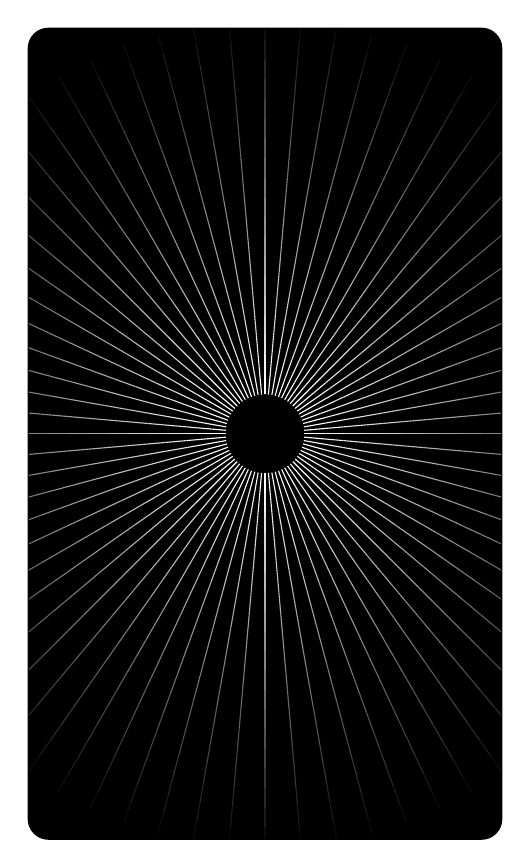
\begin{tikzpicture}
  \draw[rounded corners=2.5mm, thick] (0,0) rectangle (\cardwidth, \cardheight);
  \clip[rounded corners=2.5mm] (0,0) rectangle (\cardwidth, \cardheight);
  \fill[black] (0,0) rectangle (\cardwidth, \cardheight);
  \foreach \a in {0,5,...,355} {
    \foreach \s in {0,1,...,19} {
      \pgfmathsetmacro{\op}{1 - \s/19}%
      \pgfmathsetmacro{\startrad}{5 + \s*2.5}%
      \draw[white, thin, opacity=\op]
        (0.5\cardwidth, 0.5\cardheight) ++(\a:\startrad mm) -- ++(\a:2.5mm);
    }
  }
\end{tikzpicture}%
}

\newpage
\noindent
\cardback\hfill
\cardback\hfill
\cardback

\vspace{4mm}
\noindent
\cardback\hfill
\cardback\hfill
\cardback

\end{document}
